\documentclass[a4paper]{book}
\usepackage{a4wide}
\usepackage{makeidx}
\usepackage{graphicx}
\usepackage{multicol}
\usepackage{float}
\usepackage{listings}
\usepackage{color}
\usepackage{textcomp}
\usepackage{alltt}
\usepackage{times}
\usepackage{ifpdf}
\ifpdf
\usepackage[pdftex,
            pagebackref=true,
            colorlinks=true,
            linkcolor=blue,
            unicode
           ]{hyperref}
\else
\usepackage[ps2pdf,
            pagebackref=true,
            colorlinks=true,
            linkcolor=blue,
            unicode
           ]{hyperref}
\usepackage{pspicture}
\fi
\usepackage[utf8]{inputenc}
\usepackage{doxygen}
\lstset{language=C++,inputencoding=utf8,basicstyle=\footnotesize,breaklines=true,breakatwhitespace=true,tabsize=8,numbers=left }
\makeindex
\setcounter{tocdepth}{3}
\renewcommand{\footrulewidth}{0.4pt}
\begin{document}
\hypersetup{pageanchor=false}
\begin{titlepage}
\vspace*{7cm}
\begin{center}
{\Large BGL Interface }\\
\vspace*{1cm}
{\large Generated by Doxygen 1.6.1}\\
\vspace*{0.5cm}
{\small Mon Oct 24 17:21:34 2016}\\
\end{center}
\end{titlepage}
\clearemptydoublepage
\pagenumbering{roman}
\tableofcontents
\clearemptydoublepage
\pagenumbering{arabic}
\hypersetup{pageanchor=true}
\chapter{Todo List}
\label{todo}
\hypertarget{todo}{}
\label{todo__todo000001}
\hypertarget{todo__todo000001}{}
 
\begin{DoxyDescription}
\item[Class \hyperlink{structGeometry_1_1Intersection}{Geometry::Intersection} ]It can be bettered by adding another attribute that indicates, in the case of two edges end which coincides the relative position on the edge. It requires a simple modification of the function segmentIntersect 
\end{DoxyDescription}
\chapter{Class Index}
\section{Class Hierarchy}
This inheritance list is sorted roughly, but not completely, alphabetically:\begin{DoxyCompactList}
\item \contentsline{section}{circular\_\-edge\_\-geometry}{\pageref{classcircular__edge__geometry}}{}
\item \contentsline{section}{data\_\-structure$<$ Edge\_\-data\_\-structure, Vertex\_\-data\_\-structure $>$}{\pageref{structdata__structure}}{}
\item \contentsline{section}{edge\_\-data\_\-structure$<$ dim $>$}{\pageref{structedge__data__structure}}{}
\item \contentsline{section}{BGLgeom::edge\_\-geometry$<$ dim $>$}{\pageref{classBGLgeom_1_1edge__geometry}}{}
\begin{DoxyCompactList}
\item \contentsline{section}{BGLgeom::generic\_\-edge\_\-geometry$<$ dim $>$}{\pageref{classBGLgeom_1_1generic__edge__geometry}}{}
\end{DoxyCompactList}
\item \contentsline{section}{edge\_\-parametrization}{\pageref{classedge__parametrization}}{}
\item \contentsline{section}{edge\_\-prop\_\-max\_\-flow\_\-t}{\pageref{structedge__prop__max__flow__t}}{}
\item \contentsline{section}{Forma\_\-edge\_\-property\_\-t}{\pageref{structForma__edge__property__t}}{}
\item \contentsline{section}{Forma\_\-vertex\_\-property\_\-t}{\pageref{structForma__vertex__property__t}}{}
\item \contentsline{section}{Geometry::Intersection}{\pageref{structGeometry_1_1Intersection}}{}
\item \contentsline{section}{intersector\_\-base\_\-class$<$ Graph $>$}{\pageref{classintersector__base__class}}{}
\begin{DoxyCompactList}
\item \contentsline{section}{final$<$ Graph $>$}{\pageref{classfinal}}{}
\end{DoxyCompactList}
\item \contentsline{section}{Geometry::Linear\_\-edge}{\pageref{classGeometry_1_1Linear__edge}}{}
\item \contentsline{section}{my\_\-edge}{\pageref{structmy__edge}}{}
\item \contentsline{section}{new\_\-reader\_\-class$<$ Source\_\-data\_\-structure, Target\_\-data\_\-structure, Edge\_\-data\_\-structure, Topological\_\-data\_\-structure $>$}{\pageref{classnew__reader__class}}{}
\item \contentsline{section}{new\_\-reader\_\-class$<$ Zunino\_\-source\_\-data, Zunino\_\-target\_\-data, Zunino\_\-edge\_\-data, Zunino\_\-topological\_\-data $>$}{\pageref{classnew__reader__class}}{}
\begin{DoxyCompactList}
\item \contentsline{section}{Zunino\_\-reader$<$ Zunino\_\-source\_\-data, Zunino\_\-target\_\-data, Zunino\_\-edge\_\-data, Zunino\_\-topological\_\-data $>$}{\pageref{classZunino__reader}}{}
\end{DoxyCompactList}
\item \contentsline{section}{no\_\-topological\_\-data}{\pageref{structno__topological__data}}{}
\item \contentsline{section}{our\_\-disjoint\_\-sets$<$ Graph $>$}{\pageref{classour__disjoint__sets}}{}
\item \contentsline{section}{BGLgeom::point$<$ dim, Storage\_\-t $>$}{\pageref{classBGLgeom_1_1point}}{}
\item \contentsline{section}{reader\_\-base\_\-class$<$ Graph $>$}{\pageref{classreader__base__class}}{}
\begin{DoxyCompactList}
\item \contentsline{section}{final$<$ Graph $>$}{\pageref{classfinal}}{}
\item \contentsline{section}{final$<$ Graph $>$}{\pageref{classfinal}}{}
\end{DoxyCompactList}
\item \contentsline{section}{vertex\_\-data\_\-structure$<$ dim $>$}{\pageref{structvertex__data__structure}}{}
\item \contentsline{section}{Zunino\_\-edge\_\-data}{\pageref{structZunino__edge__data}}{}
\item \contentsline{section}{Zunino\_\-edge\_\-property\_\-t}{\pageref{structZunino__edge__property__t}}{}
\item \contentsline{section}{Zunino\_\-source\_\-data}{\pageref{structZunino__source__data}}{}
\item \contentsline{section}{Zunino\_\-target\_\-data}{\pageref{structZunino__target__data}}{}
\item \contentsline{section}{Zunino\_\-topological\_\-data}{\pageref{structZunino__topological__data}}{}
\end{DoxyCompactList}

\chapter{Class Index}
\section{Class List}
Here are the classes, structs, unions and interfaces with brief descriptions:\begin{DoxyCompactList}
\item\contentsline{section}{\hyperlink{classcircular__edge__geometry}{circular\_\-edge\_\-geometry} }{\pageref{classcircular__edge__geometry}}{}
\item\contentsline{section}{\hyperlink{structdata__structure}{data\_\-structure$<$ Edge\_\-data\_\-structure, Vertex\_\-data\_\-structure $>$} (An abstract class to handle the user definition data structure  The users has to specify, in the derived class, all variables he need in order to store information read from the input file. Then, through the definition of Edge\_\-data\_\-structure and Vertex\_\-data\_\-structure, he can get separately all the information to put on edges and vertices )}{\pageref{structdata__structure}}{}
\item\contentsline{section}{\hyperlink{structedge__data__structure}{edge\_\-data\_\-structure$<$ dim $>$} }{\pageref{structedge__data__structure}}{}
\item\contentsline{section}{\hyperlink{classBGLgeom_1_1edge__geometry}{BGLgeom::edge\_\-geometry$<$ dim $>$} }{\pageref{classBGLgeom_1_1edge__geometry}}{}
\item\contentsline{section}{\hyperlink{classedge__parametrization}{edge\_\-parametrization} (This class holds the parametrization of the edge )}{\pageref{classedge__parametrization}}{}
\item\contentsline{section}{\hyperlink{structedge__prop__max__flow__t}{edge\_\-prop\_\-max\_\-flow\_\-t} }{\pageref{structedge__prop__max__flow__t}}{}
\item\contentsline{section}{\hyperlink{classfinal}{final$<$ Graph $>$} }{\pageref{classfinal}}{}
\item\contentsline{section}{\hyperlink{structForma__edge__property__t}{Forma\_\-edge\_\-property\_\-t} }{\pageref{structForma__edge__property__t}}{}
\item\contentsline{section}{\hyperlink{structForma__vertex__property__t}{Forma\_\-vertex\_\-property\_\-t} (This struct contains the vertex property for Formaggia's example )}{\pageref{structForma__vertex__property__t}}{}
\item\contentsline{section}{\hyperlink{classBGLgeom_1_1generic__edge__geometry}{BGLgeom::generic\_\-edge\_\-geometry$<$ dim $>$} }{\pageref{classBGLgeom_1_1generic__edge__geometry}}{}
\item\contentsline{section}{\hyperlink{structGeometry_1_1Intersection}{Geometry::Intersection} (A simple struct that contains the result of the intersection test )}{\pageref{structGeometry_1_1Intersection}}{}
\item\contentsline{section}{\hyperlink{classintersector__base__class}{intersector\_\-base\_\-class$<$ Graph $>$} }{\pageref{classintersector__base__class}}{}
\item\contentsline{section}{\hyperlink{classGeometry_1_1Linear__edge}{Geometry::Linear\_\-edge} (A simple class that hanlde a linear edge  This class is thought to manage the description of the geometry of a linear edge, in order to compute intersections )}{\pageref{classGeometry_1_1Linear__edge}}{}
\item\contentsline{section}{\hyperlink{structmy__edge}{my\_\-edge} }{\pageref{structmy__edge}}{}
\item\contentsline{section}{\hyperlink{classnew__reader__class}{new\_\-reader\_\-class$<$ Source\_\-data\_\-structure, Target\_\-data\_\-structure, Edge\_\-data\_\-structure, Topological\_\-data\_\-structure $>$} (Abstract class that implements the functionality to read a file and get data from it  The users has to specify, in the derived class, all variables he need in order to store information read from the input file. Then, through the definition of Edge\_\-data\_\-structure and Vertex\_\-data\_\-structure, he can get separately all the information to put on edges and vertices )}{\pageref{classnew__reader__class}}{}
\item\contentsline{section}{\hyperlink{structno__topological__data}{no\_\-topological\_\-data} (An empty struct to handle the case the user do not need to store topological data  Inside this the user may put data as vertex and edge descriptor for the connettivity of the graph )}{\pageref{structno__topological__data}}{}
\item\contentsline{section}{\hyperlink{classour__disjoint__sets}{our\_\-disjoint\_\-sets$<$ Graph $>$} (Template class to handle disjoint sets  The template parameters are:\par
 Label\_\-map\_\-t: the type of a std::map which key is a vertex descriptor and the value is an unsigned int which has the meaning of the current label of the component to which that vertex belongs to.\par
 Components\_\-map\_\-t: the type of a std::map which key is an unsigned int used as label for the group and the value is a std::set containing all the vertex descriptor of the vertices that have that label, i.e that belong to the same component )}{\pageref{classour__disjoint__sets}}{}
\item\contentsline{section}{\hyperlink{classBGLgeom_1_1point}{BGLgeom::point$<$ dim, Storage\_\-t $>$} (Class template for storing the vertex coordinates in n-\/dimentional space )}{\pageref{classBGLgeom_1_1point}}{}
\item\contentsline{section}{\hyperlink{classreader__base__class}{reader\_\-base\_\-class$<$ Graph $>$} }{\pageref{classreader__base__class}}{}
\item\contentsline{section}{\hyperlink{structvertex__data__structure}{vertex\_\-data\_\-structure$<$ dim $>$} }{\pageref{structvertex__data__structure}}{}
\item\contentsline{section}{\hyperlink{structZunino__edge__data}{Zunino\_\-edge\_\-data} }{\pageref{structZunino__edge__data}}{}
\item\contentsline{section}{\hyperlink{structZunino__edge__property__t}{Zunino\_\-edge\_\-property\_\-t} }{\pageref{structZunino__edge__property__t}}{}
\item\contentsline{section}{\hyperlink{classZunino__reader}{Zunino\_\-reader$<$ Zunino\_\-source\_\-data, Zunino\_\-target\_\-data, Zunino\_\-edge\_\-data, Zunino\_\-topological\_\-data $>$} }{\pageref{classZunino__reader}}{}
\item\contentsline{section}{\hyperlink{structZunino__source__data}{Zunino\_\-source\_\-data} }{\pageref{structZunino__source__data}}{}
\item\contentsline{section}{\hyperlink{structZunino__target__data}{Zunino\_\-target\_\-data} }{\pageref{structZunino__target__data}}{}
\item\contentsline{section}{\hyperlink{structZunino__topological__data}{Zunino\_\-topological\_\-data} }{\pageref{structZunino__topological__data}}{}
\end{DoxyCompactList}

\chapter{File Index}
\section{File List}
Here is a list of all documented files with brief descriptions:\begin{DoxyCompactList}
\item\contentsline{section}{include/{\bfseries circular\_\-edge\_\-geometry.hpp} }{\pageref{circular__edge__geometry_8hpp}}{}
\item\contentsline{section}{include/\hyperlink{compute__euclidean__distance_8hpp}{compute\_\-euclidean\_\-distance.hpp} (Computes the euclidean distance between two given vertices )}{\pageref{compute__euclidean__distance_8hpp}}{}
\item\contentsline{section}{include/{\bfseries compute\_\-euclidean\_\-distance\_\-imp.hpp} }{\pageref{compute__euclidean__distance__imp_8hpp}}{}
\item\contentsline{section}{include/\hyperlink{data__structure_8hpp}{data\_\-structure.hpp} (Declaration of generic data structure to represent vertex and edge properties )}{\pageref{data__structure_8hpp}}{}
\item\contentsline{section}{include/\hyperlink{dijkstra_8hpp}{dijkstra.hpp} (Solves the single-\/source shortest-\/paths problem on a weighted, directed graph with non-\/negative edge weights.  This function takes in input the graph, the source vertex and two vectors, one for the distance map and the other for the predecessor map, which will be filled with the results of the algorithm )}{\pageref{dijkstra_8hpp}}{}
\item\contentsline{section}{include/\hyperlink{dijkstra__imp_8hpp}{dijkstra\_\-imp.hpp} (Solves the single-\/source shortest-\/paths problem on a weighted, directed graph with non-\/negative edge weights.  )}{\pageref{dijkstra__imp_8hpp}}{}
\item\contentsline{section}{include/\hyperlink{disjoint__components_8hpp}{disjoint\_\-components.hpp} (Identifies if there are fully disconnected subgraphs..  )}{\pageref{disjoint__components_8hpp}}{}
\item\contentsline{section}{include/\hyperlink{disjoint__components__imp_8hpp}{disjoint\_\-components\_\-imp.hpp} (Identifies if there are fully disconnected subgraphs )}{\pageref{disjoint__components__imp_8hpp}}{}
\item\contentsline{section}{include/\hyperlink{edge__geometry_8hpp}{edge\_\-geometry.hpp} (Virtual base class for the geometry of an edge  )}{\pageref{edge__geometry_8hpp}}{}
\item\contentsline{section}{include/{\bfseries edge\_\-property\_\-max\_\-flow.hpp} }{\pageref{edge__property__max__flow_8hpp}}{}
\item\contentsline{section}{include/\hyperlink{Forma__edge__property_8hpp}{Forma\_\-edge\_\-property.hpp} (This contains the struct for edge properties that has to be used for Formaggia's example  )}{\pageref{Forma__edge__property_8hpp}}{}
\item\contentsline{section}{include/\hyperlink{Forma__vertex__property_8hpp}{Forma\_\-vertex\_\-property.hpp} (This contains the struct for vertex properties that has to be used for Formaggia's example  )}{\pageref{Forma__vertex__property_8hpp}}{}
\item\contentsline{section}{include/\hyperlink{generic__edge__geometry_8hpp}{generic\_\-edge\_\-geometry.hpp} (Class for circular geometry of an edge  )}{\pageref{generic__edge__geometry_8hpp}}{}
\item\contentsline{section}{include/\hyperlink{generic__point_8hpp}{generic\_\-point.hpp} (Templete class to handle points in 2D or 3D (or even greater) )}{\pageref{generic__point_8hpp}}{}
\item\contentsline{section}{include/\hyperlink{graph__builder_8hpp}{graph\_\-builder.hpp} (Utilities to build a graph )}{\pageref{graph__builder_8hpp}}{}
\item\contentsline{section}{include/\hyperlink{intersector__base__class_8hpp}{intersector\_\-base\_\-class.hpp} (Abstract class to handle intersections of edges in a graph with geometrical properties  It contains also some utilities needed to compute the intersection between two (linear) edges )}{\pageref{intersector__base__class_8hpp}}{}
\item\contentsline{section}{include/\hyperlink{io__graph_8hpp}{io\_\-graph.hpp} (Declaration of functions related to input and output of the graph )}{\pageref{io__graph_8hpp}}{}
\item\contentsline{section}{include/\hyperlink{io__graph__imp_8hpp}{io\_\-graph\_\-imp.hpp} (Definition of functions related to input and output of the graph )}{\pageref{io__graph__imp_8hpp}}{}
\item\contentsline{section}{include/\hyperlink{maximum__flow_8hpp}{maximum\_\-flow.hpp} (Header file for managing maximum\_\-flow algorithm from BGL )}{\pageref{maximum__flow_8hpp}}{}
\item\contentsline{section}{include/\hyperlink{maximum__flow__imp_8hpp}{maximum\_\-flow\_\-imp.hpp} (Implementations of the functions defined in \hyperlink{maximum__flow_8hpp}{maximum\_\-flow.hpp} )}{\pageref{maximum__flow__imp_8hpp}}{}
\item\contentsline{section}{include/\hyperlink{new__reader__class_8hpp}{new\_\-reader\_\-class.hpp} (Base abstract class to read input file )}{\pageref{new__reader__class_8hpp}}{}
\item\contentsline{section}{include/\hyperlink{new__reader__Zunino_8hpp}{new\_\-reader\_\-Zunino.hpp} (Class for reading from Zunino files )}{\pageref{new__reader__Zunino_8hpp}}{}
\item\contentsline{section}{include/\hyperlink{our__disjoint__sets_8hpp}{our\_\-disjoint\_\-sets.hpp} (Class to handle disjoint sets  )}{\pageref{our__disjoint__sets_8hpp}}{}
\item\contentsline{section}{include/\hyperlink{reader__base__class_8hpp}{reader\_\-base\_\-class.hpp} (Base abstract class to read input file and creating the graph )}{\pageref{reader__base__class_8hpp}}{}
\item\contentsline{section}{include/\hyperlink{reader__Formaggia__class_8hpp}{reader\_\-Formaggia\_\-class.hpp} (Implementation of the \hyperlink{classreader__base__class}{reader\_\-base\_\-class} for the Formaggia file format )}{\pageref{reader__Formaggia__class_8hpp}}{}
\item\contentsline{section}{include/\hyperlink{reader__Zunino__class_8hpp}{reader\_\-Zunino\_\-class.hpp} (Implementation of the reader for Zunino file format )}{\pageref{reader__Zunino__class_8hpp}}{}
\item\contentsline{section}{include/\hyperlink{topological__distance_8hpp}{topological\_\-distance.hpp} (Computes topological distance.  )}{\pageref{topological__distance_8hpp}}{}
\item\contentsline{section}{include/\hyperlink{topological__distance__imp_8hpp}{topological\_\-distance\_\-imp.hpp} (Computes topological distance.  )}{\pageref{topological__distance__imp_8hpp}}{}
\item\contentsline{section}{include/\hyperlink{Zunino__edge__property_8hpp}{Zunino\_\-edge\_\-property.hpp} (Contains the struct for edge properties in Zunino's problem )}{\pageref{Zunino__edge__property_8hpp}}{}
\item\contentsline{section}{src/\hyperlink{main__Formaggia_8cpp}{main\_\-Formaggia.cpp} (Source code for Formaggia's example  )}{\pageref{main__Formaggia_8cpp}}{}
\item\contentsline{section}{src/\hyperlink{main__Zunino_8cpp}{main\_\-Zunino.cpp} (Source code for Zunino example.  )}{\pageref{main__Zunino_8cpp}}{}
\end{DoxyCompactList}

\chapter{Class Documentation}
\hypertarget{classcircular__edge__geometry}{
\section{circular\_\-edge\_\-geometry Class Reference}
\label{classcircular__edge__geometry}\index{circular\_\-edge\_\-geometry@{circular\_\-edge\_\-geometry}}
}
\subsection*{Public Member Functions}
\begin{DoxyCompactItemize}
\item 
\hypertarget{classcircular__edge__geometry_a0efaab032d5334baa83aa80ebc53fc9b}{
{\bfseries circular\_\-edge\_\-geometry} (point center\_\-, double start\_\-angle\_\-, double end\_\-angle\_\-)}
\label{classcircular__edge__geometry_a0efaab032d5334baa83aa80ebc53fc9b}

\item 
\hypertarget{classcircular__edge__geometry_abe44d1d8bb11bf92fc105757f478ff48}{
point {\bfseries value} (double parameter)}
\label{classcircular__edge__geometry_abe44d1d8bb11bf92fc105757f478ff48}

\end{DoxyCompactItemize}


The documentation for this class was generated from the following file:\begin{DoxyCompactItemize}
\item 
include/circular\_\-edge\_\-geometry.hpp\end{DoxyCompactItemize}

\hypertarget{structdata__structure}{
\section{data\_\-structure$<$ Edge\_\-data\_\-structure, Vertex\_\-data\_\-structure $>$ Class Template Reference}
\label{structdata__structure}\index{data\_\-structure@{data\_\-structure}}
}


An abstract class to handle the user definition data structure  The users has to specify, in the derived class, all variables he need in order to store information read from the input file. Then, through the definition of Edge\_\-data\_\-structure and Vertex\_\-data\_\-structure, he can get separately all the information to put on edges and vertices.  


{\ttfamily \#include $<$data\_\-structure.hpp$>$}\subsection*{Public Member Functions}
\begin{DoxyCompactItemize}
\item 
\hypertarget{structdata__structure_a08a8f29045d2c69e957a4e3120d7af10}{
virtual Edge\_\-data\_\-structure \hyperlink{structdata__structure_a08a8f29045d2c69e957a4e3120d7af10}{get\_\-edge\_\-data} ()=0}
\label{structdata__structure_a08a8f29045d2c69e957a4e3120d7af10}

\begin{DoxyCompactList}\small\item\em A method to get the right data to append to an edge. \item\end{DoxyCompactList}\item 
\hypertarget{structdata__structure_a01fbb29b47afaae30a6d2652ae82f90e}{
virtual Vertex\_\-data\_\-structure \hyperlink{structdata__structure_a01fbb29b47afaae30a6d2652ae82f90e}{get\_\-vertex\_\-data} ()=0}
\label{structdata__structure_a01fbb29b47afaae30a6d2652ae82f90e}

\begin{DoxyCompactList}\small\item\em A method to get the right data to append to a vertex. \item\end{DoxyCompactList}\item 
\hypertarget{structdata__structure_a9746c1f03a1a9c73571c59653a14650d}{
virtual void \hyperlink{structdata__structure_a9746c1f03a1a9c73571c59653a14650d}{get\_\-data\_\-from\_\-line} (std::ifstream \&, \hyperlink{structdata__structure}{data\_\-structure} \&)=0}
\label{structdata__structure_a9746c1f03a1a9c73571c59653a14650d}

\begin{DoxyCompactList}\small\item\em The way the data from the input file are read  User has to specify how to read data from input file. \item\end{DoxyCompactList}\end{DoxyCompactItemize}


\subsection{Detailed Description}
\subsubsection*{template$<$typename Edge\_\-data\_\-structure, typename Vertex\_\-data\_\-structure$>$ class data\_\-structure$<$ Edge\_\-data\_\-structure, Vertex\_\-data\_\-structure $>$}

An abstract class to handle the user definition data structure  The users has to specify, in the derived class, all variables he need in order to store information read from the input file. Then, through the definition of Edge\_\-data\_\-structure and Vertex\_\-data\_\-structure, he can get separately all the information to put on edges and vertices. 
\begin{DoxyParams}{Parameters}
\item[{\em Edge\_\-data\_\-structure}]A struct where the user has to define type and name of the variables he needs to append to vertices as vertex bundled property \item[{\em Vertex\_\-data\_\-structure}]A struct where the user has to define type and name of the variables he needs to append to edge as edge bundled property \end{DoxyParams}
\begin{DoxyPrecond}{Precondition}
It may be useful to declare a friend operator$>$$>$ to help the reader read the data 
\end{DoxyPrecond}


The documentation for this class was generated from the following file:\begin{DoxyCompactItemize}
\item 
include/\hyperlink{data__structure_8hpp}{data\_\-structure.hpp}\end{DoxyCompactItemize}

\hypertarget{structedge__data__structure}{
\section{edge\_\-data\_\-structure$<$ dim $>$ Struct Template Reference}
\label{structedge__data__structure}\index{edge\_\-data\_\-structure@{edge\_\-data\_\-structure}}
}
\subsection*{Public Attributes}
\begin{DoxyCompactItemize}
\item 
\hypertarget{structedge__data__structure_aec41c0f9780370b8650c7ee0f543f7ab}{
unsigned int {\bfseries edge\_\-id} = 0}
\label{structedge__data__structure_aec41c0f9780370b8650c7ee0f543f7ab}

\item 
\hypertarget{structedge__data__structure_a2c23e71c2fd29d1a400b916992668774}{
std::string {\bfseries label} = \char`\"{}\char`\"{}}
\label{structedge__data__structure_a2c23e71c2fd29d1a400b916992668774}

\item 
\hypertarget{structedge__data__structure_a6842d811177dd1603b5436a8e38e1457}{
double {\bfseries lenght} = 0}
\label{structedge__data__structure_a6842d811177dd1603b5436a8e38e1457}

\item 
\hypertarget{structedge__data__structure_af69d7d380e0e2b79f15c2b5af07e8afe}{
double {\bfseries capacity} = 0}
\label{structedge__data__structure_af69d7d380e0e2b79f15c2b5af07e8afe}

\item 
\hypertarget{structedge__data__structure_a2ff81a66e3636a6b1b323dfb04ce36e2}{
double {\bfseries diameter} = 0}
\label{structedge__data__structure_a2ff81a66e3636a6b1b323dfb04ce36e2}

\item 
\hypertarget{structedge__data__structure_a2dc5eb72ac308fddb9f4bd6510ff387c}{
double {\bfseries weight} = 0}
\label{structedge__data__structure_a2dc5eb72ac308fddb9f4bd6510ff387c}

\item 
\hypertarget{structedge__data__structure_a1d0b2d0bd57d916e472a7f3ec0d4d94e}{
generic\_\-edge\_\-geometry$<$ dim $>$ {\bfseries edge\_\-geo}}
\label{structedge__data__structure_a1d0b2d0bd57d916e472a7f3ec0d4d94e}

\end{DoxyCompactItemize}
\subsubsection*{template$<$unsigned int dim$>$ struct edge\_\-data\_\-structure$<$ dim $>$}



The documentation for this struct was generated from the following file:\begin{DoxyCompactItemize}
\item 
include/\hyperlink{data__structure_8hpp}{data\_\-structure.hpp}\end{DoxyCompactItemize}

\hypertarget{classBGLgeom_1_1edge__geometry}{
\section{BGLgeom::edge\_\-geometry$<$ dim $>$ Class Template Reference}
\label{classBGLgeom_1_1edge__geometry}\index{BGLgeom::edge\_\-geometry@{BGLgeom::edge\_\-geometry}}
}
Inheritance diagram for BGLgeom::edge\_\-geometry$<$ dim $>$::\begin{figure}[H]
\begin{center}
\leavevmode
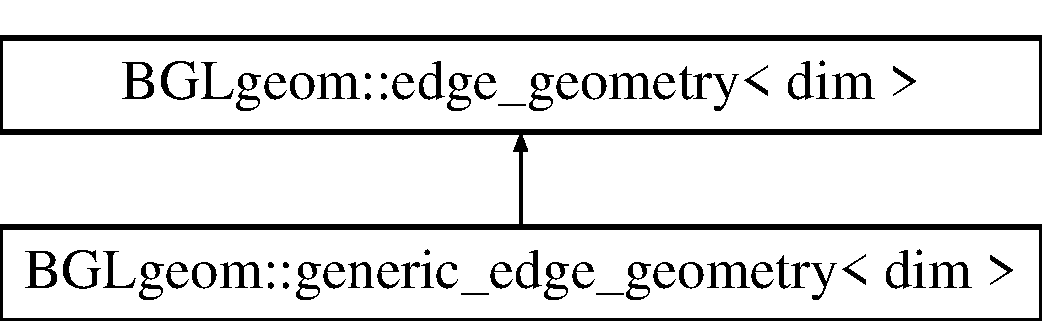
\includegraphics[height=2cm]{classBGLgeom_1_1edge__geometry}
\end{center}
\end{figure}
\subsection*{Public Member Functions}
\begin{DoxyCompactItemize}
\item 
\hypertarget{classBGLgeom_1_1edge__geometry_ae4e0868c01e2e490eea053e6942b0aef}{
virtual \hyperlink{classBGLgeom_1_1point}{BGLgeom::point}$<$ dim $>$ {\bfseries value} (const double parameter)=0}
\label{classBGLgeom_1_1edge__geometry_ae4e0868c01e2e490eea053e6942b0aef}

\item 
\hypertarget{classBGLgeom_1_1edge__geometry_a41d857a2978d96127fc1797232183844}{
virtual std::vector$<$ double $>$ {\bfseries first\_\-derivatives} (const double x)=0}
\label{classBGLgeom_1_1edge__geometry_a41d857a2978d96127fc1797232183844}

\item 
\hypertarget{classBGLgeom_1_1edge__geometry_a29e57f380b8a1fe071a5a51b42873408}{
virtual std::vector$<$ double $>$ {\bfseries second\_\-derivatives} (const double x)=0}
\label{classBGLgeom_1_1edge__geometry_a29e57f380b8a1fe071a5a51b42873408}

\end{DoxyCompactItemize}
\subsubsection*{template$<$unsigned int dim$>$ class BGLgeom::edge\_\-geometry$<$ dim $>$}



The documentation for this class was generated from the following file:\begin{DoxyCompactItemize}
\item 
include/\hyperlink{edge__geometry_8hpp}{edge\_\-geometry.hpp}\end{DoxyCompactItemize}

\hypertarget{classedge__parametrization}{
\section{edge\_\-parametrization Class Reference}
\label{classedge__parametrization}\index{edge\_\-parametrization@{edge\_\-parametrization}}
}


This class holds the parametrization of the edge.  


{\ttfamily \#include $<$Forma\_\-edge\_\-property.hpp$>$}

\subsection{Detailed Description}
This class holds the parametrization of the edge. 

The documentation for this class was generated from the following file:\begin{DoxyCompactItemize}
\item 
include/\hyperlink{Forma__edge__property_8hpp}{Forma\_\-edge\_\-property.hpp}\end{DoxyCompactItemize}

\hypertarget{structedge__prop__max__flow__t}{
\section{edge\_\-prop\_\-max\_\-flow\_\-t Struct Reference}
\label{structedge__prop__max__flow__t}\index{edge\_\-prop\_\-max\_\-flow\_\-t@{edge\_\-prop\_\-max\_\-flow\_\-t}}
}
\subsection*{Public Attributes}
\begin{DoxyCompactItemize}
\item 
\hypertarget{structedge__prop__max__flow__t_ab9327d96f83b603c8641661a37383559}{
double {\bfseries capacity}}
\label{structedge__prop__max__flow__t_ab9327d96f83b603c8641661a37383559}

\item 
\hypertarget{structedge__prop__max__flow__t_afbc4c3225a82ae95bd1eb724366b62e0}{
double {\bfseries residual\_\-capacity}}
\label{structedge__prop__max__flow__t_afbc4c3225a82ae95bd1eb724366b62e0}

\item 
\hypertarget{structedge__prop__max__flow__t_a72d9d421e60fe1fc3cfe59a35ef48697}{
bool {\bfseries original\_\-edge}}
\label{structedge__prop__max__flow__t_a72d9d421e60fe1fc3cfe59a35ef48697}

\end{DoxyCompactItemize}


The documentation for this struct was generated from the following file:\begin{DoxyCompactItemize}
\item 
include/edge\_\-property\_\-max\_\-flow.hpp\end{DoxyCompactItemize}

\hypertarget{classfinal}{
\section{final$<$ Graph $>$ Class Template Reference}
\label{classfinal}\index{final@{final}}
}
Inheritance diagram for final$<$ Graph $>$::\begin{figure}[H]
\begin{center}
\leavevmode
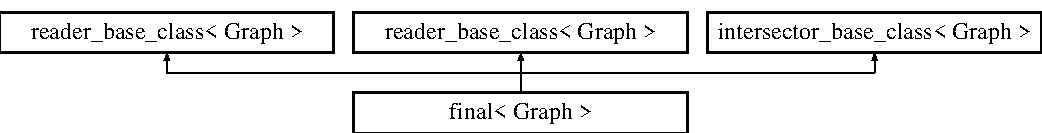
\includegraphics[height=1.78628cm]{classfinal}
\end{center}
\end{figure}
\subsection*{Public Types}
\begin{DoxyCompactItemize}
\item 
\hypertarget{classfinal_a71a55ce0e3a3e740da4d8958b2ce3b2a}{
typedef \hyperlink{classreader__base__class}{reader\_\-base\_\-class}$<$ Graph $>$::Vertex\_\-desc {\bfseries Vertex\_\-desc}}
\label{classfinal_a71a55ce0e3a3e740da4d8958b2ce3b2a}

\item 
\hypertarget{classfinal_a7a618f6a143db77a7ea54d7cd11ae607}{
typedef \hyperlink{classreader__base__class}{reader\_\-base\_\-class}$<$ Graph $>$::Edge\_\-desc {\bfseries Edge\_\-desc}}
\label{classfinal_a7a618f6a143db77a7ea54d7cd11ae607}

\item 
\hypertarget{classfinal_a22c478f61e09f8d21e659cda4a5ef674}{
typedef \hyperlink{classintersector__base__class}{intersector\_\-base\_\-class}$<$ Graph $>$::Edge\_\-iter {\bfseries Edge\_\-iter}}
\label{classfinal_a22c478f61e09f8d21e659cda4a5ef674}

\item 
\hypertarget{classfinal_a828f09fa919dbb68e143a6eb94e93696}{
typedef \hyperlink{classintersector__base__class}{intersector\_\-base\_\-class}$<$ Graph $>$::Intersections\_\-type {\bfseries Intersections\_\-type}}
\label{classfinal_a828f09fa919dbb68e143a6eb94e93696}

\item 
\hypertarget{classfinal_a71a55ce0e3a3e740da4d8958b2ce3b2a}{
typedef \hyperlink{classreader__base__class}{reader\_\-base\_\-class}$<$ Graph $>$::Vertex\_\-desc {\bfseries Vertex\_\-desc}}
\label{classfinal_a71a55ce0e3a3e740da4d8958b2ce3b2a}

\item 
\hypertarget{classfinal_a7a618f6a143db77a7ea54d7cd11ae607}{
typedef \hyperlink{classreader__base__class}{reader\_\-base\_\-class}$<$ Graph $>$::Edge\_\-desc {\bfseries Edge\_\-desc}}
\label{classfinal_a7a618f6a143db77a7ea54d7cd11ae607}

\end{DoxyCompactItemize}
\subsection*{Public Member Functions}
\begin{DoxyCompactItemize}
\item 
\hypertarget{classfinal_ac405f6106b4f8e90cb06dd52284983c2}{
\hyperlink{classfinal_ac405f6106b4f8e90cb06dd52284983c2}{reader\_\-Formaggia} (Graph \&\_\-G)}
\label{classfinal_ac405f6106b4f8e90cb06dd52284983c2}

\begin{DoxyCompactList}\small\item\em Default constructor (we need however to initialize the reference to the graph). \item\end{DoxyCompactList}\item 
\hypertarget{classfinal_a712036b0fd3396380d5c393453929f29}{
\hyperlink{classfinal_a712036b0fd3396380d5c393453929f29}{reader\_\-Formaggia} (Graph \&\_\-G, std::string \_\-file\_\-name, unsigned int \_\-num\_\-dummy\_\-lines)}
\label{classfinal_a712036b0fd3396380d5c393453929f29}

\begin{DoxyCompactList}\small\item\em Constructor. \item\end{DoxyCompactList}\item 
\hypertarget{classfinal_a5be0850fa08372356ff146355b887693}{
\hyperlink{classfinal_a5be0850fa08372356ff146355b887693}{reader\_\-Formaggia} (reader\_\-Formaggia const \&)}
\label{classfinal_a5be0850fa08372356ff146355b887693}

\begin{DoxyCompactList}\small\item\em Default copy constructor. \item\end{DoxyCompactList}\item 
\hypertarget{classfinal_a02e28eddd4f99661a55bd9f52641db44}{
reader\_\-Formaggia \& \hyperlink{classfinal_a02e28eddd4f99661a55bd9f52641db44}{operator=} (reader\_\-Formaggia const \&)}
\label{classfinal_a02e28eddd4f99661a55bd9f52641db44}

\begin{DoxyCompactList}\small\item\em Default assignment operator. \item\end{DoxyCompactList}\item 
\hypertarget{classfinal_a459de677ac9395a35062c28c523bf4a3}{
virtual \hyperlink{classfinal_a459de677ac9395a35062c28c523bf4a3}{$\sim$reader\_\-Formaggia} ()}
\label{classfinal_a459de677ac9395a35062c28c523bf4a3}

\begin{DoxyCompactList}\small\item\em Destructor. \item\end{DoxyCompactList}\item 
\hypertarget{classfinal_a8f6841bfff9cfdc1127b8290a1ef1085}{
void \hyperlink{classfinal_a8f6841bfff9cfdc1127b8290a1ef1085}{set\_\-e\_\-to\_\-be\_\-removed} (Edge\_\-desc const \&\_\-e\_\-to\_\-be\_\-removed)}
\label{classfinal_a8f6841bfff9cfdc1127b8290a1ef1085}

\begin{DoxyCompactList}\small\item\em It allows to set e\_\-to\_\-be\_\-removed. \item\end{DoxyCompactList}\item 
\hypertarget{classfinal_aa61075494cf1aea32b10f216fb9093fc}{
void \hyperlink{classfinal_aa61075494cf1aea32b10f216fb9093fc}{set\_\-split\_\-edge} (Edge\_\-desc const \&\_\-split\_\-edge)}
\label{classfinal_aa61075494cf1aea32b10f216fb9093fc}

\begin{DoxyCompactList}\small\item\em It allows to set split\_\-edge. \item\end{DoxyCompactList}\item 
\hypertarget{classfinal_a0312312e30a4b59f9e1c861539f266ec}{
void \hyperlink{classfinal_a0312312e30a4b59f9e1c861539f266ec}{set\_\-intersection\_\-new} (Vertex\_\-desc const \&\_\-intersection\_\-new)}
\label{classfinal_a0312312e30a4b59f9e1c861539f266ec}

\begin{DoxyCompactList}\small\item\em It allows to set intersection\_\-new. \item\end{DoxyCompactList}\item 
\hypertarget{classfinal_a0085254883aa39b135d51794d75d3ee2}{
void \hyperlink{classfinal_a0085254883aa39b135d51794d75d3ee2}{set\_\-intersection\_\-old} (Vertex\_\-desc const \&\_\-intersection\_\-old)}
\label{classfinal_a0085254883aa39b135d51794d75d3ee2}

\begin{DoxyCompactList}\small\item\em It allows to set intersection\_\-old. \item\end{DoxyCompactList}\item 
\hypertarget{classfinal_a1a4095a2c11236175b4e29557704554c}{
virtual void \hyperlink{classfinal_a1a4095a2c11236175b4e29557704554c}{read\_\-data\_\-from\_\-line} (std::istringstream \&temp)}
\label{classfinal_a1a4095a2c11236175b4e29557704554c}

\begin{DoxyCompactList}\small\item\em This is the way to interpret the data form Formaggia data file. \item\end{DoxyCompactList}\item 
\hypertarget{classfinal_ae29bd829f7aad36aeb6f5dd406a4c46b}{
virtual void \hyperlink{classfinal_ae29bd829f7aad36aeb6f5dd406a4c46b}{give\_\-new\_\-source\_\-properties} ()}
\label{classfinal_ae29bd829f7aad36aeb6f5dd406a4c46b}

\begin{DoxyCompactList}\small\item\em It assigns properties to new\_\-source in the right way. \item\end{DoxyCompactList}\item 
\hypertarget{classfinal_a97180567f0bdc0d6883e8f19bee5e3f3}{
virtual void \hyperlink{classfinal_a97180567f0bdc0d6883e8f19bee5e3f3}{give\_\-new\_\-target\_\-properties} ()}
\label{classfinal_a97180567f0bdc0d6883e8f19bee5e3f3}

\begin{DoxyCompactList}\small\item\em It assigns properties to new\_\-target in the right way. \item\end{DoxyCompactList}\item 
\hypertarget{classfinal_af1ee4d51186fa9bc163acaf782587206}{
virtual void \hyperlink{classfinal_af1ee4d51186fa9bc163acaf782587206}{give\_\-new\_\-edge\_\-properties} ()}
\label{classfinal_af1ee4d51186fa9bc163acaf782587206}

\begin{DoxyCompactList}\small\item\em Overriding of the abstract method. It assigns properties to new\_\-edge in the right way. \item\end{DoxyCompactList}\item 
\hypertarget{classfinal_aa255f95f3c187ac566dc1160dde9db2f}{
virtual void \hyperlink{classfinal_aa255f95f3c187ac566dc1160dde9db2f}{build\_\-graph} ()}
\label{classfinal_aa255f95f3c187ac566dc1160dde9db2f}

\begin{DoxyCompactList}\small\item\em The set of instruction for one single step in the building of the graph. \item\end{DoxyCompactList}\item 
\hypertarget{classfinal_a9779555b5bd6c6e63c5b3a306b842e56}{
void \hyperlink{classfinal_a9779555b5bd6c6e63c5b3a306b842e56}{give\_\-new\_\-intersection\_\-properties} ()}
\label{classfinal_a9779555b5bd6c6e63c5b3a306b842e56}

\begin{DoxyCompactList}\small\item\em Overriding of the abstrac method. It assigns properties to a new intersection point in the right way. \item\end{DoxyCompactList}\item 
\hypertarget{classfinal_ac69dad3a7c9800fbb30ab7bafd0f8500}{
void \hyperlink{classfinal_ac69dad3a7c9800fbb30ab7bafd0f8500}{give\_\-split\_\-edge\_\-properties} ()}
\label{classfinal_ac69dad3a7c9800fbb30ab7bafd0f8500}

\begin{DoxyCompactList}\small\item\em It assigns properties to split\_\-edge in the right way. \item\end{DoxyCompactList}\item 
\hypertarget{classfinal_abd3482cf7dd876deae3a923484466fc7}{
virtual bool \hyperlink{classfinal_abd3482cf7dd876deae3a923484466fc7}{are\_\-intersected} ()}
\label{classfinal_abd3482cf7dd876deae3a923484466fc7}

\begin{DoxyCompactList}\small\item\em It checks if edges are intersected (only vertical or horizontal). \item\end{DoxyCompactList}\item 
\hypertarget{classfinal_a5f6ad7c36438cd86375afd4187aa7968}{
virtual void \hyperlink{classfinal_a5f6ad7c36438cd86375afd4187aa7968}{refine\_\-graph} ()}
\label{classfinal_a5f6ad7c36438cd86375afd4187aa7968}

\begin{DoxyCompactList}\small\item\em Boh. \item\end{DoxyCompactList}\item 
\hypertarget{classfinal_a16ea2beb6f48f63167a5568561671142}{
virtual void \hyperlink{classfinal_a16ea2beb6f48f63167a5568561671142}{order\_\-intersections} ()}
\label{classfinal_a16ea2beb6f48f63167a5568561671142}

\begin{DoxyCompactList}\small\item\em Bohboh. \item\end{DoxyCompactList}\item 
\hypertarget{classfinal_a79af4d954bf722f3ec2b1b365e8c93e3}{
\hyperlink{classfinal_a79af4d954bf722f3ec2b1b365e8c93e3}{reader\_\-Zunino} (Graph \&\_\-G)}
\label{classfinal_a79af4d954bf722f3ec2b1b365e8c93e3}

\begin{DoxyCompactList}\small\item\em Default constructor (we need however to initialize the reference to the graph). \item\end{DoxyCompactList}\item 
\hypertarget{classfinal_a84f4dcb2212377341f0af39e2f156649}{
\hyperlink{classfinal_a84f4dcb2212377341f0af39e2f156649}{reader\_\-Zunino} (Graph \&\_\-G, std::string \_\-file\_\-name, unsigned int \_\-num\_\-dummy\_\-lines)}
\label{classfinal_a84f4dcb2212377341f0af39e2f156649}

\begin{DoxyCompactList}\small\item\em Constructor: it assigns value only to the variables in \hyperlink{classreader__base__class}{reader\_\-base\_\-class}, the others in reader\_\-Zunino are defaulted. \item\end{DoxyCompactList}\item 
\hypertarget{classfinal_a25f77215488a56ae4a22f51d64d32a6b}{
\hyperlink{classfinal_a25f77215488a56ae4a22f51d64d32a6b}{reader\_\-Zunino} (reader\_\-Zunino const \&)}
\label{classfinal_a25f77215488a56ae4a22f51d64d32a6b}

\begin{DoxyCompactList}\small\item\em Default copy constructor. \item\end{DoxyCompactList}\item 
\hypertarget{classfinal_aff2495d773e418a0e3f693e8914a5552}{
reader\_\-Zunino \& \hyperlink{classfinal_aff2495d773e418a0e3f693e8914a5552}{operator=} (reader\_\-Zunino const \&)}
\label{classfinal_aff2495d773e418a0e3f693e8914a5552}

\begin{DoxyCompactList}\small\item\em Assignment operator. \item\end{DoxyCompactList}\item 
\hypertarget{classfinal_a88e3b3e84bc102ca0fde5b4f1b809bcd}{
virtual \hyperlink{classfinal_a88e3b3e84bc102ca0fde5b4f1b809bcd}{$\sim$reader\_\-Zunino} ()}
\label{classfinal_a88e3b3e84bc102ca0fde5b4f1b809bcd}

\begin{DoxyCompactList}\small\item\em Destructor. \item\end{DoxyCompactList}\item 
\hypertarget{classfinal_a1a4095a2c11236175b4e29557704554c}{
virtual void \hyperlink{classfinal_a1a4095a2c11236175b4e29557704554c}{read\_\-data\_\-from\_\-line} (std::istringstream \&temp)}
\label{classfinal_a1a4095a2c11236175b4e29557704554c}

\begin{DoxyCompactList}\small\item\em This is the way we read and interpret a file from a Zunino input file format. \item\end{DoxyCompactList}\item 
\hypertarget{classfinal_aa255f95f3c187ac566dc1160dde9db2f}{
virtual void \hyperlink{classfinal_aa255f95f3c187ac566dc1160dde9db2f}{build\_\-graph} ()}
\label{classfinal_aa255f95f3c187ac566dc1160dde9db2f}

\begin{DoxyCompactList}\small\item\em It build 8the graph one edge at a time. \item\end{DoxyCompactList}\item 
\hypertarget{classfinal_ae29bd829f7aad36aeb6f5dd406a4c46b}{
virtual void \hyperlink{classfinal_ae29bd829f7aad36aeb6f5dd406a4c46b}{give\_\-new\_\-source\_\-properties} ()}
\label{classfinal_ae29bd829f7aad36aeb6f5dd406a4c46b}

\begin{DoxyCompactList}\small\item\em It assign the right properties to new\_\-source just added. \item\end{DoxyCompactList}\item 
\hypertarget{classfinal_a97180567f0bdc0d6883e8f19bee5e3f3}{
virtual void \hyperlink{classfinal_a97180567f0bdc0d6883e8f19bee5e3f3}{give\_\-new\_\-target\_\-properties} ()}
\label{classfinal_a97180567f0bdc0d6883e8f19bee5e3f3}

\begin{DoxyCompactList}\small\item\em It assign the right properties to new\_\-target just added. \item\end{DoxyCompactList}\item 
\hypertarget{classfinal_af1ee4d51186fa9bc163acaf782587206}{
virtual void \hyperlink{classfinal_af1ee4d51186fa9bc163acaf782587206}{give\_\-new\_\-edge\_\-properties} ()}
\label{classfinal_af1ee4d51186fa9bc163acaf782587206}

\begin{DoxyCompactList}\small\item\em It assign the properties to the edge just added. \item\end{DoxyCompactList}\end{DoxyCompactItemize}
\subsubsection*{template$<$typename Graph$>$ class final$<$ Graph $>$}



The documentation for this class was generated from the following files:\begin{DoxyCompactItemize}
\item 
include/\hyperlink{reader__Formaggia__class_8hpp}{reader\_\-Formaggia\_\-class.hpp}\item 
include/\hyperlink{reader__Zunino__class_8hpp}{reader\_\-Zunino\_\-class.hpp}\end{DoxyCompactItemize}

\hypertarget{structForma__edge__property__t}{
\section{Forma\_\-edge\_\-property\_\-t Struct Reference}
\label{structForma__edge__property__t}\index{Forma\_\-edge\_\-property\_\-t@{Forma\_\-edge\_\-property\_\-t}}
}
\subsection*{Public Attributes}
\begin{DoxyCompactItemize}
\item 
\hypertarget{structForma__edge__property__t_a19a172372d64ba7d3ffa79eaa22a5a2a}{
unsigned int \hyperlink{structForma__edge__property__t_a19a172372d64ba7d3ffa79eaa22a5a2a}{frac\_\-num}}
\label{structForma__edge__property__t_a19a172372d64ba7d3ffa79eaa22a5a2a}

\begin{DoxyCompactList}\small\item\em This track which fracture this edge belongs to. \item\end{DoxyCompactList}\item 
\hypertarget{structForma__edge__property__t_acc9640a769c9abce25e3e89310e7479c}{
\hyperlink{classedge__parametrization}{edge\_\-parametrization} \hyperlink{structForma__edge__property__t_acc9640a769c9abce25e3e89310e7479c}{param}}
\label{structForma__edge__property__t_acc9640a769c9abce25e3e89310e7479c}

\begin{DoxyCompactList}\small\item\em It describes the parametrization of the real structure of the edge. \item\end{DoxyCompactList}\end{DoxyCompactItemize}


The documentation for this struct was generated from the following file:\begin{DoxyCompactItemize}
\item 
include/\hyperlink{Forma__edge__property_8hpp}{Forma\_\-edge\_\-property.hpp}\end{DoxyCompactItemize}

\hypertarget{structForma__vertex__property__t}{
\section{Forma\_\-vertex\_\-property\_\-t Struct Reference}
\label{structForma__vertex__property__t}\index{Forma\_\-vertex\_\-property\_\-t@{Forma\_\-vertex\_\-property\_\-t}}
}


This struct contains the vertex property for Formaggia's example.  


{\ttfamily \#include $<$Forma\_\-vertex\_\-property.hpp$>$}\subsection*{Public Attributes}
\begin{DoxyCompactItemize}
\item 
\hypertarget{structForma__vertex__property__t_a7792f3d0a5a4741541196802c2ca7d3d}{
point$<$ 2 $>$ \hyperlink{structForma__vertex__property__t_a7792f3d0a5a4741541196802c2ca7d3d}{coord}}
\label{structForma__vertex__property__t_a7792f3d0a5a4741541196802c2ca7d3d}

\begin{DoxyCompactList}\small\item\em It contains the vertex coordinates. \item\end{DoxyCompactList}\item 
\hypertarget{structForma__vertex__property__t_afc1ef2e547ab724924d69c77a432baf3}{
bool \hyperlink{structForma__vertex__property__t_afc1ef2e547ab724924d69c77a432baf3}{is\_\-external}}
\label{structForma__vertex__property__t_afc1ef2e547ab724924d69c77a432baf3}

\begin{DoxyCompactList}\small\item\em It tracks if this is an external point (that is: it was in the input file, or it has degree = 1). \item\end{DoxyCompactList}\end{DoxyCompactItemize}


\subsection{Detailed Description}
This struct contains the vertex property for Formaggia's example. 

The documentation for this struct was generated from the following file:\begin{DoxyCompactItemize}
\item 
include/\hyperlink{Forma__vertex__property_8hpp}{Forma\_\-vertex\_\-property.hpp}\end{DoxyCompactItemize}

\hypertarget{classBGLgeom_1_1generic__edge__geometry}{
\section{BGLgeom::generic\_\-edge\_\-geometry$<$ dim $>$ Class Template Reference}
\label{classBGLgeom_1_1generic__edge__geometry}\index{BGLgeom::generic\_\-edge\_\-geometry@{BGLgeom::generic\_\-edge\_\-geometry}}
}
Inheritance diagram for BGLgeom::generic\_\-edge\_\-geometry$<$ dim $>$::\begin{figure}[H]
\begin{center}
\leavevmode
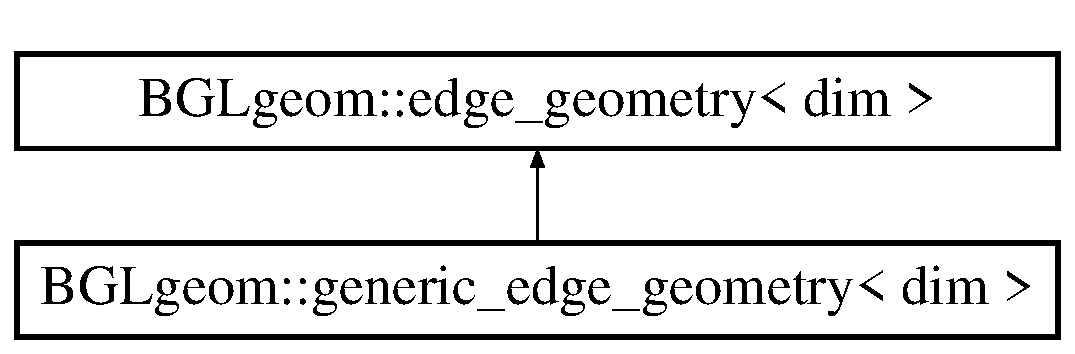
\includegraphics[height=2cm]{classBGLgeom_1_1generic__edge__geometry}
\end{center}
\end{figure}
\subsection*{Public Member Functions}
\begin{DoxyCompactItemize}
\item 
\hyperlink{classBGLgeom_1_1generic__edge__geometry_abc3ee901035797edb931ca75f3dbbdcf}{generic\_\-edge\_\-geometry} (std::function$<$ \hyperlink{classBGLgeom_1_1point}{BGLgeom::point}$<$ dim $>$(double)$>$ value\_\-)
\begin{DoxyCompactList}\small\item\em s:\mbox{[}0,1\mbox{]} -\/$>$ value\_\-fun(s):\mbox{[}0,1\mbox{]}$^\wedge$dim \item\end{DoxyCompactList}\item 
\hypertarget{classBGLgeom_1_1generic__edge__geometry_abf3bcb08edce314687a102a814899e9c}{
\hyperlink{classBGLgeom_1_1generic__edge__geometry_abf3bcb08edce314687a102a814899e9c}{generic\_\-edge\_\-geometry} ()}
\label{classBGLgeom_1_1generic__edge__geometry_abf3bcb08edce314687a102a814899e9c}

\begin{DoxyCompactList}\small\item\em default constructor: linear edge (oppure defaultizzo già il fatto di chiamare sempre il linear\_\-edge se non altrimenti specificato?) \item\end{DoxyCompactList}\item 
virtual std::vector$<$ double $>$ \hyperlink{classBGLgeom_1_1generic__edge__geometry_ad9052ef00b87b9f8ef26a3944ba5e43c}{first\_\-derivatives} (const double x)
\begin{DoxyCompactList}\small\item\em first derivative \item\end{DoxyCompactList}\item 
\hypertarget{classBGLgeom_1_1generic__edge__geometry_a92bb8e77f6d642017313d828123f2907}{
virtual std::vector$<$ double $>$ \hyperlink{classBGLgeom_1_1generic__edge__geometry_a92bb8e77f6d642017313d828123f2907}{second\_\-derivatives} (const double x)}
\label{classBGLgeom_1_1generic__edge__geometry_a92bb8e77f6d642017313d828123f2907}

\begin{DoxyCompactList}\small\item\em second derivative \item\end{DoxyCompactList}\item 
virtual \hyperlink{classBGLgeom_1_1point}{BGLgeom::point}$<$ dim $>$ \hyperlink{classBGLgeom_1_1generic__edge__geometry_a7bb600748e2b9aef8bf8bcb1bb5fec6e}{value} (const double parameter)
\begin{DoxyCompactList}\small\item\em curvilinear abscissa \item\end{DoxyCompactList}\end{DoxyCompactItemize}
\subsubsection*{template$<$unsigned int dim$>$ class BGLgeom::generic\_\-edge\_\-geometry$<$ dim $>$}



\subsection{Constructor \& Destructor Documentation}
\hypertarget{classBGLgeom_1_1generic__edge__geometry_abc3ee901035797edb931ca75f3dbbdcf}{
\index{BGLgeom::generic\_\-edge\_\-geometry@{BGLgeom::generic\_\-edge\_\-geometry}!generic\_\-edge\_\-geometry@{generic\_\-edge\_\-geometry}}
\index{generic\_\-edge\_\-geometry@{generic\_\-edge\_\-geometry}!BGLgeom::generic_edge_geometry@{BGLgeom::generic\_\-edge\_\-geometry}}
\subsubsection[{generic\_\-edge\_\-geometry}]{\setlength{\rightskip}{0pt plus 5cm}template$<$unsigned int dim$>$ {\bf BGLgeom::generic\_\-edge\_\-geometry}$<$ dim $>$::{\bf generic\_\-edge\_\-geometry} (std::function$<$ {\bf BGLgeom::point}$<$ dim $>$(double)$>$ {\em value\_\-})\hspace{0.3cm}{\ttfamily  \mbox{[}inline\mbox{]}}}}
\label{classBGLgeom_1_1generic__edge__geometry_abc3ee901035797edb931ca75f3dbbdcf}


s:\mbox{[}0,1\mbox{]} -\/$>$ value\_\-fun(s):\mbox{[}0,1\mbox{]}$^\wedge$dim stores the function which takes in input the \char`\"{}normalized\char`\"{} parametrization of the edge constructor 

\subsection{Member Function Documentation}
\hypertarget{classBGLgeom_1_1generic__edge__geometry_ad9052ef00b87b9f8ef26a3944ba5e43c}{
\index{BGLgeom::generic\_\-edge\_\-geometry@{BGLgeom::generic\_\-edge\_\-geometry}!first\_\-derivatives@{first\_\-derivatives}}
\index{first\_\-derivatives@{first\_\-derivatives}!BGLgeom::generic_edge_geometry@{BGLgeom::generic\_\-edge\_\-geometry}}
\subsubsection[{first\_\-derivatives}]{\setlength{\rightskip}{0pt plus 5cm}template$<$unsigned int dim$>$ virtual std::vector$<$double$>$ {\bf BGLgeom::generic\_\-edge\_\-geometry}$<$ dim $>$::first\_\-derivatives (const double {\em x})\hspace{0.3cm}{\ttfamily  \mbox{[}inline, virtual\mbox{]}}}}
\label{classBGLgeom_1_1generic__edge__geometry_ad9052ef00b87b9f8ef26a3944ba5e43c}


first derivative 

declare the \hyperlink{classBGLgeom_1_1point}{point} that will contain the result 

Implements \hyperlink{classBGLgeom_1_1edge__geometry}{BGLgeom::edge\_\-geometry$<$ dim $>$}.\hypertarget{classBGLgeom_1_1generic__edge__geometry_a7bb600748e2b9aef8bf8bcb1bb5fec6e}{
\index{BGLgeom::generic\_\-edge\_\-geometry@{BGLgeom::generic\_\-edge\_\-geometry}!value@{value}}
\index{value@{value}!BGLgeom::generic_edge_geometry@{BGLgeom::generic\_\-edge\_\-geometry}}
\subsubsection[{value}]{\setlength{\rightskip}{0pt plus 5cm}template$<$unsigned int dim$>$ virtual {\bf BGLgeom::point}$<$dim$>$ {\bf BGLgeom::generic\_\-edge\_\-geometry}$<$ dim $>$::value (const double {\em parameter})\hspace{0.3cm}{\ttfamily  \mbox{[}inline, virtual\mbox{]}}}}
\label{classBGLgeom_1_1generic__edge__geometry_a7bb600748e2b9aef8bf8bcb1bb5fec6e}


curvilinear abscissa returns value fun (parametrized between 0 and 1) in s between 0 and 1 

Implements \hyperlink{classBGLgeom_1_1edge__geometry}{BGLgeom::edge\_\-geometry$<$ dim $>$}.

The documentation for this class was generated from the following file:\begin{DoxyCompactItemize}
\item 
include/\hyperlink{generic__edge__geometry_8hpp}{generic\_\-edge\_\-geometry.hpp}\end{DoxyCompactItemize}

\hypertarget{structGeometry_1_1Intersection}{
\section{Geometry::Intersection Struct Reference}
\label{structGeometry_1_1Intersection}\index{Geometry::Intersection@{Geometry::Intersection}}
}


A simple struct that contains the result of the intersection test.  


{\ttfamily \#include $<$intersector\_\-base\_\-class.hpp$>$}\subsection*{Public Attributes}
\begin{DoxyCompactItemize}
\item 
bool \hyperlink{structGeometry_1_1Intersection_a45563c77f618ad3a58931ed051032d45}{intersect} = false
\begin{DoxyCompactList}\small\item\em Segments intersects. \item\end{DoxyCompactList}\item 
\hypertarget{structGeometry_1_1Intersection_a30339c7930808caca3df89da3df2b034}{
unsigned int \hyperlink{structGeometry_1_1Intersection_a30339c7930808caca3df89da3df2b034}{numberOfIntersections} = 0u}
\label{structGeometry_1_1Intersection_a30339c7930808caca3df89da3df2b034}

\begin{DoxyCompactList}\small\item\em Number of intersections (max 2). \item\end{DoxyCompactList}\item 
\hypertarget{structGeometry_1_1Intersection_abd19dce0869cb0e34ce94f48138b8f38}{
std::array$<$ point$<$ 2 $>$, 2 $>$ \hyperlink{structGeometry_1_1Intersection_abd19dce0869cb0e34ce94f48138b8f38}{intersectionPoint} = std::array$<$point$<$2$>$,2$>$\{point$<$2$>$(), point$<$2$>$()\}}
\label{structGeometry_1_1Intersection_abd19dce0869cb0e34ce94f48138b8f38}

\begin{DoxyCompactList}\small\item\em \hyperlink{structGeometry_1_1Intersection}{Intersection} points coordinates. \item\end{DoxyCompactList}\item 
std::array$<$ std::array$<$ bool, 2 $>$, 2 $>$ \hyperlink{structGeometry_1_1Intersection_ac26994bdf89460be8b13c1304796b6bb}{endPointIsIntersection}
\item 
std::array$<$ std::array$<$ int, 2 $>$, 2 $>$ \hyperlink{structGeometry_1_1Intersection_a15cd54d14fc1ddc1f4499dc49e1d5508}{otherEdgePoint}
\item 
\hypertarget{structGeometry_1_1Intersection_aad30a67c865aca570fff7f29a9251903}{
bool \hyperlink{structGeometry_1_1Intersection_aad30a67c865aca570fff7f29a9251903}{parallel} = false}
\label{structGeometry_1_1Intersection_aad30a67c865aca570fff7f29a9251903}

\begin{DoxyCompactList}\small\item\em Edges are parallel. \item\end{DoxyCompactList}\item 
\hypertarget{structGeometry_1_1Intersection_a3a5657af0debf92f5653e1f7627ce417}{
bool \hyperlink{structGeometry_1_1Intersection_a3a5657af0debf92f5653e1f7627ce417}{identical} = false}
\label{structGeometry_1_1Intersection_a3a5657af0debf92f5653e1f7627ce417}

\begin{DoxyCompactList}\small\item\em Edges are identical. \item\end{DoxyCompactList}\item 
\hypertarget{structGeometry_1_1Intersection_a468bd7fe9703f6bd57aabbd0d957668e}{
bool \hyperlink{structGeometry_1_1Intersection_a468bd7fe9703f6bd57aabbd0d957668e}{collinear} = false}
\label{structGeometry_1_1Intersection_a468bd7fe9703f6bd57aabbd0d957668e}

\begin{DoxyCompactList}\small\item\em Edges are collinear (and thus also parallel). \item\end{DoxyCompactList}\item 
\hypertarget{structGeometry_1_1Intersection_adde469457ed9ef6a0a9df12d5c5be23f}{
bool \hyperlink{structGeometry_1_1Intersection_adde469457ed9ef6a0a9df12d5c5be23f}{good} = true}
\label{structGeometry_1_1Intersection_adde469457ed9ef6a0a9df12d5c5be23f}

\begin{DoxyCompactList}\small\item\em Something is not ok. \item\end{DoxyCompactList}\item 
\hypertarget{structGeometry_1_1Intersection_a08f4c2d8a818d21883e35c932088b6ed}{
double \hyperlink{structGeometry_1_1Intersection_a08f4c2d8a818d21883e35c932088b6ed}{distance} = 0.0}
\label{structGeometry_1_1Intersection_a08f4c2d8a818d21883e35c932088b6ed}

\begin{DoxyCompactList}\small\item\em Distance, makes sense only if parallel=true. \item\end{DoxyCompactList}\end{DoxyCompactItemize}


\subsection{Detailed Description}
A simple struct that contains the result of the intersection test. To be able to treat the most general case each segment is allowed to have up to two intersections. It happens if the segments overlaps

\begin{Desc}
\item[\hyperlink{todo__todo000001}{Todo}]It can be bettered by adding another attribute that indicates, in the case of two edges end which coincides the relative position on the edge. It requires a simple modification of the function segmentIntersect \end{Desc}
\begin{DoxyNote}{Note}
Piece of code provided by prof. Formaggia 
\end{DoxyNote}


\subsection{Member Data Documentation}
\hypertarget{structGeometry_1_1Intersection_ac26994bdf89460be8b13c1304796b6bb}{
\index{Geometry::Intersection@{Geometry::Intersection}!endPointIsIntersection@{endPointIsIntersection}}
\index{endPointIsIntersection@{endPointIsIntersection}!Geometry::Intersection@{Geometry::Intersection}}
\subsubsection[{endPointIsIntersection}]{\setlength{\rightskip}{0pt plus 5cm}std::array$<$std::array$<$bool,2$>$, 2$>$ {\bf Geometry::Intersection::endPointIsIntersection}}}
\label{structGeometry_1_1Intersection_ac26994bdf89460be8b13c1304796b6bb}
{\bfseries Initial value:}
\begin{DoxyCode}

            std::array<std::array<bool,2>, 2>{std::array<bool,2>{false,false}, st
      d::array<bool,2>{false,false} }
\end{DoxyCode}
\hyperlink{structGeometry_1_1Intersection}{Intersection} may be end point

endPointIsIntersection\mbox{[}i\mbox{]}\mbox{[}j\mbox{]}=true then end j of edge i is at the intersection \hypertarget{structGeometry_1_1Intersection_a45563c77f618ad3a58931ed051032d45}{
\index{Geometry::Intersection@{Geometry::Intersection}!intersect@{intersect}}
\index{intersect@{intersect}!Geometry::Intersection@{Geometry::Intersection}}
\subsubsection[{intersect}]{\setlength{\rightskip}{0pt plus 5cm}bool {\bf Geometry::Intersection::intersect} = false}}
\label{structGeometry_1_1Intersection_a45563c77f618ad3a58931ed051032d45}


Segments intersects. True is there is any intersection \hypertarget{structGeometry_1_1Intersection_a15cd54d14fc1ddc1f4499dc49e1d5508}{
\index{Geometry::Intersection@{Geometry::Intersection}!otherEdgePoint@{otherEdgePoint}}
\index{otherEdgePoint@{otherEdgePoint}!Geometry::Intersection@{Geometry::Intersection}}
\subsubsection[{otherEdgePoint}]{\setlength{\rightskip}{0pt plus 5cm}std::array$<$std::array$<$int,2$>$, 2$>$ {\bf Geometry::Intersection::otherEdgePoint}}}
\label{structGeometry_1_1Intersection_a15cd54d14fc1ddc1f4499dc49e1d5508}
{\bfseries Initial value:}
\begin{DoxyCode}

            std::array<std::array<int,2>, 2>{std::array<int,2>{-1,-1}, std::array
      <int,2>{-1,-1}}
\end{DoxyCode}
EdgeS join at the end. In that case endPointIsIntersection will be true and the corresponding entry will indicate the numering of the end of the other edge. -\/1 indicates that the end is not joined. So if endPointIsIntersection\mbox{[}i\mbox{]}\mbox{[}j\mbox{]}=true we have otherEdgePoint\mbox{[}i\mbox{]}\mbox{[}j\mbox{]}=-\/1 //End point is not joined with the other edge otherEdgePoint\mbox{[}i\mbox{]}\mbox{[}j\mbox{]}= k //End point j of edge j is joined with end point k of other edge 

The documentation for this struct was generated from the following file:\begin{DoxyCompactItemize}
\item 
include/\hyperlink{intersector__base__class_8hpp}{intersector\_\-base\_\-class.hpp}\end{DoxyCompactItemize}

\hypertarget{classintersector__base__class}{
\section{intersector\_\-base\_\-class$<$ Graph $>$ Class Template Reference}
\label{classintersector__base__class}\index{intersector\_\-base\_\-class@{intersector\_\-base\_\-class}}
}
Inheritance diagram for intersector\_\-base\_\-class$<$ Graph $>$::\begin{figure}[H]
\begin{center}
\leavevmode
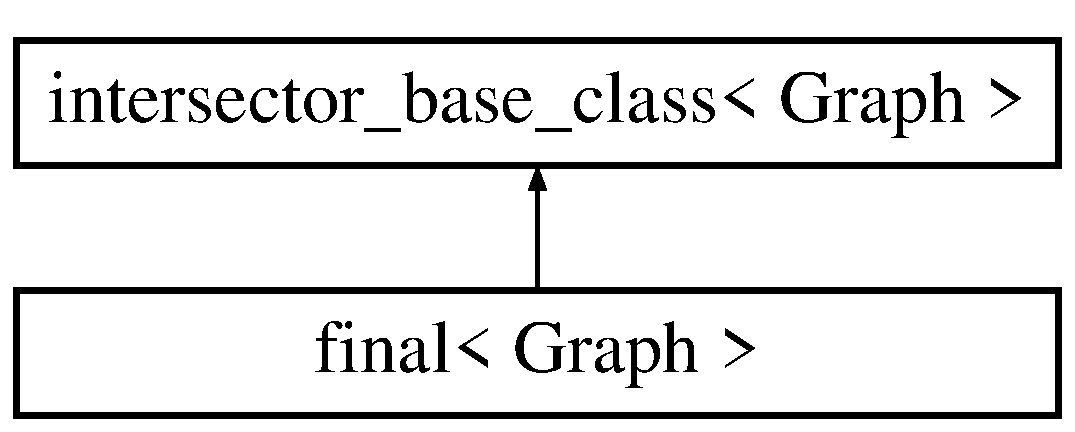
\includegraphics[height=2cm]{classintersector__base__class}
\end{center}
\end{figure}
\subsection*{Public Types}
\begin{DoxyCompactItemize}
\item 
\hypertarget{classintersector__base__class_aa920b0069f7bbbcfc63ff414e5fb40e7}{
typedef boost::graph\_\-traits$<$ Graph $>$::edge\_\-descriptor {\bfseries Edge\_\-desc}}
\label{classintersector__base__class_aa920b0069f7bbbcfc63ff414e5fb40e7}

\item 
\hypertarget{classintersector__base__class_a5a2f61f96a7efaef6f91fa743a799a9a}{
typedef boost::graph\_\-traits$<$ Graph $>$::edge\_\-iterator {\bfseries Edge\_\-iter}}
\label{classintersector__base__class_a5a2f61f96a7efaef6f91fa743a799a9a}

\item 
\hypertarget{classintersector__base__class_a197f03d7b72cd9fb141e619e3604da05}{
typedef boost::graph\_\-traits$<$ Graph $>$::vertex\_\-descriptor {\bfseries Vertex\_\-desc}}
\label{classintersector__base__class_a197f03d7b72cd9fb141e619e3604da05}

\item 
\hypertarget{classintersector__base__class_a11ff6c047c7579ba8da998a38b62f092}{
typedef std::pair$<$ point$<$ 2 $>$, point$<$ 2 $>$ $>$ {\bfseries Line}}
\label{classintersector__base__class_a11ff6c047c7579ba8da998a38b62f092}

\item 
\hypertarget{classintersector__base__class_aeead4d06ad6300f189924f29bc15e0d4}{
typedef std::vector$<$ std::pair$<$ point$<$ 2 $>$, Edge\_\-desc $>$ $>$ {\bfseries Intersections\_\-type}}
\label{classintersector__base__class_aeead4d06ad6300f189924f29bc15e0d4}

\item 
\hypertarget{classintersector__base__class_abf991566a0fca9f2601f028ead8890ea}{
typedef std::pair$<$ point$<$ 2 $>$, Edge\_\-desc $>$ {\bfseries Intersections\_\-value\_\-type}}
\label{classintersector__base__class_abf991566a0fca9f2601f028ead8890ea}

\end{DoxyCompactItemize}
\subsection*{Public Member Functions}
\begin{DoxyCompactItemize}
\item 
\hypertarget{classintersector__base__class_a8d13a4f8f6dec439866977a5b4fb0795}{
\hyperlink{classintersector__base__class_a8d13a4f8f6dec439866977a5b4fb0795}{intersector\_\-base\_\-class} ()}
\label{classintersector__base__class_a8d13a4f8f6dec439866977a5b4fb0795}

\begin{DoxyCompactList}\small\item\em Default constructor (initialization of the reference to the graph needed). \item\end{DoxyCompactList}\item 
\hypertarget{classintersector__base__class_a76525dba7cbd3b4d291281f71b2d1723}{
\hyperlink{classintersector__base__class_a76525dba7cbd3b4d291281f71b2d1723}{intersector\_\-base\_\-class} (\hyperlink{classintersector__base__class}{intersector\_\-base\_\-class} const \&)}
\label{classintersector__base__class_a76525dba7cbd3b4d291281f71b2d1723}

\begin{DoxyCompactList}\small\item\em Copy constructor. \item\end{DoxyCompactList}\item 
\hypertarget{classintersector__base__class_aeca93030cff57166c7b70b2911a7bddf}{
virtual \hyperlink{classintersector__base__class_aeca93030cff57166c7b70b2911a7bddf}{$\sim$intersector\_\-base\_\-class} ()}
\label{classintersector__base__class_aeca93030cff57166c7b70b2911a7bddf}

\begin{DoxyCompactList}\small\item\em Destructor. \item\end{DoxyCompactList}\item 
\hypertarget{classintersector__base__class_a3486613036aada6bf7174f158282649b}{
\hyperlink{classintersector__base__class}{intersector\_\-base\_\-class} \& \hyperlink{classintersector__base__class_a3486613036aada6bf7174f158282649b}{operator=} (\hyperlink{classintersector__base__class}{intersector\_\-base\_\-class} const \&)}
\label{classintersector__base__class_a3486613036aada6bf7174f158282649b}

\begin{DoxyCompactList}\small\item\em Assignment operator. \item\end{DoxyCompactList}\item 
\hypertarget{classintersector__base__class_a6c8fee82915c3745f41ffb5b714bda1c}{
virtual void \hyperlink{classintersector__base__class_a6c8fee82915c3745f41ffb5b714bda1c}{set\_\-Edge1} (point$<$ 2 $>$ const \&P1, point$<$ 2 $>$ const \&P2)}
\label{classintersector__base__class_a6c8fee82915c3745f41ffb5b714bda1c}

\begin{DoxyCompactList}\small\item\em It sets Edge1 from two points. \item\end{DoxyCompactList}\item 
\hypertarget{classintersector__base__class_a789a58d61926fc4f2b5fc096f355633b}{
virtual void \hyperlink{classintersector__base__class_a789a58d61926fc4f2b5fc096f355633b}{set\_\-Edge1} (Line \_\-L)}
\label{classintersector__base__class_a789a58d61926fc4f2b5fc096f355633b}

\begin{DoxyCompactList}\small\item\em It sets Edge1 from another Line. \item\end{DoxyCompactList}\item 
\hypertarget{classintersector__base__class_a60fe2748b57d0004d51e2ab0d8499401}{
virtual void \hyperlink{classintersector__base__class_a60fe2748b57d0004d51e2ab0d8499401}{set\_\-Edge2} (point$<$ 2 $>$ const \&P1, point$<$ 2 $>$ const \&P2)}
\label{classintersector__base__class_a60fe2748b57d0004d51e2ab0d8499401}

\begin{DoxyCompactList}\small\item\em It sets Edge2 from two points. \item\end{DoxyCompactList}\item 
\hypertarget{classintersector__base__class_a9388c8ba39f252ce90ba27958c212bdc}{
virtual void \hyperlink{classintersector__base__class_a9388c8ba39f252ce90ba27958c212bdc}{set\_\-Edge2} (Line \_\-L)}
\label{classintersector__base__class_a9388c8ba39f252ce90ba27958c212bdc}

\begin{DoxyCompactList}\small\item\em It sets Edge1 from another Line. \item\end{DoxyCompactList}\item 
\hypertarget{classintersector__base__class_ae7956127e010d767ade9529a977ac860}{
virtual void \hyperlink{classintersector__base__class_ae7956127e010d767ade9529a977ac860}{set\_\-Edge2\_\-descriptor} (Edge\_\-desc \_\-Edge2\_\-desc)}
\label{classintersector__base__class_ae7956127e010d767ade9529a977ac860}

\begin{DoxyCompactList}\small\item\em It allows to set Edge2\_\-descriptor. \item\end{DoxyCompactList}\item 
\hypertarget{classintersector__base__class_a228d28f80f13bf02b88f02a8d015c6a0}{
virtual bool \hyperlink{classintersector__base__class_a228d28f80f13bf02b88f02a8d015c6a0}{are\_\-intersected} ()=0}
\label{classintersector__base__class_a228d28f80f13bf02b88f02a8d015c6a0}

\begin{DoxyCompactList}\small\item\em It checks if Edge1 and Edge2 are actually intersected  If the two edge are intersecating, this method must store in the class variable intersection\_\-point the coordinates of the intersection found. \item\end{DoxyCompactList}\item 
\hypertarget{classintersector__base__class_aac491cba39ea4dc1abe943a007b62de9}{
virtual void \hyperlink{classintersector__base__class_aac491cba39ea4dc1abe943a007b62de9}{store\_\-intersection} ()}
\label{classintersector__base__class_aac491cba39ea4dc1abe943a007b62de9}

\begin{DoxyCompactList}\small\item\em It pushes back a new intersection point between Edge1 and Edge2, remembering the edge descriptor of Edge2. \item\end{DoxyCompactList}\item 
\hypertarget{classintersector__base__class_a4ea6e2420f0a43f8f5066371e2efc1a5}{
virtual void {\bfseries clear\_\-intersections} ()}
\label{classintersector__base__class_a4ea6e2420f0a43f8f5066371e2efc1a5}

\item 
\hypertarget{classintersector__base__class_a50ea9691038f34ac8dae9f80af5e8fb6}{
virtual void \hyperlink{classintersector__base__class_a50ea9691038f34ac8dae9f80af5e8fb6}{refine\_\-graph} ()=0}
\label{classintersector__base__class_a50ea9691038f34ac8dae9f80af5e8fb6}

\begin{DoxyCompactList}\small\item\em It explains how to rebuilt graph after the intersections were computed  It has to inteface with private attributes of the derived class in order to set edge and vertex properties in the right way. \item\end{DoxyCompactList}\item 
\hypertarget{classintersector__base__class_ac7266d33ff6840e07837ed3247ef3de7}{
virtual void \hyperlink{classintersector__base__class_ac7266d33ff6840e07837ed3247ef3de7}{order\_\-intersections} ()=0}
\label{classintersector__base__class_ac7266d33ff6840e07837ed3247ef3de7}

\begin{DoxyCompactList}\small\item\em This reorders the vector intersections according to some order, defined by the user  It will consist of a call to \char`\"{}sort\char`\"{} algorithm, in which the compare function must be user defined, choosing a possible ordering in the 2D space. \item\end{DoxyCompactList}\end{DoxyCompactItemize}
\subsection*{Protected Attributes}
\begin{DoxyCompactItemize}
\item 
\hypertarget{classintersector__base__class_a9d52bda5a4eae76968f8cac57d055c41}{
Line \hyperlink{classintersector__base__class_a9d52bda5a4eae76968f8cac57d055c41}{Edge1}}
\label{classintersector__base__class_a9d52bda5a4eae76968f8cac57d055c41}

\begin{DoxyCompactList}\small\item\em The first of the two edge that are (maybe) intersecating  If the user has to perform multiple intersection between a fixed edge and all the other edges in the graph, Edge1 is thougth to be the fixed edge. \item\end{DoxyCompactList}\item 
\hypertarget{classintersector__base__class_af568953d08cce423eda95e4a7fbe1ecf}{
Line \hyperlink{classintersector__base__class_af568953d08cce423eda95e4a7fbe1ecf}{Edge2}}
\label{classintersector__base__class_af568953d08cce423eda95e4a7fbe1ecf}

\begin{DoxyCompactList}\small\item\em The second of the two edge that are (maybe) intersecating  If the user has to perform multiple intersection between a fixed edge and all the other edges in the graph, Edge2 is thougth to be the variable edge. \item\end{DoxyCompactList}\item 
\hypertarget{classintersector__base__class_a519ee3535c9e7aaf97a547413ebe0b08}{
Intersections\_\-type \hyperlink{classintersector__base__class_a519ee3535c9e7aaf97a547413ebe0b08}{intersections}}
\label{classintersector__base__class_a519ee3535c9e7aaf97a547413ebe0b08}

\begin{DoxyCompactList}\small\item\em Vector that will contains the intersection point and the edge descriptor of the edge with which the current edge is intersecating. \item\end{DoxyCompactList}\item 
\hypertarget{classintersector__base__class_a13c90acea49e8fef960046229a68e8b6}{
point$<$ 2 $>$ \hyperlink{classintersector__base__class_a13c90acea49e8fef960046229a68e8b6}{intersection\_\-point}}
\label{classintersector__base__class_a13c90acea49e8fef960046229a68e8b6}

\begin{DoxyCompactList}\small\item\em The intersection point between Edge1 and Edge2 (if present). \item\end{DoxyCompactList}\item 
\hypertarget{classintersector__base__class_a87fabe1d84ba485f04a46d5202e7bf23}{
Edge\_\-desc \hyperlink{classintersector__base__class_a87fabe1d84ba485f04a46d5202e7bf23}{Edge2\_\-descriptor}}
\label{classintersector__base__class_a87fabe1d84ba485f04a46d5202e7bf23}

\begin{DoxyCompactList}\small\item\em Edge descriptor of Edge2.  If the user has to perform multiple intersections between Edge1 (fixed) and Edge2 (variable), this tracks the edge descriptor of the edges in the graph that are intersecating Edge1 (one at a time). \item\end{DoxyCompactList}\end{DoxyCompactItemize}
\subsubsection*{template$<$typename Graph$>$ class intersector\_\-base\_\-class$<$ Graph $>$}



The documentation for this class was generated from the following file:\begin{DoxyCompactItemize}
\item 
include/\hyperlink{intersector__base__class_8hpp}{intersector\_\-base\_\-class.hpp}\end{DoxyCompactItemize}

\hypertarget{classGeometry_1_1Linear__edge}{
\section{Geometry::Linear\_\-edge Class Reference}
\label{classGeometry_1_1Linear__edge}\index{Geometry::Linear\_\-edge@{Geometry::Linear\_\-edge}}
}


A simple class that hanlde a linear edge  This class is thought to manage the description of the geometry of a linear edge, in order to compute intersections.  


{\ttfamily \#include $<$intersector\_\-base\_\-class.hpp$>$}\subsection*{Public Member Functions}
\begin{DoxyCompactItemize}
\item 
\hypertarget{classGeometry_1_1Linear__edge_a7bc8e67881017b2f3a60b513f81aa45f}{
\hyperlink{classGeometry_1_1Linear__edge_a7bc8e67881017b2f3a60b513f81aa45f}{Linear\_\-edge} ()}
\label{classGeometry_1_1Linear__edge_a7bc8e67881017b2f3a60b513f81aa45f}

\begin{DoxyCompactList}\small\item\em Default constructor. \item\end{DoxyCompactList}\item 
\hypertarget{classGeometry_1_1Linear__edge_a2a06df3a5dcb107522b4cafb8b1794d2}{
{\bfseries extremes\_\-are\_\-set} (false)}
\label{classGeometry_1_1Linear__edge_a2a06df3a5dcb107522b4cafb8b1794d2}

\item 
\hypertarget{classGeometry_1_1Linear__edge_ac3cb6d63d81f758cae11b315c81acc6e}{
\hyperlink{classGeometry_1_1Linear__edge_ac3cb6d63d81f758cae11b315c81acc6e}{Linear\_\-edge} (point$<$ 2 $>$ const \&SRC, point$<$ 2 $>$ const \&TGT)}
\label{classGeometry_1_1Linear__edge_ac3cb6d63d81f758cae11b315c81acc6e}

\begin{DoxyCompactList}\small\item\em Constructor. \item\end{DoxyCompactList}\item 
\hypertarget{classGeometry_1_1Linear__edge_a6f209351de4a6d48f16f01ca7fd72633}{
{\bfseries extremes\_\-are\_\-set} (true)}
\label{classGeometry_1_1Linear__edge_a6f209351de4a6d48f16f01ca7fd72633}

\item 
\hypertarget{classGeometry_1_1Linear__edge_af3a8b762ff05d8db1a3c976e2985ebb2}{
\hyperlink{classGeometry_1_1Linear__edge_af3a8b762ff05d8db1a3c976e2985ebb2}{Linear\_\-edge} (\hyperlink{classGeometry_1_1Linear__edge}{Linear\_\-edge} const \&)}
\label{classGeometry_1_1Linear__edge_af3a8b762ff05d8db1a3c976e2985ebb2}

\begin{DoxyCompactList}\small\item\em Copy constructor. \item\end{DoxyCompactList}\item 
\hypertarget{classGeometry_1_1Linear__edge_ab1cab14e36cf0e1d51bc68dea4c736a3}{
\hyperlink{classGeometry_1_1Linear__edge}{Linear\_\-edge} \& \hyperlink{classGeometry_1_1Linear__edge_ab1cab14e36cf0e1d51bc68dea4c736a3}{operator=} (\hyperlink{classGeometry_1_1Linear__edge}{Linear\_\-edge} const \&)}
\label{classGeometry_1_1Linear__edge_ab1cab14e36cf0e1d51bc68dea4c736a3}

\begin{DoxyCompactList}\small\item\em Assignment operator. \item\end{DoxyCompactList}\item 
\hypertarget{classGeometry_1_1Linear__edge_a567dadf0feb7d130903b7d2aaebfdf08}{
void \hyperlink{classGeometry_1_1Linear__edge_a567dadf0feb7d130903b7d2aaebfdf08}{set} (point$<$ 2 $>$ const \&SRC, point$<$ 2 $>$ const \&TGT)}
\label{classGeometry_1_1Linear__edge_a567dadf0feb7d130903b7d2aaebfdf08}

\begin{DoxyCompactList}\small\item\em Setting the two end points (extremes) of the edge. \item\end{DoxyCompactList}\item 
\hypertarget{classGeometry_1_1Linear__edge_a93a04309b0e46c40eb803a60d213a527}{
point$<$ 2 $>$ \hyperlink{classGeometry_1_1Linear__edge_a93a04309b0e46c40eb803a60d213a527}{operator\mbox{[}$\,$\mbox{]}} (std::size\_\-t i)}
\label{classGeometry_1_1Linear__edge_a93a04309b0e46c40eb803a60d213a527}

\begin{DoxyCompactList}\small\item\em Overloading of operator\mbox{[}\mbox{]} to access each of the two end points. Usefull in algorithms  extremes\mbox{[}0\mbox{]} = source, extremes\mbox{[}1\mbox{]} = target of the edge. \item\end{DoxyCompactList}\item 
\hypertarget{classGeometry_1_1Linear__edge_ab575249c0388c9c335b3d121d98f27b3}{
point$<$ 2 $>$ {\bfseries operator\mbox{[}$\,$\mbox{]}} (std::size\_\-t i) const }
\label{classGeometry_1_1Linear__edge_ab575249c0388c9c335b3d121d98f27b3}

\end{DoxyCompactItemize}


\subsection{Detailed Description}
A simple class that hanlde a linear edge  This class is thought to manage the description of the geometry of a linear edge, in order to compute intersections. \begin{DoxyRemark}{Remarks}
The class must have an overload of operator\mbox{[}\mbox{]} in order to run in the function that computes intersections 
\end{DoxyRemark}


The documentation for this class was generated from the following file:\begin{DoxyCompactItemize}
\item 
include/\hyperlink{intersector__base__class_8hpp}{intersector\_\-base\_\-class.hpp}\end{DoxyCompactItemize}

\hypertarget{structmy__edge}{
\section{my\_\-edge Struct Reference}
\label{structmy__edge}\index{my\_\-edge@{my\_\-edge}}
}


The documentation for this struct was generated from the following file:\begin{DoxyCompactItemize}
\item 
include/\hyperlink{data__structure_8hpp}{data\_\-structure.hpp}\end{DoxyCompactItemize}

\hypertarget{classnew__reader__class}{
\section{new\_\-reader\_\-class$<$ Source\_\-data\_\-structure, Target\_\-data\_\-structure, Edge\_\-data\_\-structure, Topological\_\-data\_\-structure $>$ Class Template Reference}
\label{classnew__reader__class}\index{new\_\-reader\_\-class@{new\_\-reader\_\-class}}
}


Abstract class that implements the functionality to read a file and get data from it  The users has to specify, in the derived class, all variables he need in order to store information read from the input file. Then, through the definition of Edge\_\-data\_\-structure and Vertex\_\-data\_\-structure, he can get separately all the information to put on edges and vertices.  


{\ttfamily \#include $<$new\_\-reader\_\-class.hpp$>$}\subsection*{Public Member Functions}
\begin{DoxyCompactItemize}
\item 
\hypertarget{classnew__reader__class_ad011d88e27ee32447cd2427f526cc272}{
\hyperlink{classnew__reader__class_ad011d88e27ee32447cd2427f526cc272}{new\_\-reader\_\-class} ()}
\label{classnew__reader__class_ad011d88e27ee32447cd2427f526cc272}

\begin{DoxyCompactList}\small\item\em Default constructor. \item\end{DoxyCompactList}\item 
\hypertarget{classnew__reader__class_ad6c890b1812ba8191058350201e90059}{
\hyperlink{classnew__reader__class_ad6c890b1812ba8191058350201e90059}{new\_\-reader\_\-class} (std::string \_\-filename)}
\label{classnew__reader__class_ad6c890b1812ba8191058350201e90059}

\begin{DoxyCompactList}\small\item\em Constructor. \item\end{DoxyCompactList}\item 
\hypertarget{classnew__reader__class_ab07f8c95e1ce24bcf96bb875b80e0f54}{
\hyperlink{classnew__reader__class_ab07f8c95e1ce24bcf96bb875b80e0f54}{new\_\-reader\_\-class} (\hyperlink{classnew__reader__class}{new\_\-reader\_\-class} const \&)}
\label{classnew__reader__class_ab07f8c95e1ce24bcf96bb875b80e0f54}

\begin{DoxyCompactList}\small\item\em Copy constructor. \item\end{DoxyCompactList}\item 
\hyperlink{classnew__reader__class}{new\_\-reader\_\-class} \&\hyperlink{classnew__reader__class}{new\_\-reader\_\-class} const \&virtual void \hyperlink{classnew__reader__class_a7436b3cd7c184da759e645e446897b12}{set\_\-input} (std::string \_\-filename)
\begin{DoxyCompactList}\small\item\em Assignment operator. \item\end{DoxyCompactList}\item 
virtual void \hyperlink{classnew__reader__class_ae1d2a3f3688c63248728cdee111ff021}{ignore\_\-dummy\_\-lines} (unsigned int const \&n)
\begin{DoxyCompactList}\small\item\em Ignore n lines of the input code that the user knows he has not to read. \item\end{DoxyCompactList}\item 
\hypertarget{classnew__reader__class_a95f6bf521a51258b14e5b5755fe5e75f}{
virtual void \hyperlink{classnew__reader__class_a95f6bf521a51258b14e5b5755fe5e75f}{read\_\-line} ()}
\label{classnew__reader__class_a95f6bf521a51258b14e5b5755fe5e75f}

\begin{DoxyCompactList}\small\item\em Reads one line and put it into a istringstream. \item\end{DoxyCompactList}\item 
\hypertarget{classnew__reader__class_af9e0622ae0a6cd142d659dd9c23f4ed9}{
virtual bool \hyperlink{classnew__reader__class_af9e0622ae0a6cd142d659dd9c23f4ed9}{is\_\-eof} ()}
\label{classnew__reader__class_af9e0622ae0a6cd142d659dd9c23f4ed9}

\begin{DoxyCompactList}\small\item\em To know outside the class if we have reached the end of file. \item\end{DoxyCompactList}\item 
\hypertarget{classnew__reader__class_afca41f4c9ff70f55e93bdb17cd0b365a}{
virtual void \hyperlink{classnew__reader__class_afca41f4c9ff70f55e93bdb17cd0b365a}{get\_\-data\_\-from\_\-line} ()=0}
\label{classnew__reader__class_afca41f4c9ff70f55e93bdb17cd0b365a}

\begin{DoxyCompactList}\small\item\em Reads the data from one single line. It has to be specified by the user  It reads data form the istringstream iss\_\-line that is defined as an attribute of the class and it is updated after every call of \hyperlink{classnew__reader__class_a95f6bf521a51258b14e5b5755fe5e75f}{read\_\-line()}. \item\end{DoxyCompactList}\item 
\hypertarget{classnew__reader__class_ab01559704d4f1d609e732d77808b502e}{
virtual Edge\_\-data\_\-structure \hyperlink{classnew__reader__class_ab01559704d4f1d609e732d77808b502e}{get\_\-edge\_\-data} ()=0}
\label{classnew__reader__class_ab01559704d4f1d609e732d77808b502e}

\begin{DoxyCompactList}\small\item\em A method to get the right data to append to an edge. \item\end{DoxyCompactList}\item 
\hypertarget{classnew__reader__class_a572d6d26042e4b4d1f402ab0d350d06a}{
virtual Source\_\-data\_\-structure \hyperlink{classnew__reader__class_a572d6d26042e4b4d1f402ab0d350d06a}{get\_\-source\_\-data} ()=0}
\label{classnew__reader__class_a572d6d26042e4b4d1f402ab0d350d06a}

\begin{DoxyCompactList}\small\item\em A method to get the right data to append to the source. \item\end{DoxyCompactList}\item 
\hypertarget{classnew__reader__class_acc5596fe13aadce75d0dcb2554783b37}{
virtual Target\_\-data\_\-structure \hyperlink{classnew__reader__class_acc5596fe13aadce75d0dcb2554783b37}{get\_\-target\_\-data} ()=0}
\label{classnew__reader__class_acc5596fe13aadce75d0dcb2554783b37}

\begin{DoxyCompactList}\small\item\em A method to get the right data to append to the target. \item\end{DoxyCompactList}\item 
\hypertarget{classnew__reader__class_ae6355323cdaad87a64c01b8c0fdcff39}{
virtual Topological\_\-data\_\-structure \hyperlink{classnew__reader__class_ae6355323cdaad87a64c01b8c0fdcff39}{get\_\-topological\_\-data} ()=0}
\label{classnew__reader__class_ae6355323cdaad87a64c01b8c0fdcff39}

\begin{DoxyCompactList}\small\item\em A method to get the right topological data from a line. \item\end{DoxyCompactList}\end{DoxyCompactItemize}
\subsection*{Protected Attributes}
\begin{DoxyCompactItemize}
\item 
\hypertarget{classnew__reader__class_a9dcdd31bf0f8ae62cb7e5de0ef10c0f8}{
std::string \hyperlink{classnew__reader__class_a9dcdd31bf0f8ae62cb7e5de0ef10c0f8}{filename}}
\label{classnew__reader__class_a9dcdd31bf0f8ae62cb7e5de0ef10c0f8}

\begin{DoxyCompactList}\small\item\em The name of the file to be read. \item\end{DoxyCompactList}\item 
\hypertarget{classnew__reader__class_a015e6a646a92851042775e0211752a9e}{
std::ifstream \hyperlink{classnew__reader__class_a015e6a646a92851042775e0211752a9e}{in\_\-file}}
\label{classnew__reader__class_a015e6a646a92851042775e0211752a9e}

\begin{DoxyCompactList}\small\item\em File stream to handle the input file. \item\end{DoxyCompactList}\item 
\hypertarget{classnew__reader__class_a285a324c64b881c8cbcfb507c54af0bd}{
std::string \hyperlink{classnew__reader__class_a285a324c64b881c8cbcfb507c54af0bd}{line}}
\label{classnew__reader__class_a285a324c64b881c8cbcfb507c54af0bd}

\begin{DoxyCompactList}\small\item\em String in which the data read from a line are put. \item\end{DoxyCompactList}\item 
\hypertarget{classnew__reader__class_afd7ac3583e064f6164567d6b09c1d960}{
std::istringstream \hyperlink{classnew__reader__class_afd7ac3583e064f6164567d6b09c1d960}{iss\_\-line}}
\label{classnew__reader__class_afd7ac3583e064f6164567d6b09c1d960}

\begin{DoxyCompactList}\small\item\em Data put in line are converted in istringstream to be got by the user. \item\end{DoxyCompactList}\end{DoxyCompactItemize}


\subsection{Detailed Description}
\subsubsection*{template$<$typename Source\_\-data\_\-structure, typename Target\_\-data\_\-structure, typename Edge\_\-data\_\-structure, typename Topological\_\-data\_\-structure = no\_\-topological\_\-data$>$ class new\_\-reader\_\-class$<$ Source\_\-data\_\-structure, Target\_\-data\_\-structure, Edge\_\-data\_\-structure, Topological\_\-data\_\-structure $>$}

Abstract class that implements the functionality to read a file and get data from it  The users has to specify, in the derived class, all variables he need in order to store information read from the input file. Then, through the definition of Edge\_\-data\_\-structure and Vertex\_\-data\_\-structure, he can get separately all the information to put on edges and vertices. 
\begin{DoxyParams}{Parameters}
\item[{\em Edge\_\-data\_\-structure}]A struct where the user has to define type and name of the variables he needs to append to vertices as vertex bundled property \item[{\em Vertex\_\-data\_\-structure}]A struct where the user has to define type and name of the variables he needs to append to edge as edge bundled property \end{DoxyParams}
\begin{DoxyPrecond}{Precondition}
It may be useful to declare a friend operator$>$$>$ to help the reader read the data 
\end{DoxyPrecond}


\subsection{Member Function Documentation}
\hypertarget{classnew__reader__class_ae1d2a3f3688c63248728cdee111ff021}{
\index{new\_\-reader\_\-class@{new\_\-reader\_\-class}!ignore\_\-dummy\_\-lines@{ignore\_\-dummy\_\-lines}}
\index{ignore\_\-dummy\_\-lines@{ignore\_\-dummy\_\-lines}!new_reader_class@{new\_\-reader\_\-class}}
\subsubsection[{ignore\_\-dummy\_\-lines}]{\setlength{\rightskip}{0pt plus 5cm}template$<$typename Source\_\-data\_\-structure, typename Target\_\-data\_\-structure, typename Edge\_\-data\_\-structure, typename Topological\_\-data\_\-structure = no\_\-topological\_\-data$>$ virtual void {\bf new\_\-reader\_\-class}$<$ Source\_\-data\_\-structure, Target\_\-data\_\-structure, Edge\_\-data\_\-structure, Topological\_\-data\_\-structure $>$::ignore\_\-dummy\_\-lines (unsigned int const \& {\em n})\hspace{0.3cm}{\ttfamily  \mbox{[}inline, virtual\mbox{]}}}}
\label{classnew__reader__class_ae1d2a3f3688c63248728cdee111ff021}


Ignore n lines of the input code that the user knows he has not to read. \begin{DoxyRemark}{Remarks}
It sets the file stream n lines after the previous position 
\end{DoxyRemark}
\hypertarget{classnew__reader__class_a7436b3cd7c184da759e645e446897b12}{
\index{new\_\-reader\_\-class@{new\_\-reader\_\-class}!set\_\-input@{set\_\-input}}
\index{set\_\-input@{set\_\-input}!new_reader_class@{new\_\-reader\_\-class}}
\subsubsection[{set\_\-input}]{\setlength{\rightskip}{0pt plus 5cm}template$<$typename Source\_\-data\_\-structure, typename Target\_\-data\_\-structure, typename Edge\_\-data\_\-structure, typename Topological\_\-data\_\-structure = no\_\-topological\_\-data$>$ {\bf new\_\-reader\_\-class}\& {\bf new\_\-reader\_\-class} const\& virtual void {\bf new\_\-reader\_\-class}$<$ Source\_\-data\_\-structure, Target\_\-data\_\-structure, Edge\_\-data\_\-structure, Topological\_\-data\_\-structure $>$::set\_\-input (std::string {\em \_\-filename})\hspace{0.3cm}{\ttfamily  \mbox{[}inline, virtual\mbox{]}}}}
\label{classnew__reader__class_a7436b3cd7c184da759e645e446897b12}


Assignment operator. Set the input file to read 

The documentation for this class was generated from the following file:\begin{DoxyCompactItemize}
\item 
include/\hyperlink{new__reader__class_8hpp}{new\_\-reader\_\-class.hpp}\end{DoxyCompactItemize}

\hypertarget{structno__topological__data}{
\section{no\_\-topological\_\-data Struct Reference}
\label{structno__topological__data}\index{no\_\-topological\_\-data@{no\_\-topological\_\-data}}
}


An empty struct to handle the case the user do not need to store topological data  Inside this the user may put data as vertex and edge descriptor for the connettivity of the graph.  


{\ttfamily \#include $<$new\_\-reader\_\-class.hpp$>$}

\subsection{Detailed Description}
An empty struct to handle the case the user do not need to store topological data  Inside this the user may put data as vertex and edge descriptor for the connettivity of the graph. 

The documentation for this struct was generated from the following file:\begin{DoxyCompactItemize}
\item 
include/\hyperlink{new__reader__class_8hpp}{new\_\-reader\_\-class.hpp}\end{DoxyCompactItemize}

\hypertarget{classour__disjoint__sets}{
\section{our\_\-disjoint\_\-sets$<$ Graph $>$ Class Template Reference}
\label{classour__disjoint__sets}\index{our\_\-disjoint\_\-sets@{our\_\-disjoint\_\-sets}}
}


Template class to handle disjoint sets  The template parameters are:\par
 Label\_\-map\_\-t: the type of a std::map which key is a vertex descriptor and the value is an unsigned int which has the meaning of the current label of the component to which that vertex belongs to.\par
 Components\_\-map\_\-t: the type of a std::map which key is an unsigned int used as label for the group and the value is a std::set containing all the vertex descriptor of the vertices that have that label, i.e that belong to the same component.  


{\ttfamily \#include $<$our\_\-disjoint\_\-sets.hpp$>$}\subsection*{Public Types}
\begin{DoxyCompactItemize}
\item 
\hypertarget{classour__disjoint__sets_af331ecb5ad051216273fe2de9c4f3583}{
typedef boost::graph\_\-traits$<$ Graph $>$::vertex\_\-iterator {\bfseries Vertex\_\-iter}}
\label{classour__disjoint__sets_af331ecb5ad051216273fe2de9c4f3583}

\item 
\hypertarget{classour__disjoint__sets_a35cce28d3bc811993b9e880281745f0e}{
typedef boost::graph\_\-traits$<$ Graph $>$::vertex\_\-descriptor {\bfseries Vertex\_\-desc}}
\label{classour__disjoint__sets_a35cce28d3bc811993b9e880281745f0e}

\item 
\hypertarget{classour__disjoint__sets_a5e7555bfef19190e3c65f722024f2214}{
typedef std::map$<$ Vertex\_\-desc, unsigned int $>$ {\bfseries Label\_\-map\_\-t}}
\label{classour__disjoint__sets_a5e7555bfef19190e3c65f722024f2214}

\item 
\hypertarget{classour__disjoint__sets_a607a97b4454defc96ef7f684cbea3d83}{
typedef std::map$<$ unsigned int, std::list$<$ Vertex\_\-desc $>$ $>$ {\bfseries Components\_\-map\_\-t}}
\label{classour__disjoint__sets_a607a97b4454defc96ef7f684cbea3d83}

\item 
\hypertarget{classour__disjoint__sets_a79c7ea38049a78d9e74fbaa29edaa0a1}{
typedef Label\_\-map\_\-t::key\_\-type {\bfseries Label\_\-key\_\-t}}
\label{classour__disjoint__sets_a79c7ea38049a78d9e74fbaa29edaa0a1}

\item 
\hypertarget{classour__disjoint__sets_a686da13c5c36a0741ad28427e161578f}{
typedef Label\_\-map\_\-t::mapped\_\-type {\bfseries Label\_\-mapped\_\-t}}
\label{classour__disjoint__sets_a686da13c5c36a0741ad28427e161578f}

\item 
\hypertarget{classour__disjoint__sets_a752c86546f6ecbafbdeae7bf0a907c0e}{
typedef Components\_\-map\_\-t::key\_\-type {\bfseries Components\_\-key\_\-t}}
\label{classour__disjoint__sets_a752c86546f6ecbafbdeae7bf0a907c0e}

\item 
\hypertarget{classour__disjoint__sets_aa07b787857c3bcd01bbe9bf6f0bb5e94}{
typedef Components\_\-map\_\-t::mapped\_\-type {\bfseries Components\_\-mapped\_\-t}}
\label{classour__disjoint__sets_aa07b787857c3bcd01bbe9bf6f0bb5e94}

\item 
\hypertarget{classour__disjoint__sets_a510c748b30dafffd0ce483e9cdfae49b}{
typedef Components\_\-mapped\_\-t::value\_\-type {\bfseries Comp\_\-mapped\_\-vertex\_\-t}}
\label{classour__disjoint__sets_a510c748b30dafffd0ce483e9cdfae49b}

\end{DoxyCompactItemize}
\subsection*{Public Member Functions}
\begin{DoxyCompactItemize}
\item 
\hypertarget{classour__disjoint__sets_aa393efe7852a167a8134114122c3d4ce}{
\hyperlink{classour__disjoint__sets_aa393efe7852a167a8134114122c3d4ce}{our\_\-disjoint\_\-sets} (Graph \&\_\-G)}
\label{classour__disjoint__sets_aa393efe7852a167a8134114122c3d4ce}

\begin{DoxyCompactList}\small\item\em Default constructor. \item\end{DoxyCompactList}\item 
\hypertarget{classour__disjoint__sets_a7c887672236b2983a5e492f7f14cb183}{
\hyperlink{classour__disjoint__sets_a7c887672236b2983a5e492f7f14cb183}{our\_\-disjoint\_\-sets} (\hyperlink{classour__disjoint__sets}{our\_\-disjoint\_\-sets} const \&)}
\label{classour__disjoint__sets_a7c887672236b2983a5e492f7f14cb183}

\begin{DoxyCompactList}\small\item\em Copy constructor. \item\end{DoxyCompactList}\item 
\hypertarget{classour__disjoint__sets_a4985692effbfcd92fe0b4ed6776da712}{
\hyperlink{classour__disjoint__sets}{our\_\-disjoint\_\-sets} \& \hyperlink{classour__disjoint__sets_a4985692effbfcd92fe0b4ed6776da712}{operator=} (\hyperlink{classour__disjoint__sets}{our\_\-disjoint\_\-sets} const \&)}
\label{classour__disjoint__sets_a4985692effbfcd92fe0b4ed6776da712}

\begin{DoxyCompactList}\small\item\em Assignment operator. \item\end{DoxyCompactList}\item 
\hypertarget{classour__disjoint__sets_ac6753772c2b17555361b59826b4e3c35}{
\hyperlink{classour__disjoint__sets_ac6753772c2b17555361b59826b4e3c35}{$\sim$our\_\-disjoint\_\-sets} ()}
\label{classour__disjoint__sets_ac6753772c2b17555361b59826b4e3c35}

\begin{DoxyCompactList}\small\item\em Destructor. \item\end{DoxyCompactList}\item 
\hypertarget{classour__disjoint__sets_a94bb24df48460d40143758c9a4c3a7ef}{
void \hyperlink{classour__disjoint__sets_a94bb24df48460d40143758c9a4c3a7ef}{make\_\-label\_\-map} ()}
\label{classour__disjoint__sets_a94bb24df48460d40143758c9a4c3a7ef}

\begin{DoxyCompactList}\small\item\em It creates the label map starting form the Graph  The label\_\-map is set up by associating to each vertex descriptor a progressive unsigned int as label, that indicates to which component the vertex belongs to. In other words, label\_\-map is set up by assuming that each vertex is a separated component. \item\end{DoxyCompactList}\item 
\hypertarget{classour__disjoint__sets_a0735914ff4a2a87ec7ee261f1a132a49}{
Label\_\-mapped\_\-t \hyperlink{classour__disjoint__sets_a0735914ff4a2a87ec7ee261f1a132a49}{get\_\-label} (Label\_\-key\_\-t const \&vertex)}
\label{classour__disjoint__sets_a0735914ff4a2a87ec7ee261f1a132a49}

\begin{DoxyCompactList}\small\item\em It returns, from the label\_\-map, the label of the component which the vertex belongs to. \item\end{DoxyCompactList}\item 
\hypertarget{classour__disjoint__sets_a0db082ada0847dac4d5f017a1dae9cde}{
void \hyperlink{classour__disjoint__sets_a0db082ada0847dac4d5f017a1dae9cde}{set\_\-label} (Label\_\-key\_\-t const \&vertex, Label\_\-mapped\_\-t const \&label)}
\label{classour__disjoint__sets_a0db082ada0847dac4d5f017a1dae9cde}

\begin{DoxyCompactList}\small\item\em It allows to set the label of that vertex in label map. \item\end{DoxyCompactList}\item 
\hypertarget{classour__disjoint__sets_a7fc838875896a173f94134c5cdb5e0a1}{
bool \hyperlink{classour__disjoint__sets_a7fc838875896a173f94134c5cdb5e0a1}{is\_\-present\_\-component} (Components\_\-key\_\-t const \&label\_\-of\_\-the\_\-component)}
\label{classour__disjoint__sets_a7fc838875896a173f94134c5cdb5e0a1}

\begin{DoxyCompactList}\small\item\em Checks if a particular component (i.e its label) is already present in the components\_\-map. \item\end{DoxyCompactList}\item 
\hypertarget{classour__disjoint__sets_adb24c138a4220087fb93f6f8d7a6c17e}{
std::pair$<$ typename Components\_\-mapped\_\-t::iterator, typename Components\_\-mapped\_\-t::iterator $>$ \hyperlink{classour__disjoint__sets_adb24c138a4220087fb93f6f8d7a6c17e}{get\_\-iterator} (Components\_\-key\_\-t const \&label\_\-of\_\-the\_\-component)}
\label{classour__disjoint__sets_adb24c138a4220087fb93f6f8d7a6c17e}

\begin{DoxyCompactList}\small\item\em It returns a pair containing the iterator to begin and end of the list that contains all the verteices of the given component. \item\end{DoxyCompactList}\item 
\hypertarget{classour__disjoint__sets_aed72004f9bb740900d04c6a91ca4f387}{
void \hyperlink{classour__disjoint__sets_aed72004f9bb740900d04c6a91ca4f387}{new\_\-component} (Components\_\-key\_\-t const \&label\_\-value)}
\label{classour__disjoint__sets_aed72004f9bb740900d04c6a91ca4f387}

\begin{DoxyCompactList}\small\item\em It creates a new component with the given label value as key in components\_\-map. \item\end{DoxyCompactList}\item 
\hypertarget{classour__disjoint__sets_a2a61ff9747e26252f73af33c07de5abe}{
void \hyperlink{classour__disjoint__sets_a2a61ff9747e26252f73af33c07de5abe}{insert\_\-vertex\_\-in\_\-component} (Comp\_\-mapped\_\-vertex\_\-t const \&vertex, Components\_\-key\_\-t const \&label\_\-value)}
\label{classour__disjoint__sets_a2a61ff9747e26252f73af33c07de5abe}

\begin{DoxyCompactList}\small\item\em It add the given vertex descriptor to the component with that label. \item\end{DoxyCompactList}\item 
\hypertarget{classour__disjoint__sets_a44dcc3863e7c535c069b3334013a3d4d}{
void \hyperlink{classour__disjoint__sets_a44dcc3863e7c535c069b3334013a3d4d}{insert\_\-tgt\_\-comp\_\-in\_\-src\_\-comp} (Components\_\-key\_\-t const \&tgt\_\-label\_\-value, Components\_\-key\_\-t const \&src\_\-label\_\-value)}
\label{classour__disjoint__sets_a44dcc3863e7c535c069b3334013a3d4d}

\begin{DoxyCompactList}\small\item\em It insert the target component in the source component. \item\end{DoxyCompactList}\item 
\hypertarget{classour__disjoint__sets_a764c4140923146365e4735876e88b023}{
void \hyperlink{classour__disjoint__sets_a764c4140923146365e4735876e88b023}{erase\_\-component} (Components\_\-key\_\-t const \&label\_\-value)}
\label{classour__disjoint__sets_a764c4140923146365e4735876e88b023}

\begin{DoxyCompactList}\small\item\em It removes from components\_\-map the component with the given key (=label of the component). \item\end{DoxyCompactList}\item 
\hypertarget{classour__disjoint__sets_a831f31bc0f8765ad8690e61a05a75120}{
Components\_\-map\_\-t \hyperlink{classour__disjoint__sets_a831f31bc0f8765ad8690e61a05a75120}{get\_\-components\_\-map} ()}
\label{classour__disjoint__sets_a831f31bc0f8765ad8690e61a05a75120}

\begin{DoxyCompactList}\small\item\em It returns the components\_\-map outside the class. \item\end{DoxyCompactList}\end{DoxyCompactItemize}
\subsection*{Friends}
\begin{DoxyCompactItemize}
\item 
\hypertarget{classour__disjoint__sets_a9f14f25491fdf5d2a1ce5bc9d76b6d59}{
std::ostream \& \hyperlink{classour__disjoint__sets_a9f14f25491fdf5d2a1ce5bc9d76b6d59}{operator$<$$<$} (std::ostream \&out, \hyperlink{classour__disjoint__sets}{our\_\-disjoint\_\-sets} \&dsets)}
\label{classour__disjoint__sets_a9f14f25491fdf5d2a1ce5bc9d76b6d59}

\begin{DoxyCompactList}\small\item\em Overloading of operator$<$$<$ to view components\_\-map. \item\end{DoxyCompactList}\end{DoxyCompactItemize}


\subsection{Detailed Description}
\subsubsection*{template$<$typename Graph$>$ class our\_\-disjoint\_\-sets$<$ Graph $>$}

Template class to handle disjoint sets  The template parameters are:\par
 Label\_\-map\_\-t: the type of a std::map which key is a vertex descriptor and the value is an unsigned int which has the meaning of the current label of the component to which that vertex belongs to.\par
 Components\_\-map\_\-t: the type of a std::map which key is an unsigned int used as label for the group and the value is a std::set containing all the vertex descriptor of the vertices that have that label, i.e that belong to the same component. 

The documentation for this class was generated from the following file:\begin{DoxyCompactItemize}
\item 
include/\hyperlink{our__disjoint__sets_8hpp}{our\_\-disjoint\_\-sets.hpp}\end{DoxyCompactItemize}

\hypertarget{classBGLgeom_1_1point}{
\section{BGLgeom::point$<$ dim, Storage\_\-t $>$ Class Template Reference}
\label{classBGLgeom_1_1point}\index{BGLgeom::point@{BGLgeom::point}}
}


Class template for storing the vertex coordinates in n-\/dimentional space.  


{\ttfamily \#include $<$generic\_\-point.hpp$>$}\subsection*{Public Member Functions}
\begin{DoxyCompactItemize}
\item 
\hypertarget{classBGLgeom_1_1point_a5d715364ccb806b626958305f83fce42}{
\hyperlink{classBGLgeom_1_1point_a5d715364ccb806b626958305f83fce42}{point} ()}
\label{classBGLgeom_1_1point_a5d715364ccb806b626958305f83fce42}

\begin{DoxyCompactList}\small\item\em Default constructor. \item\end{DoxyCompactList}\item 
\hypertarget{classBGLgeom_1_1point_ab6d7d66d53ead7f1991313428332788f}{
\hyperlink{classBGLgeom_1_1point_ab6d7d66d53ead7f1991313428332788f}{point} (std::initializer\_\-list$<$ Storage\_\-t $>$ args)}
\label{classBGLgeom_1_1point_ab6d7d66d53ead7f1991313428332788f}

\begin{DoxyCompactList}\small\item\em Constructor. \item\end{DoxyCompactList}\item 
\hypertarget{classBGLgeom_1_1point_a09b2bcc39f9c58927ad16e431689cb01}{
\hyperlink{classBGLgeom_1_1point_a09b2bcc39f9c58927ad16e431689cb01}{point} (std::array$<$ Storage\_\-t, dim $>$ const \&P)}
\label{classBGLgeom_1_1point_a09b2bcc39f9c58927ad16e431689cb01}

\begin{DoxyCompactList}\small\item\em Constructor from a std::array$<$Storage\_\-t,dim$>$. \item\end{DoxyCompactList}\item 
\hypertarget{classBGLgeom_1_1point_a5ded672a7d6c3fb64558f07c794a46d5}{
\hyperlink{classBGLgeom_1_1point_a5ded672a7d6c3fb64558f07c794a46d5}{point} (\hyperlink{classBGLgeom_1_1point}{point}$<$ dim, Storage\_\-t $>$ const \&)}
\label{classBGLgeom_1_1point_a5ded672a7d6c3fb64558f07c794a46d5}

\begin{DoxyCompactList}\small\item\em Copy constructor. \item\end{DoxyCompactList}\item 
\hypertarget{classBGLgeom_1_1point_a421fb221add58cab23f9cc4bdb1b32b7}{
\hyperlink{classBGLgeom_1_1point}{point}$<$ dim, Storage\_\-t $>$ \& \hyperlink{classBGLgeom_1_1point_a421fb221add58cab23f9cc4bdb1b32b7}{operator=} (\hyperlink{classBGLgeom_1_1point}{point}$<$ dim, Storage\_\-t $>$ const \&)}
\label{classBGLgeom_1_1point_a421fb221add58cab23f9cc4bdb1b32b7}

\begin{DoxyCompactList}\small\item\em Assignement operator. \item\end{DoxyCompactList}\item 
\hypertarget{classBGLgeom_1_1point_ac2eb7150775bb3263ccbf1e2893c9612}{
\hyperlink{classBGLgeom_1_1point}{point}$<$ dim, Storage\_\-t $>$ \& \hyperlink{classBGLgeom_1_1point_ac2eb7150775bb3263ccbf1e2893c9612}{operator=} (std::array$<$ Storage\_\-t, dim $>$ const \&P)}
\label{classBGLgeom_1_1point_ac2eb7150775bb3263ccbf1e2893c9612}

\begin{DoxyCompactList}\small\item\em Overload of assignment operator to create conversion directly form std::array$<$Storage\_\-t, dim$>$. \item\end{DoxyCompactList}\item 
\hypertarget{classBGLgeom_1_1point_a4b3b5eacaf8d7c64790839e2b8e1c706}{
Storage\_\-t \hyperlink{classBGLgeom_1_1point_a4b3b5eacaf8d7c64790839e2b8e1c706}{x} ()}
\label{classBGLgeom_1_1point_a4b3b5eacaf8d7c64790839e2b8e1c706}

\begin{DoxyCompactList}\small\item\em Gets the first coordinate. \item\end{DoxyCompactList}\item 
\hypertarget{classBGLgeom_1_1point_aa73b24cd393aa1c9ec795bd949faae58}{
Storage\_\-t {\bfseries x} () const }
\label{classBGLgeom_1_1point_aa73b24cd393aa1c9ec795bd949faae58}

\item 
\hypertarget{classBGLgeom_1_1point_ab6a571dcc711cb0741d49c75b39bb61b}{
Storage\_\-t \hyperlink{classBGLgeom_1_1point_ab6a571dcc711cb0741d49c75b39bb61b}{y} ()}
\label{classBGLgeom_1_1point_ab6a571dcc711cb0741d49c75b39bb61b}

\begin{DoxyCompactList}\small\item\em Gets the second coordinate. \item\end{DoxyCompactList}\item 
\hypertarget{classBGLgeom_1_1point_a8f398dfd0e0a8a46a323006775eb3b78}{
Storage\_\-t {\bfseries y} () const }
\label{classBGLgeom_1_1point_a8f398dfd0e0a8a46a323006775eb3b78}

\item 
\hypertarget{classBGLgeom_1_1point_a03ee6fc818c7ca8f51ed8b4973605bb6}{
Storage\_\-t \hyperlink{classBGLgeom_1_1point_a03ee6fc818c7ca8f51ed8b4973605bb6}{z} ()}
\label{classBGLgeom_1_1point_a03ee6fc818c7ca8f51ed8b4973605bb6}

\begin{DoxyCompactList}\small\item\em Gets the third coordinate. \item\end{DoxyCompactList}\item 
\hypertarget{classBGLgeom_1_1point_a250d0ffc04b977cde4917a8885c8c969}{
Storage\_\-t {\bfseries z} () const }
\label{classBGLgeom_1_1point_a250d0ffc04b977cde4917a8885c8c969}

\item 
\hypertarget{classBGLgeom_1_1point_a23931e355d80c43bbf6f1c5b2201cb54}{
std::size\_\-t \hyperlink{classBGLgeom_1_1point_a23931e355d80c43bbf6f1c5b2201cb54}{get\_\-dim} ()}
\label{classBGLgeom_1_1point_a23931e355d80c43bbf6f1c5b2201cb54}

\begin{DoxyCompactList}\small\item\em Gets the dimension of the \hyperlink{classBGLgeom_1_1point}{point}, and so the number of the coordinates. \item\end{DoxyCompactList}\item 
\hypertarget{classBGLgeom_1_1point_a4598aba4baf8b4d9ec866c51b61a8308}{
std::size\_\-t {\bfseries get\_\-dim} () const }
\label{classBGLgeom_1_1point_a4598aba4baf8b4d9ec866c51b61a8308}

\item 
\hypertarget{classBGLgeom_1_1point_abca07b8aa1bb530bd2ffde0bebaa009a}{
void \hyperlink{classBGLgeom_1_1point_abca07b8aa1bb530bd2ffde0bebaa009a}{set\_\-x} (double const \&x)}
\label{classBGLgeom_1_1point_abca07b8aa1bb530bd2ffde0bebaa009a}

\begin{DoxyCompactList}\small\item\em Set coordinate x of the \hyperlink{classBGLgeom_1_1point}{point}, corresponding to coord\mbox{[}0\mbox{]}. \item\end{DoxyCompactList}\item 
\hypertarget{classBGLgeom_1_1point_aa853ba3c0c016347388ce47ea70fbb53}{
void \hyperlink{classBGLgeom_1_1point_aa853ba3c0c016347388ce47ea70fbb53}{set\_\-y} (double const \&y)}
\label{classBGLgeom_1_1point_aa853ba3c0c016347388ce47ea70fbb53}

\begin{DoxyCompactList}\small\item\em Set coordinate y of the \hyperlink{classBGLgeom_1_1point}{point}, corresponding to coord\mbox{[}1\mbox{]}. \item\end{DoxyCompactList}\item 
\hypertarget{classBGLgeom_1_1point_a755d7223bac21caa068101d882b5698e}{
void \hyperlink{classBGLgeom_1_1point_a755d7223bac21caa068101d882b5698e}{set\_\-z} (double const \&z)}
\label{classBGLgeom_1_1point_a755d7223bac21caa068101d882b5698e}

\begin{DoxyCompactList}\small\item\em Set coordinate z of the \hyperlink{classBGLgeom_1_1point}{point}, corresponding to coord\mbox{[}i\mbox{]}. \item\end{DoxyCompactList}\item 
\hypertarget{classBGLgeom_1_1point_ae9e2b115498ddb344bc096282b845de0}{
void \hyperlink{classBGLgeom_1_1point_ae9e2b115498ddb344bc096282b845de0}{set} (std::initializer\_\-list$<$ Storage\_\-t $>$ args)}
\label{classBGLgeom_1_1point_ae9e2b115498ddb344bc096282b845de0}

\begin{DoxyCompactList}\small\item\em Set method to assign coordinates to an already existing \hyperlink{classBGLgeom_1_1point}{point}. \item\end{DoxyCompactList}\item 
\hypertarget{classBGLgeom_1_1point_acc90694fd1c0e081aac05e2e29b9c578}{
Storage\_\-t \& \hyperlink{classBGLgeom_1_1point_acc90694fd1c0e081aac05e2e29b9c578}{operator\mbox{[}$\,$\mbox{]}} (std::size\_\-t i)}
\label{classBGLgeom_1_1point_acc90694fd1c0e081aac05e2e29b9c578}

\begin{DoxyCompactList}\small\item\em Overloading of operator\mbox{[}\mbox{]}, to get the i-\/th coordinate or write in it. \item\end{DoxyCompactList}\item 
\hypertarget{classBGLgeom_1_1point_ac004666eee20545af3d5dbb6f8301363}{
Storage\_\-t \& {\bfseries operator\mbox{[}$\,$\mbox{]}} (std::size\_\-t i) const }
\label{classBGLgeom_1_1point_ac004666eee20545af3d5dbb6f8301363}

\item 
\hypertarget{classBGLgeom_1_1point_a8749423a67874d0d2c72f216d0a8c0ad}{
bool \hyperlink{classBGLgeom_1_1point_a8749423a67874d0d2c72f216d0a8c0ad}{operator$<$} (\hyperlink{classBGLgeom_1_1point}{point}$<$ dim, Storage\_\-t $>$ const \&P2) const }
\label{classBGLgeom_1_1point_a8749423a67874d0d2c72f216d0a8c0ad}

\begin{DoxyCompactList}\small\item\em Operator$<$ overloading  Point1 $<$ Point2 if Point1.x is smaller than Point2.x; if they are equal, compare in the same waythe y coordinate, and so on. \item\end{DoxyCompactList}\item 
\hypertarget{classBGLgeom_1_1point_a3a69c08ed08755391913af9d35cabd2d}{
bool \hyperlink{classBGLgeom_1_1point_a3a69c08ed08755391913af9d35cabd2d}{operator$>$} (\hyperlink{classBGLgeom_1_1point}{point}$<$ dim, Storage\_\-t $>$ const \&point2) const }
\label{classBGLgeom_1_1point_a3a69c08ed08755391913af9d35cabd2d}

\begin{DoxyCompactList}\small\item\em Operator$>$ overloading  It is the negation of operator$<$. \item\end{DoxyCompactList}\end{DoxyCompactItemize}
\subsection*{Friends}
\begin{DoxyCompactItemize}
\item 
\hypertarget{classBGLgeom_1_1point_ad6901581113dba74a3f4dd1b97674abc}{
std::ostream \& \hyperlink{classBGLgeom_1_1point_ad6901581113dba74a3f4dd1b97674abc}{operator$<$$<$} (std::ostream \&out, \hyperlink{classBGLgeom_1_1point}{point}$<$ dim, Storage\_\-t $>$ const \&P)}
\label{classBGLgeom_1_1point_ad6901581113dba74a3f4dd1b97674abc}

\begin{DoxyCompactList}\small\item\em Overload of operator$<$$<$. \item\end{DoxyCompactList}\item 
\hypertarget{classBGLgeom_1_1point_a857310f166ea07855140beb33d8d024f}{
std::istream \& \hyperlink{classBGLgeom_1_1point_a857310f166ea07855140beb33d8d024f}{operator$>$$>$} (std::istream \&in, \hyperlink{classBGLgeom_1_1point}{point}$<$ dim, Storage\_\-t $>$ \&P)}
\label{classBGLgeom_1_1point_a857310f166ea07855140beb33d8d024f}

\begin{DoxyCompactList}\small\item\em operator$>$$>$ overloading \item\end{DoxyCompactList}\item 
\hypertarget{classBGLgeom_1_1point_a0cac4dae9e5eb08107e90bf19dd86e29}{
\hyperlink{classBGLgeom_1_1point}{point}$<$ dim, Storage\_\-t $>$ \hyperlink{classBGLgeom_1_1point_a0cac4dae9e5eb08107e90bf19dd86e29}{operator-\/} (\hyperlink{classBGLgeom_1_1point}{point}$<$ dim, Storage\_\-t $>$ const \&P, \hyperlink{classBGLgeom_1_1point}{point}$<$ dim, Storage\_\-t $>$ const \&Q)}
\label{classBGLgeom_1_1point_a0cac4dae9e5eb08107e90bf19dd86e29}

\begin{DoxyCompactList}\small\item\em Overloading of operator-\/ for points. \item\end{DoxyCompactList}\item 
\hypertarget{classBGLgeom_1_1point_a9e396f2f21caef6bf31153c3cf2040dd}{
\hyperlink{classBGLgeom_1_1point}{point}$<$ dim, Storage\_\-t $>$ \hyperlink{classBGLgeom_1_1point_a9e396f2f21caef6bf31153c3cf2040dd}{operator-\/} (\hyperlink{classBGLgeom_1_1point}{point}$<$ dim, Storage\_\-t $>$ const \&P, std::array$<$ Storage\_\-t, dim $>$ const \&a)}
\label{classBGLgeom_1_1point_a9e396f2f21caef6bf31153c3cf2040dd}

\begin{DoxyCompactList}\small\item\em Overload of operator-\/  It defines difference between points and std::array, to define conversion between this two similar classes. \item\end{DoxyCompactList}\item 
\hypertarget{classBGLgeom_1_1point_a90c06fe85084976dafed8f7327475168}{
\hyperlink{classBGLgeom_1_1point}{point}$<$ dim, Storage\_\-t $>$ {\bfseries operator-\/} (std::array$<$ Storage\_\-t, dim $>$ const \&a, \hyperlink{classBGLgeom_1_1point}{point}$<$ dim, Storage\_\-t $>$ const \&P)}
\label{classBGLgeom_1_1point_a90c06fe85084976dafed8f7327475168}

\item 
\hypertarget{classBGLgeom_1_1point_ac53bdc3ab7147d4b1209b126a6297693}{
\hyperlink{classBGLgeom_1_1point}{point}$<$ dim, Storage\_\-t $>$ \hyperlink{classBGLgeom_1_1point_ac53bdc3ab7147d4b1209b126a6297693}{operator+} (\hyperlink{classBGLgeom_1_1point}{point}$<$ dim, Storage\_\-t $>$ const \&P, \hyperlink{classBGLgeom_1_1point}{point}$<$ dim, Storage\_\-t $>$ const \&Q)}
\label{classBGLgeom_1_1point_ac53bdc3ab7147d4b1209b126a6297693}

\begin{DoxyCompactList}\small\item\em Overloading of operator+ for points. \item\end{DoxyCompactList}\item 
\hypertarget{classBGLgeom_1_1point_a5c3289000c0186ffe3e0166fd33ebc72}{
\hyperlink{classBGLgeom_1_1point}{point}$<$ dim, Storage\_\-t $>$ \hyperlink{classBGLgeom_1_1point_a5c3289000c0186ffe3e0166fd33ebc72}{operator+} (\hyperlink{classBGLgeom_1_1point}{point}$<$ dim, Storage\_\-t $>$ const \&P, std::array$<$ Storage\_\-t, dim $>$ const \&a)}
\label{classBGLgeom_1_1point_a5c3289000c0186ffe3e0166fd33ebc72}

\begin{DoxyCompactList}\small\item\em Overload of operator+  It defines sum between points and std::array, to define conversion between this two similar classes. \item\end{DoxyCompactList}\item 
\hypertarget{classBGLgeom_1_1point_aa752d465b9fb5023cb3fa45748084da3}{
\hyperlink{classBGLgeom_1_1point}{point}$<$ dim, Storage\_\-t $>$ {\bfseries operator+} (std::array$<$ Storage\_\-t, dim $>$ const \&a, \hyperlink{classBGLgeom_1_1point}{point}$<$ dim, Storage\_\-t $>$ const \&P)}
\label{classBGLgeom_1_1point_aa752d465b9fb5023cb3fa45748084da3}

\item 
\hypertarget{classBGLgeom_1_1point_af8b8516a6b9a5023084f56a797addec2}{
\hyperlink{classBGLgeom_1_1point}{point}$<$ dim, Storage\_\-t $>$ \hyperlink{classBGLgeom_1_1point_af8b8516a6b9a5023084f56a797addec2}{operator$\ast$} (double const \&k, \hyperlink{classBGLgeom_1_1point}{point}$<$ dim, Storage\_\-t $>$ const \&P)}
\label{classBGLgeom_1_1point_af8b8516a6b9a5023084f56a797addec2}

\begin{DoxyCompactList}\small\item\em Overloading of operator$\ast$  It represents the multiplication of the coordinates of a \hyperlink{classBGLgeom_1_1point}{point} for a scalar. \item\end{DoxyCompactList}\item 
\hypertarget{classBGLgeom_1_1point_ad13f73cca1b08e65a53e15a1e90ab710}{
\hyperlink{classBGLgeom_1_1point}{point}$<$ dim, Storage\_\-t $>$ {\bfseries operator$\ast$} (\hyperlink{classBGLgeom_1_1point}{point}$<$ dim, Storage\_\-t $>$ const \&P, double const \&k)}
\label{classBGLgeom_1_1point_ad13f73cca1b08e65a53e15a1e90ab710}

\item 
\hypertarget{classBGLgeom_1_1point_a06655b175f2da9c002410104e88fe1e2}{
\hyperlink{classBGLgeom_1_1point}{point}$<$ dim, Storage\_\-t $>$ \hyperlink{classBGLgeom_1_1point_a06655b175f2da9c002410104e88fe1e2}{operator/} (\hyperlink{classBGLgeom_1_1point}{point}$<$ dim, Storage\_\-t $>$ const \&P, double const \&k)}
\label{classBGLgeom_1_1point_a06655b175f2da9c002410104e88fe1e2}

\begin{DoxyCompactList}\small\item\em Overloading of operator/  It represents the division of the coordinates of a \hyperlink{classBGLgeom_1_1point}{point} for a scalar. Implemented using operator$\ast$. \item\end{DoxyCompactList}\end{DoxyCompactItemize}


\subsection{Detailed Description}
\subsubsection*{template$<$unsigned int dim, typename Storage\_\-t = double$>$ class BGLgeom::point$<$ dim, Storage\_\-t $>$}

Class template for storing the vertex coordinates in n-\/dimentional space. \begin{DoxyNote}{Note}
Constructors and set method are implemented with std::initializer\_\-list, so they have to be called with: method(\{args\}) 
\end{DoxyNote}

\begin{DoxyParams}{Parameters}
\item[{\em dim}]Template argument that specifies the dimension of the space \item[{\em Storage\_\-t}]Template argument that specifies the precision type for the coordinates \end{DoxyParams}


The documentation for this class was generated from the following file:\begin{DoxyCompactItemize}
\item 
include/\hyperlink{generic__point_8hpp}{generic\_\-point.hpp}\end{DoxyCompactItemize}

\hypertarget{classreader__base__class}{
\section{reader\_\-base\_\-class$<$ Graph $>$ Class Template Reference}
\label{classreader__base__class}\index{reader\_\-base\_\-class@{reader\_\-base\_\-class}}
}
Inheritance diagram for reader\_\-base\_\-class$<$ Graph $>$::\begin{figure}[H]
\begin{center}
\leavevmode
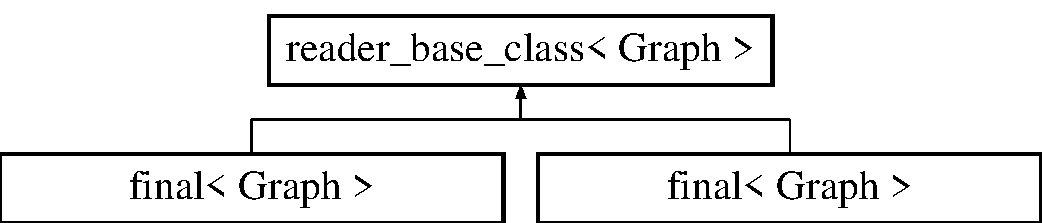
\includegraphics[height=2cm]{classreader__base__class}
\end{center}
\end{figure}
\subsection*{Public Types}
\begin{DoxyCompactItemize}
\item 
\hypertarget{classreader__base__class_add6b9a1702836a61d46c8484c34bc93a}{
typedef boost::graph\_\-traits$<$ Graph $>$::vertex\_\-descriptor {\bfseries Vertex\_\-desc}}
\label{classreader__base__class_add6b9a1702836a61d46c8484c34bc93a}

\item 
\hypertarget{classreader__base__class_a4f5b7d229edcf52020b99bacb402e7ba}{
typedef boost::graph\_\-traits$<$ Graph $>$::edge\_\-descriptor {\bfseries Edge\_\-desc}}
\label{classreader__base__class_a4f5b7d229edcf52020b99bacb402e7ba}

\end{DoxyCompactItemize}
\subsection*{Public Member Functions}
\begin{DoxyCompactItemize}
\item 
\hypertarget{classreader__base__class_a43fc72713a7023fce7eaa15266b6fb6f}{
\hyperlink{classreader__base__class_a43fc72713a7023fce7eaa15266b6fb6f}{reader\_\-base\_\-class} (Graph \&\_\-G)}
\label{classreader__base__class_a43fc72713a7023fce7eaa15266b6fb6f}

\begin{DoxyCompactList}\small\item\em Default constructor (we need however to initialize the reference). \item\end{DoxyCompactList}\item 
\hypertarget{classreader__base__class_aa24f5907deb19cfc75480de9f6535fe2}{
\hyperlink{classreader__base__class_aa24f5907deb19cfc75480de9f6535fe2}{reader\_\-base\_\-class} (Graph \&\_\-G, std::string \_\-file\_\-name, unsigned int \_\-num\_\-dummy\_\-lines)}
\label{classreader__base__class_aa24f5907deb19cfc75480de9f6535fe2}

\begin{DoxyCompactList}\small\item\em Constructor: assign only num\_\-dummy\_\-lines, empty graph. \item\end{DoxyCompactList}\item 
\hypertarget{classreader__base__class_a37c8eda56c3b51c2e5aa1b09fc689503}{
\hyperlink{classreader__base__class_a37c8eda56c3b51c2e5aa1b09fc689503}{reader\_\-base\_\-class} (\hyperlink{classreader__base__class}{reader\_\-base\_\-class} const \&)}
\label{classreader__base__class_a37c8eda56c3b51c2e5aa1b09fc689503}

\begin{DoxyCompactList}\small\item\em Default copy constructor. \item\end{DoxyCompactList}\item 
\hypertarget{classreader__base__class_a7629888633c2f453b792d2e63adad1d8}{
\hyperlink{classreader__base__class}{reader\_\-base\_\-class} \& \hyperlink{classreader__base__class_a7629888633c2f453b792d2e63adad1d8}{operator=} (\hyperlink{classreader__base__class}{reader\_\-base\_\-class} const \&)}
\label{classreader__base__class_a7629888633c2f453b792d2e63adad1d8}

\begin{DoxyCompactList}\small\item\em Assignement operator. \item\end{DoxyCompactList}\item 
\hypertarget{classreader__base__class_a001ba0a21c6099f0fc58acabe8852491}{
virtual \hyperlink{classreader__base__class_a001ba0a21c6099f0fc58acabe8852491}{$\sim$reader\_\-base\_\-class} ()}
\label{classreader__base__class_a001ba0a21c6099f0fc58acabe8852491}

\begin{DoxyCompactList}\small\item\em Destructor (needed?). \item\end{DoxyCompactList}\item 
\hypertarget{classreader__base__class_a5020c9b926b79bf1d9958215498d9e50}{
virtual void \hyperlink{classreader__base__class_a5020c9b926b79bf1d9958215498d9e50}{set\_\-input\_\-file} (std::string \_\-file\_\-name)}
\label{classreader__base__class_a5020c9b926b79bf1d9958215498d9e50}

\begin{DoxyCompactList}\small\item\em It allows to set the input file. \item\end{DoxyCompactList}\item 
\hypertarget{classreader__base__class_ac30077974d31badd9205f39f928e085f}{
virtual void \hyperlink{classreader__base__class_ac30077974d31badd9205f39f928e085f}{set\_\-num\_\-dummy\_\-lines} (unsigned int const \&\_\-num\_\-dummy\_\-lines)}
\label{classreader__base__class_ac30077974d31badd9205f39f928e085f}

\begin{DoxyCompactList}\small\item\em It allows to set both num\_\-dummy\_\-lines and current\_\-line\_\-number (they must have the same value). \item\end{DoxyCompactList}\item 
\hypertarget{classreader__base__class_ac6d07ef07127e4b172ccfac4e7aabda3}{
virtual void \hyperlink{classreader__base__class_ac6d07ef07127e4b172ccfac4e7aabda3}{read\_\-input\_\-file} ()}
\label{classreader__base__class_ac6d07ef07127e4b172ccfac4e7aabda3}

\begin{DoxyCompactList}\small\item\em Read the input file. \item\end{DoxyCompactList}\item 
\hypertarget{classreader__base__class_aced9ab4a76f00617de238ded83d4f873}{
virtual void \hyperlink{classreader__base__class_aced9ab4a76f00617de238ded83d4f873}{ignore\_\-dummy\_\-lines} (std::ifstream \&file)}
\label{classreader__base__class_aced9ab4a76f00617de238ded83d4f873}

\begin{DoxyCompactList}\small\item\em It ignores the first n lines, that are headers, in the input file. \item\end{DoxyCompactList}\item 
\hypertarget{classreader__base__class_a87b9c0f6d6100bab6c8d8ccf0c3a1e7e}{
virtual void \hyperlink{classreader__base__class_a87b9c0f6d6100bab6c8d8ccf0c3a1e7e}{read\_\-data\_\-from\_\-line} (std::istringstream \&temp)=0}
\label{classreader__base__class_a87b9c0f6d6100bab6c8d8ccf0c3a1e7e}

\begin{DoxyCompactList}\small\item\em It describes how to read each line in the input file, and in which variables to store the data. \item\end{DoxyCompactList}\item 
\hypertarget{classreader__base__class_a536131b6cc6f007b87735626c29650c6}{
virtual void \hyperlink{classreader__base__class_a536131b6cc6f007b87735626c29650c6}{build\_\-graph} ()=0}
\label{classreader__base__class_a536131b6cc6f007b87735626c29650c6}

\begin{DoxyCompactList}\small\item\em It build the graph one edge at a time, called many times from an external loop. \item\end{DoxyCompactList}\item 
\hypertarget{classreader__base__class_af9dd018f3818e2ec25ab4de7ab1d1275}{
virtual void \hyperlink{classreader__base__class_af9dd018f3818e2ec25ab4de7ab1d1275}{give\_\-new\_\-source\_\-properties} ()=0}
\label{classreader__base__class_af9dd018f3818e2ec25ab4de7ab1d1275}

\begin{DoxyCompactList}\small\item\em It assigns properties to new\_\-source in the rigth way. It has to be called in \hyperlink{classreader__base__class_a536131b6cc6f007b87735626c29650c6}{build\_\-graph()}! \item\end{DoxyCompactList}\item 
\hypertarget{classreader__base__class_ab98ff4a8a406effb25f0bc4ce89ae3df}{
virtual void \hyperlink{classreader__base__class_ab98ff4a8a406effb25f0bc4ce89ae3df}{give\_\-new\_\-target\_\-properties} ()=0}
\label{classreader__base__class_ab98ff4a8a406effb25f0bc4ce89ae3df}

\begin{DoxyCompactList}\small\item\em It assigns properties to new\_\-target in the right way. It has to be called in \hyperlink{classreader__base__class_a536131b6cc6f007b87735626c29650c6}{build\_\-graph()}! \item\end{DoxyCompactList}\item 
\hypertarget{classreader__base__class_add3be7869df5b87ba40080897a5d9f1a}{
virtual void \hyperlink{classreader__base__class_add3be7869df5b87ba40080897a5d9f1a}{give\_\-new\_\-edge\_\-properties} ()=0}
\label{classreader__base__class_add3be7869df5b87ba40080897a5d9f1a}

\begin{DoxyCompactList}\small\item\em It assigns properties to new\_\-edge in the rigth way. It has to be called in \hyperlink{classreader__base__class_a536131b6cc6f007b87735626c29650c6}{build\_\-graph()}! \item\end{DoxyCompactList}\item 
\hypertarget{classreader__base__class_a7cdc6fe09127ebba4a91dcbec6e774c2}{
virtual void \hyperlink{classreader__base__class_a7cdc6fe09127ebba4a91dcbec6e774c2}{if\_\-edge\_\-not\_\-inserted} ()}
\label{classreader__base__class_a7cdc6fe09127ebba4a91dcbec6e774c2}

\begin{DoxyCompactList}\small\item\em It deals with wrong insertion of an edge.  It can be called only after a call to boost::add\_\-edge with the pair $<$Edge\_\-desc, bool$>$ as return value. In this way the value of edge\_\-inserted is set up. \item\end{DoxyCompactList}\end{DoxyCompactItemize}
\subsection*{Protected Attributes}
\begin{DoxyCompactItemize}
\item 
\hypertarget{classreader__base__class_a8453e0babb48c829551ed86a076990a0}{
Graph \& \hyperlink{classreader__base__class_a8453e0babb48c829551ed86a076990a0}{G}}
\label{classreader__base__class_a8453e0babb48c829551ed86a076990a0}

\begin{DoxyCompactList}\small\item\em A reference is used to represent the Graph.  Using a reference allows us not to copy the whole graph outside the class once finished to read data and to build the graph. In this way we build the pre-\/existent graph (created in the main) while reading the input file. We do not use extra memory. \item\end{DoxyCompactList}\item 
\hypertarget{classreader__base__class_ace1598042648e8af4275063a53bb2dc9}{
std::string \hyperlink{classreader__base__class_ace1598042648e8af4275063a53bb2dc9}{file\_\-name}}
\label{classreader__base__class_ace1598042648e8af4275063a53bb2dc9}

\begin{DoxyCompactList}\small\item\em The string in which is stored the name of the input file to read. \item\end{DoxyCompactList}\item 
\hypertarget{classreader__base__class_a68001946415ed68d9bd2b8e5fd01cbc3}{
unsigned int \hyperlink{classreader__base__class_a68001946415ed68d9bd2b8e5fd01cbc3}{num\_\-dummy\_\-lines}}
\label{classreader__base__class_a68001946415ed68d9bd2b8e5fd01cbc3}

\begin{DoxyCompactList}\small\item\em The numbers of initial lines (headers) that the reader has to skip to read useful data. \item\end{DoxyCompactList}\item 
\hypertarget{classreader__base__class_adf0049e509e246a1de1a9076255ab69a}{
std::string \hyperlink{classreader__base__class_adf0049e509e246a1de1a9076255ab69a}{line}}
\label{classreader__base__class_adf0049e509e246a1de1a9076255ab69a}

\begin{DoxyCompactList}\small\item\em This will contain one line of the input file, to parse. \item\end{DoxyCompactList}\item 
\hypertarget{classreader__base__class_a22708fe953f4e0221270f28f309f80f4}{
Vertex\_\-desc \hyperlink{classreader__base__class_a22708fe953f4e0221270f28f309f80f4}{new\_\-source}}
\label{classreader__base__class_a22708fe953f4e0221270f28f309f80f4}

\begin{DoxyCompactList}\small\item\em The vertex descriptor for the source of the new edge added. \item\end{DoxyCompactList}\item 
\hypertarget{classreader__base__class_a3215bc334e6f5e7ca1601529150e4ce7}{
Vertex\_\-desc \hyperlink{classreader__base__class_a3215bc334e6f5e7ca1601529150e4ce7}{new\_\-target}}
\label{classreader__base__class_a3215bc334e6f5e7ca1601529150e4ce7}

\begin{DoxyCompactList}\small\item\em The vertex descriptor for the target of the new edge added. \item\end{DoxyCompactList}\item 
\hypertarget{classreader__base__class_ab002060e56625ce5d422e811015ae90e}{
Edge\_\-desc \hyperlink{classreader__base__class_ab002060e56625ce5d422e811015ae90e}{new\_\-edge}}
\label{classreader__base__class_ab002060e56625ce5d422e811015ae90e}

\begin{DoxyCompactList}\small\item\em The edge descriptor for the new edge. \item\end{DoxyCompactList}\item 
\hypertarget{classreader__base__class_a59220f3fd7d9ed4effa57d0175f1d420}{
bool \hyperlink{classreader__base__class_a59220f3fd7d9ed4effa57d0175f1d420}{edge\_\-inserted}}
\label{classreader__base__class_a59220f3fd7d9ed4effa57d0175f1d420}

\begin{DoxyCompactList}\small\item\em Bool returned in a pair with an edge descriptor by add\_\-edge function.  The value is assigned when trying to insert an edge in the graph. It is set to true if the edge was succesfully inserted, false otherwise. \item\end{DoxyCompactList}\item 
\hypertarget{classreader__base__class_ab2b9bc60ece613cb7de32b02dae65f15}{
unsigned int \hyperlink{classreader__base__class_ab2b9bc60ece613cb7de32b02dae65f15}{current\_\-line\_\-number}}
\label{classreader__base__class_ab2b9bc60ece613cb7de32b02dae65f15}

\begin{DoxyCompactList}\small\item\em It tracks the current line of the input file. \item\end{DoxyCompactList}\end{DoxyCompactItemize}
\subsubsection*{template$<$typename Graph$>$ class reader\_\-base\_\-class$<$ Graph $>$}



The documentation for this class was generated from the following file:\begin{DoxyCompactItemize}
\item 
include/\hyperlink{reader__base__class_8hpp}{reader\_\-base\_\-class.hpp}\end{DoxyCompactItemize}

\hypertarget{structvertex__data__structure}{
\section{vertex\_\-data\_\-structure$<$ dim $>$ Struct Template Reference}
\label{structvertex__data__structure}\index{vertex\_\-data\_\-structure@{vertex\_\-data\_\-structure}}
}
\subsection*{Public Attributes}
\begin{DoxyCompactItemize}
\item 
\hypertarget{structvertex__data__structure_a974f87b132b5a0948ccf069170d3a4ba}{
unsigned int {\bfseries vertex\_\-id} = 0}
\label{structvertex__data__structure_a974f87b132b5a0948ccf069170d3a4ba}

\item 
\hypertarget{structvertex__data__structure_a48c25a9d4e52b5a2cdec83d9633a0c5c}{
std::string {\bfseries label} = \char`\"{}\char`\"{}}
\label{structvertex__data__structure_a48c25a9d4e52b5a2cdec83d9633a0c5c}

\item 
\hypertarget{structvertex__data__structure_a620eae50faa20408863c22e01689387e}{
point$<$ dim $>$ {\bfseries coord}}
\label{structvertex__data__structure_a620eae50faa20408863c22e01689387e}

\end{DoxyCompactItemize}
\subsubsection*{template$<$unsigned int dim$>$ struct vertex\_\-data\_\-structure$<$ dim $>$}



The documentation for this struct was generated from the following file:\begin{DoxyCompactItemize}
\item 
include/\hyperlink{data__structure_8hpp}{data\_\-structure.hpp}\end{DoxyCompactItemize}

\hypertarget{structZunino__edge__data}{
\section{Zunino\_\-edge\_\-data Struct Reference}
\label{structZunino__edge__data}\index{Zunino\_\-edge\_\-data@{Zunino\_\-edge\_\-data}}
}
\subsection*{Public Attributes}
\begin{DoxyCompactItemize}
\item 
\hypertarget{structZunino__edge__data_a73441af93ae1f5b358840404cfa6e0e3}{
double {\bfseries capacity}}
\label{structZunino__edge__data_a73441af93ae1f5b358840404cfa6e0e3}

\item 
\hypertarget{structZunino__edge__data_af9a655836071f05edf61648d3d2c5258}{
double {\bfseries length}}
\label{structZunino__edge__data_af9a655836071f05edf61648d3d2c5258}

\end{DoxyCompactItemize}


The documentation for this struct was generated from the following file:\begin{DoxyCompactItemize}
\item 
include/\hyperlink{new__reader__Zunino_8hpp}{new\_\-reader\_\-Zunino.hpp}\end{DoxyCompactItemize}

\hypertarget{structZunino__edge__property__t}{
\section{Zunino\_\-edge\_\-property\_\-t Struct Reference}
\label{structZunino__edge__property__t}\index{Zunino\_\-edge\_\-property\_\-t@{Zunino\_\-edge\_\-property\_\-t}}
}
\subsection*{Public Attributes}
\begin{DoxyCompactItemize}
\item 
\hypertarget{structZunino__edge__property__t_adb224930eb2b0572fc47f01e96ce0d3f}{
double {\bfseries capacity}}
\label{structZunino__edge__property__t_adb224930eb2b0572fc47f01e96ce0d3f}

\item 
\hypertarget{structZunino__edge__property__t_a8277c98a24dd9a88a7947154b89c9b86}{
double {\bfseries length}}
\label{structZunino__edge__property__t_a8277c98a24dd9a88a7947154b89c9b86}

\end{DoxyCompactItemize}


The documentation for this struct was generated from the following file:\begin{DoxyCompactItemize}
\item 
include/\hyperlink{Zunino__edge__property_8hpp}{Zunino\_\-edge\_\-property.hpp}\end{DoxyCompactItemize}

\hypertarget{classZunino__reader}{
\section{Zunino\_\-reader$<$ Zunino\_\-source\_\-data, Zunino\_\-target\_\-data, Zunino\_\-edge\_\-data, Zunino\_\-topological\_\-data $>$ Class Template Reference}
\label{classZunino__reader}\index{Zunino\_\-reader@{Zunino\_\-reader}}
}
Inheritance diagram for Zunino\_\-reader$<$ Zunino\_\-source\_\-data, Zunino\_\-target\_\-data, Zunino\_\-edge\_\-data, Zunino\_\-topological\_\-data $>$::\begin{figure}[H]
\begin{center}
\leavevmode
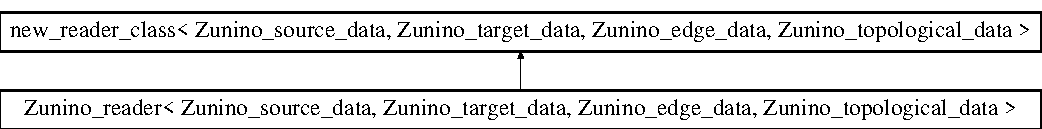
\includegraphics[height=1.73107cm]{classZunino__reader}
\end{center}
\end{figure}
\subsection*{Public Member Functions}
\begin{DoxyCompactItemize}
\item 
\hypertarget{classZunino__reader_a0d7f1b5865e3c9e4ea0d95b231781963}{
virtual void \hyperlink{classZunino__reader_a0d7f1b5865e3c9e4ea0d95b231781963}{get\_\-data\_\-from\_\-line} ()}
\label{classZunino__reader_a0d7f1b5865e3c9e4ea0d95b231781963}

\begin{DoxyCompactList}\small\item\em Reads the data from one single line. It has to be specified by the user  It reads data form the istringstream iss\_\-line that is defined as an attribute of the class and it is updated after every call of \hyperlink{classnew__reader__class_a95f6bf521a51258b14e5b5755fe5e75f}{read\_\-line()}. \item\end{DoxyCompactList}\item 
\hypertarget{classZunino__reader_a09df2a15d819e203badb5fea1fa37d48}{
virtual \hyperlink{structZunino__source__data}{Zunino\_\-source\_\-data} \hyperlink{classZunino__reader_a09df2a15d819e203badb5fea1fa37d48}{get\_\-source\_\-data} ()}
\label{classZunino__reader_a09df2a15d819e203badb5fea1fa37d48}

\begin{DoxyCompactList}\small\item\em A method to get the right data to append to the source. \item\end{DoxyCompactList}\item 
\hypertarget{classZunino__reader_a5c22d440991382506b268d2051a52826}{
virtual \hyperlink{structZunino__target__data}{Zunino\_\-target\_\-data} \hyperlink{classZunino__reader_a5c22d440991382506b268d2051a52826}{get\_\-target\_\-data} ()}
\label{classZunino__reader_a5c22d440991382506b268d2051a52826}

\begin{DoxyCompactList}\small\item\em A method to get the right data to append to the target. \item\end{DoxyCompactList}\item 
\hypertarget{classZunino__reader_a1b5acdd2df1785085d30e2a9da093afa}{
virtual \hyperlink{structZunino__edge__data}{Zunino\_\-edge\_\-data} \hyperlink{classZunino__reader_a1b5acdd2df1785085d30e2a9da093afa}{get\_\-edge\_\-data} ()}
\label{classZunino__reader_a1b5acdd2df1785085d30e2a9da093afa}

\begin{DoxyCompactList}\small\item\em A method to get the right data to append to an edge. \item\end{DoxyCompactList}\item 
\hypertarget{classZunino__reader_a0c19b2f15fe48f52fc28a89717b93ab4}{
virtual \hyperlink{structZunino__topological__data}{Zunino\_\-topological\_\-data} {\bfseries get\_\-topologica\_\-data} ()}
\label{classZunino__reader_a0c19b2f15fe48f52fc28a89717b93ab4}

\end{DoxyCompactItemize}
\subsubsection*{template$<$typename Zunino\_\-source\_\-data, typename Zunino\_\-target\_\-data, typename Zunino\_\-edge\_\-data, typename Zunino\_\-topological\_\-data$>$ class Zunino\_\-reader$<$ Zunino\_\-source\_\-data, Zunino\_\-target\_\-data, Zunino\_\-edge\_\-data, Zunino\_\-topological\_\-data $>$}



The documentation for this class was generated from the following file:\begin{DoxyCompactItemize}
\item 
include/\hyperlink{new__reader__Zunino_8hpp}{new\_\-reader\_\-Zunino.hpp}\end{DoxyCompactItemize}

\hypertarget{structZunino__source__data}{
\section{Zunino\_\-source\_\-data Struct Reference}
\label{structZunino__source__data}\index{Zunino\_\-source\_\-data@{Zunino\_\-source\_\-data}}
}
\subsection*{Public Attributes}
\begin{DoxyCompactItemize}
\item 
\hypertarget{structZunino__source__data_a6dfd3bca7be19875015816dde7d6228f}{
\hyperlink{classBGLgeom_1_1point}{BGLgeom::point}$<$ 3 $>$ {\bfseries SRC}}
\label{structZunino__source__data_a6dfd3bca7be19875015816dde7d6228f}

\end{DoxyCompactItemize}


The documentation for this struct was generated from the following file:\begin{DoxyCompactItemize}
\item 
include/\hyperlink{new__reader__Zunino_8hpp}{new\_\-reader\_\-Zunino.hpp}\end{DoxyCompactItemize}

\hypertarget{structZunino__target__data}{
\section{Zunino\_\-target\_\-data Struct Reference}
\label{structZunino__target__data}\index{Zunino\_\-target\_\-data@{Zunino\_\-target\_\-data}}
}
\subsection*{Public Attributes}
\begin{DoxyCompactItemize}
\item 
\hypertarget{structZunino__target__data_a4c43a30f956f9cd43b94a84b856819ac}{
\hyperlink{classBGLgeom_1_1point}{BGLgeom::point}$<$ 3 $>$ {\bfseries TGT}}
\label{structZunino__target__data_a4c43a30f956f9cd43b94a84b856819ac}

\end{DoxyCompactItemize}


The documentation for this struct was generated from the following file:\begin{DoxyCompactItemize}
\item 
include/\hyperlink{new__reader__Zunino_8hpp}{new\_\-reader\_\-Zunino.hpp}\end{DoxyCompactItemize}

\hypertarget{structZunino__topological__data}{
\section{Zunino\_\-topological\_\-data Struct Reference}
\label{structZunino__topological__data}\index{Zunino\_\-topological\_\-data@{Zunino\_\-topological\_\-data}}
}
\subsection*{Public Attributes}
\begin{DoxyCompactItemize}
\item 
\hypertarget{structZunino__topological__data_a4775b816ecc3ccd5b21dd48e972831e2}{
unsigned int {\bfseries src}}
\label{structZunino__topological__data_a4775b816ecc3ccd5b21dd48e972831e2}

\item 
\hypertarget{structZunino__topological__data_a80b7569157acbcef935a6aa0b6191171}{
unsigned int {\bfseries tgt}}
\label{structZunino__topological__data_a80b7569157acbcef935a6aa0b6191171}

\end{DoxyCompactItemize}


The documentation for this struct was generated from the following file:\begin{DoxyCompactItemize}
\item 
include/\hyperlink{new__reader__Zunino_8hpp}{new\_\-reader\_\-Zunino.hpp}\end{DoxyCompactItemize}

\chapter{File Documentation}
\hypertarget{compute__euclidean__distance_8hpp}{
\section{include/compute\_\-euclidean\_\-distance.hpp File Reference}
\label{compute__euclidean__distance_8hpp}\index{include/compute\_\-euclidean\_\-distance.hpp@{include/compute\_\-euclidean\_\-distance.hpp}}
}


Computes the euclidean distance between two given vertices.  
{\ttfamily \#include \char`\"{}compute\_\-euclidean\_\-distance\_\-imp.hpp\char`\"{}}\par
\subsection*{Functions}
\begin{DoxyCompactItemize}
\item 
\hypertarget{compute__euclidean__distance_8hpp_adf0c8ac9a0cab841c1534f9f5411a1c3}{
{\footnotesize template$<$typename Graph $>$ }\\double {\bfseries compute\_\-euclidean\_\-distance} (typename boost::graph\_\-traits$<$ Graph $>$::vertex\_\-descriptor a, typename boost::graph\_\-traits$<$ Graph $>$::vertex\_\-descriptor b, Graph const \&G)}
\label{compute__euclidean__distance_8hpp_adf0c8ac9a0cab841c1534f9f5411a1c3}

\end{DoxyCompactItemize}


\subsection{Detailed Description}
Computes the euclidean distance between two given vertices. \begin{DoxyAuthor}{Author}
Ilaria Speranza \& Mattia Tantardini 
\end{DoxyAuthor}
\begin{DoxyDate}{Date}
Sep 2016. 
\end{DoxyDate}

\hypertarget{data__structure_8hpp}{
\section{include/data\_\-structure.hpp File Reference}
\label{data__structure_8hpp}\index{include/data\_\-structure.hpp@{include/data\_\-structure.hpp}}
}


Declaration of generic data structure to represent vertex and edge properties.  
{\ttfamily \#include \char`\"{}user\_\-data\_\-structure.hpp\char`\"{}}\par
{\ttfamily \#include $<$string$>$}\par
{\ttfamily \#include \char`\"{}generic\_\-edge\_\-geometry.hpp\char`\"{}}\par
{\ttfamily \#include \char`\"{}generic\_\-point.hpp\char`\"{}}\par
\subsection*{Classes}
\begin{DoxyCompactItemize}
\item 
class \hyperlink{structdata__structure}{data\_\-structure$<$ Edge\_\-data\_\-structure, Vertex\_\-data\_\-structure $>$}
\begin{DoxyCompactList}\small\item\em An abstract class to handle the user definition data structure  The users has to specify, in the derived class, all variables he need in order to store information read from the input file. Then, through the definition of Edge\_\-data\_\-structure and Vertex\_\-data\_\-structure, he can get separately all the information to put on edges and vertices. \item\end{DoxyCompactList}\item 
struct \hyperlink{structmy__edge}{my\_\-edge}
\item 
struct \hyperlink{structedge__data__structure}{edge\_\-data\_\-structure$<$ dim $>$}
\item 
struct \hyperlink{structvertex__data__structure}{vertex\_\-data\_\-structure$<$ dim $>$}
\item 
class \hyperlink{structdata__structure}{data\_\-structure$<$ Edge\_\-data\_\-structure, Vertex\_\-data\_\-structure $>$}
\begin{DoxyCompactList}\small\item\em An abstract class to handle the user definition data structure  The users has to specify, in the derived class, all variables he need in order to store information read from the input file. Then, through the definition of Edge\_\-data\_\-structure and Vertex\_\-data\_\-structure, he can get separately all the information to put on edges and vertices. \item\end{DoxyCompactList}\end{DoxyCompactItemize}
\subsection*{Functions}
\begin{DoxyCompactItemize}
\item 
\hypertarget{data__structure_8hpp_a07f7ad9a2dd195a85015db7be6b19777}{
{\bfseries get\_\-data\_\-from\_\-line} (std::ifstream \&in, \hyperlink{structdata__structure}{data\_\-structure} \&D)}
\label{data__structure_8hpp_a07f7ad9a2dd195a85015db7be6b19777}

\item 
\hypertarget{data__structure_8hpp_a227e3176fb34375a1d6f20a7723503f4}{
virtual read\_\-file \hyperlink{structmy__edge}{my\_\-edge} {\bfseries get\_\-edge\_\-data} ()}
\label{data__structure_8hpp_a227e3176fb34375a1d6f20a7723503f4}

\end{DoxyCompactItemize}
\subsection*{Variables}
\begin{DoxyCompactItemize}
\item 
\hypertarget{data__structure_8hpp_a6bb17dfa9d209fa07ee291676a748b7f}{
struct \hyperlink{structmy__edge}{my\_\-edge} {\bfseries length}}
\label{data__structure_8hpp_a6bb17dfa9d209fa07ee291676a748b7f}

\item 
\hypertarget{data__structure_8hpp_a16be187ac405f3bb61930a342b444253}{
point {\bfseries coord}}
\label{data__structure_8hpp_a16be187ac405f3bb61930a342b444253}

\end{DoxyCompactItemize}


\subsection{Detailed Description}
Declaration of generic data structure to represent vertex and edge properties. \begin{DoxyAuthor}{Author}
Ilaria Speranza \& Mattia Tantardini 
\end{DoxyAuthor}
\begin{DoxyDate}{Date}
Sept, 2016 
\end{DoxyDate}

\hypertarget{dijkstra_8hpp}{
\section{include/dijkstra.hpp File Reference}
\label{dijkstra_8hpp}\index{include/dijkstra.hpp@{include/dijkstra.hpp}}
}


Solves the single-\/source shortest-\/paths problem on a weighted, directed graph with non-\/negative edge weights.  This function takes in input the graph, the source vertex and two vectors, one for the distance map and the other for the predecessor map, which will be filled with the results of the algorithm.  
{\ttfamily \#include \char`\"{}boost/graph/dijkstra\_\-shortest\_\-paths.hpp\char`\"{}}\par
{\ttfamily \#include \char`\"{}Zunino\_\-edge\_\-property.hpp\char`\"{}}\par
{\ttfamily \#include \char`\"{}dijkstra\_\-imp.hpp\char`\"{}}\par
\subsection*{Functions}
\begin{DoxyCompactItemize}
\item 
\hypertarget{dijkstra_8hpp_ae594702e347d7f4cf72ff2ddf853f0af}{
{\footnotesize template$<$typename Graph $>$ }\\void {\bfseries dijkstra} (Graph const \&G, typename boost::graph\_\-traits$<$ Graph $>$::vertex\_\-descriptor const \&v, std::vector$<$ int $>$ \&distances, std::vector$<$ typename boost::graph\_\-traits$<$ Graph $>$::vertex\_\-descriptor $>$ \&predecessors)}
\label{dijkstra_8hpp_ae594702e347d7f4cf72ff2ddf853f0af}

\end{DoxyCompactItemize}


\subsection{Detailed Description}
Solves the single-\/source shortest-\/paths problem on a weighted, directed graph with non-\/negative edge weights.  This function takes in input the graph, the source vertex and two vectors, one for the distance map and the other for the predecessor map, which will be filled with the results of the algorithm. \begin{DoxyAuthor}{Author}
Ilaria Speranza \& Mattia Tantardini 
\end{DoxyAuthor}
\begin{DoxyDate}{Date}
Oct 2016. 
\end{DoxyDate}

\hypertarget{dijkstra__imp_8hpp}{
\section{include/dijkstra\_\-imp.hpp File Reference}
\label{dijkstra__imp_8hpp}\index{include/dijkstra\_\-imp.hpp@{include/dijkstra\_\-imp.hpp}}
}


Solves the single-\/source shortest-\/paths problem on a weighted, directed graph with non-\/negative edge weights. .  
\subsection*{Functions}
\begin{DoxyCompactItemize}
\item 
\hypertarget{dijkstra__imp_8hpp_ae594702e347d7f4cf72ff2ddf853f0af}{
{\footnotesize template$<$typename Graph $>$ }\\void {\bfseries dijkstra} (Graph const \&G, typename boost::graph\_\-traits$<$ Graph $>$::vertex\_\-descriptor const \&v, std::vector$<$ int $>$ \&distances, std::vector$<$ typename boost::graph\_\-traits$<$ Graph $>$::vertex\_\-descriptor $>$ \&predecessors)}
\label{dijkstra__imp_8hpp_ae594702e347d7f4cf72ff2ddf853f0af}

\end{DoxyCompactItemize}


\subsection{Detailed Description}
Solves the single-\/source shortest-\/paths problem on a weighted, directed graph with non-\/negative edge weights. . \begin{DoxyAuthor}{Author}
Ilaria Speranza \& Mattia Tantardini 
\end{DoxyAuthor}
\begin{DoxyDate}{Date}
Oct 2016. 
\end{DoxyDate}

\hypertarget{disjoint__components_8hpp}{
\section{include/disjoint\_\-components.hpp File Reference}
\label{disjoint__components_8hpp}\index{include/disjoint\_\-components.hpp@{include/disjoint\_\-components.hpp}}
}


Identifies if there are fully disconnected subgraphs.. .  
{\ttfamily \#include $<$map$>$}\par
{\ttfamily \#include $<$tuple$>$}\par
{\ttfamily \#include $<$iostream$>$}\par
{\ttfamily \#include $<$boost/graph/graph\_\-traits.hpp$>$}\par
{\ttfamily \#include \char`\"{}our\_\-disjoint\_\-sets.hpp\char`\"{}}\par
{\ttfamily \#include \char`\"{}disjoint\_\-components\_\-imp.hpp\char`\"{}}\par
\subsection*{Functions}
\begin{DoxyCompactItemize}
\item 
{\footnotesize template$<$typename Graph $>$ }\\void \hyperlink{disjoint__components_8hpp_a098a633d00c11d9e718e8aae256351fa}{disjoint\_\-components} (Graph \&G)
\end{DoxyCompactItemize}


\subsection{Detailed Description}
Identifies if there are fully disconnected subgraphs.. . \begin{DoxyAuthor}{Author}
Ilaria Speranza \& Mattia Tantardini 
\end{DoxyAuthor}
\begin{DoxyDate}{Date}
Sep 2016. 
\end{DoxyDate}


\subsection{Function Documentation}
\hypertarget{disjoint__components_8hpp_a098a633d00c11d9e718e8aae256351fa}{
\index{disjoint\_\-components.hpp@{disjoint\_\-components.hpp}!disjoint\_\-components@{disjoint\_\-components}}
\index{disjoint\_\-components@{disjoint\_\-components}!disjoint_components.hpp@{disjoint\_\-components.hpp}}
\subsubsection[{disjoint\_\-components}]{\setlength{\rightskip}{0pt plus 5cm}template$<$typename Graph $>$ void disjoint\_\-components (Graph \& {\em G})\hspace{0.3cm}{\ttfamily  \mbox{[}inline\mbox{]}}}}
\label{disjoint__components_8hpp_a098a633d00c11d9e718e8aae256351fa}
Given a graph, this function checks whether there are fully disconnected subgraphs, i.e. subgraphs with no edge connecting each other. It returns a map which associates each vertex with an integer identifying the subgraph it belongs to. 
\hypertarget{disjoint__components__imp_8hpp}{
\section{include/disjoint\_\-components\_\-imp.hpp File Reference}
\label{disjoint__components__imp_8hpp}\index{include/disjoint\_\-components\_\-imp.hpp@{include/disjoint\_\-components\_\-imp.hpp}}
}


Identifies if there are fully disconnected subgraphs.  
\subsection*{Functions}
\begin{DoxyCompactItemize}
\item 
{\footnotesize template$<$typename Graph $>$ }\\void \hyperlink{disjoint__components__imp_8hpp_a098a633d00c11d9e718e8aae256351fa}{disjoint\_\-components} (Graph \&G)
\end{DoxyCompactItemize}


\subsection{Detailed Description}
Identifies if there are fully disconnected subgraphs. \begin{DoxyAuthor}{Author}
Ilaria Speranza \& Mattia Tantardini 
\end{DoxyAuthor}
\begin{DoxyDate}{Date}
Sep 2016.  Note: the algorithm is not very well. It can be bettered, in particular when changing all the labels of a big component that we have to move in another small component. Better to move the smaller into the bigger. 
\end{DoxyDate}


\subsection{Function Documentation}
\hypertarget{disjoint__components__imp_8hpp_a098a633d00c11d9e718e8aae256351fa}{
\index{disjoint\_\-components\_\-imp.hpp@{disjoint\_\-components\_\-imp.hpp}!disjoint\_\-components@{disjoint\_\-components}}
\index{disjoint\_\-components@{disjoint\_\-components}!disjoint_components_imp.hpp@{disjoint\_\-components\_\-imp.hpp}}
\subsubsection[{disjoint\_\-components}]{\setlength{\rightskip}{0pt plus 5cm}template$<$typename Graph $>$ void disjoint\_\-components (Graph \& {\em G})\hspace{0.3cm}{\ttfamily  \mbox{[}inline\mbox{]}}}}
\label{disjoint__components__imp_8hpp_a098a633d00c11d9e718e8aae256351fa}
Given a graph, this function checks whether there are fully disconnected subgraphs, i.e. subgraphs with no edge connecting each other. It returns a map which associates each vertex with an integer identifying the subgraph it belongs to. 
\hypertarget{edge__geometry_8hpp}{
\section{include/edge\_\-geometry.hpp File Reference}
\label{edge__geometry_8hpp}\index{include/edge\_\-geometry.hpp@{include/edge\_\-geometry.hpp}}
}


Virtual base class for the geometry of an edge .  
\subsection*{Classes}
\begin{DoxyCompactItemize}
\item 
class \hyperlink{classBGLgeom_1_1edge__geometry}{BGLgeom::edge\_\-geometry$<$ dim $>$}
\end{DoxyCompactItemize}


\subsection{Detailed Description}
Virtual base class for the geometry of an edge . \begin{DoxyAuthor}{Author}
Ilaria Speranza \& Mattia Tantardini 
\end{DoxyAuthor}
\begin{DoxyDate}{Date}
Sept, 2016 
\end{DoxyDate}

\hypertarget{Forma__edge__property_8hpp}{
\section{include/Forma\_\-edge\_\-property.hpp File Reference}
\label{Forma__edge__property_8hpp}\index{include/Forma\_\-edge\_\-property.hpp@{include/Forma\_\-edge\_\-property.hpp}}
}


This contains the struct for edge properties that has to be used for Formaggia's example .  
\subsection*{Classes}
\begin{DoxyCompactItemize}
\item 
class \hyperlink{classedge__parametrization}{edge\_\-parametrization}
\begin{DoxyCompactList}\small\item\em This class holds the parametrization of the edge. \item\end{DoxyCompactList}\item 
struct \hyperlink{structForma__edge__property__t}{Forma\_\-edge\_\-property\_\-t}
\end{DoxyCompactItemize}


\subsection{Detailed Description}
This contains the struct for edge properties that has to be used for Formaggia's example . \begin{DoxyAuthor}{Author}
Ilaria Speranza \& Mattia Tantardini 
\end{DoxyAuthor}
\begin{DoxyDate}{Date}
Sept, 2016 
\end{DoxyDate}

\hypertarget{Forma__vertex__property_8hpp}{
\section{include/Forma\_\-vertex\_\-property.hpp File Reference}
\label{Forma__vertex__property_8hpp}\index{include/Forma\_\-vertex\_\-property.hpp@{include/Forma\_\-vertex\_\-property.hpp}}
}


This contains the struct for vertex properties that has to be used for Formaggia's example .  
{\ttfamily \#include \char`\"{}generic\_\-point.hpp\char`\"{}}\par
\subsection*{Classes}
\begin{DoxyCompactItemize}
\item 
struct \hyperlink{structForma__vertex__property__t}{Forma\_\-vertex\_\-property\_\-t}
\begin{DoxyCompactList}\small\item\em This struct contains the vertex property for Formaggia's example. \item\end{DoxyCompactList}\end{DoxyCompactItemize}


\subsection{Detailed Description}
This contains the struct for vertex properties that has to be used for Formaggia's example . \begin{DoxyAuthor}{Author}
Ilaria Speranza \& Mattia Tantardini 
\end{DoxyAuthor}
\begin{DoxyDate}{Date}
Sept, 2016 
\end{DoxyDate}

\hypertarget{generic__edge__geometry_8hpp}{
\section{include/generic\_\-edge\_\-geometry.hpp File Reference}
\label{generic__edge__geometry_8hpp}\index{include/generic\_\-edge\_\-geometry.hpp@{include/generic\_\-edge\_\-geometry.hpp}}
}


Class for circular geometry of an edge .  
{\ttfamily \#include $<$array$>$}\par
{\ttfamily \#include $<$functional$>$}\par
{\ttfamily \#include \char`\"{}generic\_\-point.hpp\char`\"{}}\par
{\ttfamily \#include \char`\"{}edge\_\-geometry.hpp\char`\"{}}\par
\subsection*{Classes}
\begin{DoxyCompactItemize}
\item 
class \hyperlink{classBGLgeom_1_1generic__edge__geometry}{BGLgeom::generic\_\-edge\_\-geometry$<$ dim $>$}
\end{DoxyCompactItemize}


\subsection{Detailed Description}
Class for circular geometry of an edge . class for the generic geometry of an edge 

\begin{DoxyAuthor}{Author}
Ilaria Speranza \& Mattia Tantardini 
\end{DoxyAuthor}
\begin{DoxyDate}{Date}
Sept, 2016 
\end{DoxyDate}

\hypertarget{generic__point_8hpp}{
\section{include/generic\_\-point.hpp File Reference}
\label{generic__point_8hpp}\index{include/generic\_\-point.hpp@{include/generic\_\-point.hpp}}
}


Templete class to handle points in 2D or 3D (or even greater).  
{\ttfamily \#include $<$array$>$}\par
{\ttfamily \#include $<$iostream$>$}\par
{\ttfamily \#include $<$initializer\_\-list$>$}\par
{\ttfamily \#include $<$type\_\-traits$>$}\par
\subsection*{Classes}
\begin{DoxyCompactItemize}
\item 
class \hyperlink{classBGLgeom_1_1point}{BGLgeom::point$<$ dim, Storage\_\-t $>$}
\begin{DoxyCompactList}\small\item\em Class template for storing the vertex coordinates in n-\/dimentional space. \item\end{DoxyCompactList}\end{DoxyCompactItemize}


\subsection{Detailed Description}
Templete class to handle points in 2D or 3D (or even greater). \begin{DoxyAuthor}{Author}
Ilaria Speranza and Mattia Tantardini 
\end{DoxyAuthor}
\begin{DoxyDate}{Date}
Sept, 2016 
\end{DoxyDate}

\hypertarget{graph__builder_8hpp}{
\section{include/graph\_\-builder.hpp File Reference}
\label{graph__builder_8hpp}\index{include/graph\_\-builder.hpp@{include/graph\_\-builder.hpp}}
}


Utilities to build a graph.  
{\ttfamily \#include $<$vector$>$}\par
{\ttfamily \#include $<$boost/graph/graph\_\-traits.hpp$>$}\par
{\ttfamily \#include \char`\"{}generic\_\-point.hpp\char`\"{}}\par
\subsection*{Functions}
\begin{DoxyCompactItemize}
\item 
\hypertarget{graph__builder_8hpp_a9ace6a37932f7a74fd2445b4dac6d0e5}{
{\footnotesize template$<$typename Graph , typename Source\_\-data\_\-structure $>$ }\\void \hyperlink{graph__builder_8hpp_a9ace6a37932f7a74fd2445b4dac6d0e5}{give\_\-source\_\-properties} (Source\_\-data\_\-structure const \&D, boost::graph\_\-traits$<$ Graph $>$::vertex\_\-descriptor const \&v, Graph \&G)}
\label{graph__builder_8hpp_a9ace6a37932f7a74fd2445b4dac6d0e5}

\begin{DoxyCompactList}\small\item\em Giving to source node v all properties through assigning the Source\_\-data\_\-structure. \item\end{DoxyCompactList}\item 
\hypertarget{graph__builder_8hpp_a8ded846b7c184caa0b3e7dd4c9ac57d9}{
{\footnotesize template$<$typename Graph , typename Target\_\-data\_\-structure $>$ }\\void \hyperlink{graph__builder_8hpp_a8ded846b7c184caa0b3e7dd4c9ac57d9}{give\_\-target\_\-properties} (Target\_\-data\_\-structure const \&D, boost::graph\_\-traits$<$ Graph $>$::vertex\_\-descriptor const \&v, Graph \&G)}
\label{graph__builder_8hpp_a8ded846b7c184caa0b3e7dd4c9ac57d9}

\begin{DoxyCompactList}\small\item\em Giving to target node v all properties through assigning the Target\_\-data\_\-structure. \item\end{DoxyCompactList}\item 
\hypertarget{graph__builder_8hpp_a04b083d8a1c981b08b29bee5129cfb46}{
{\footnotesize template$<$typename Graph , typename Edge\_\-data\_\-structure $>$ }\\void \hyperlink{graph__builder_8hpp_a04b083d8a1c981b08b29bee5129cfb46}{give\_\-edge\_\-properties} (Edge\_\-data\_\-structure const \&D, boost::graph\_\-traits$<$ Graph $>$::edge\_\-descriptor const \&e, Graph \&G)}
\label{graph__builder_8hpp_a04b083d8a1c981b08b29bee5129cfb46}

\begin{DoxyCompactList}\small\item\em Giving to edge e all properties through assigning the Edge\_\-data\_\-structure. \item\end{DoxyCompactList}\item 
\hypertarget{graph__builder_8hpp_a1423898277cf920ca76dbf8c2f49432b}{
{\footnotesize template$<$typename Graph , typename Vertex\_\-data\_\-structure , typename Edge\_\-data\_\-structure , typename Intersections\_\-container  = std::vector$<$point$<$2$>$$>$$>$ }\\void {\bfseries refine\_\-graph} (Graph \&G, Intersections\_\-container const \&I, boost::graph\_\-traits$<$ Graph $>$::edge\_\-descriptor edge1, boost::graph\_\-traits$<$ Graph $>$::edge\_\-descriptor edge2)}
\label{graph__builder_8hpp_a1423898277cf920ca76dbf8c2f49432b}

\end{DoxyCompactItemize}


\subsection{Detailed Description}
Utilities to build a graph. \begin{DoxyAuthor}{Author}
Ilaria Speranza \& Mattia Tantardini 
\end{DoxyAuthor}
\begin{DoxyDate}{Date}
Sept, 2016 
\end{DoxyDate}

\hypertarget{intersector__base__class_8hpp}{
\section{include/intersector\_\-base\_\-class.hpp File Reference}
\label{intersector__base__class_8hpp}\index{include/intersector\_\-base\_\-class.hpp@{include/intersector\_\-base\_\-class.hpp}}
}


Abstract class to handle intersections of edges in a graph with geometrical properties  It contains also some utilities needed to compute the intersection between two (linear) edges.  
{\ttfamily \#include $<$vector$>$}\par
{\ttfamily \#include $<$array$>$}\par
{\ttfamily \#include $<$tuple$>$}\par
{\ttfamily \#include $<$cmath$>$}\par
{\ttfamily \#include $<$limits$>$}\par
{\ttfamily \#include $<$boost/graph/graph\_\-traits.hpp$>$}\par
{\ttfamily \#include \char`\"{}generic\_\-point.hpp\char`\"{}}\par
\subsection*{Classes}
\begin{DoxyCompactItemize}
\item 
class \hyperlink{classGeometry_1_1Linear__edge}{Geometry::Linear\_\-edge}
\begin{DoxyCompactList}\small\item\em A simple class that hanlde a linear edge  This class is thought to manage the description of the geometry of a linear edge, in order to compute intersections. \item\end{DoxyCompactList}\item 
struct \hyperlink{structGeometry_1_1Intersection}{Geometry::Intersection}
\begin{DoxyCompactList}\small\item\em A simple struct that contains the result of the intersection test. \item\end{DoxyCompactList}\item 
class \hyperlink{classintersector__base__class}{intersector\_\-base\_\-class$<$ Graph $>$}
\end{DoxyCompactItemize}
\subsection*{Typedefs}
\begin{DoxyCompactItemize}
\item 
\hypertarget{intersector__base__class_8hpp_ae194046620d0aa0c920eb490d2b43920}{
typedef std::array$<$ double, 2 $>$ \hyperlink{intersector__base__class_8hpp_ae194046620d0aa0c920eb490d2b43920}{Vector}}
\label{intersector__base__class_8hpp_ae194046620d0aa0c920eb490d2b43920}

\begin{DoxyCompactList}\small\item\em Ecco il trucco forse!!! Una volta stabilita tutta la geometria, questa classe dovrebbe funzionare sempre allo stesso modo. Cioè, tipo: le intersezioni si troveranno sempre nella stessa maniera, i punti e gli edge saranno tutti descritti alla stessa maniera, ecc. \item\end{DoxyCompactList}\end{DoxyCompactItemize}
\subsection*{Functions}
\begin{DoxyCompactItemize}
\item 
{\footnotesize template$<$typename Edge\_\-rapresentation\_\-t  = Linear\_\-edge$>$ }\\Intersection \hyperlink{namespaceGeometry_afc7c4cee06b18c000b841a6aede0767c}{Geometry::compute\_\-intersection} (Linear\_\-edge const \&Edge1, Linear\_\-edge const \&Edge2, double const tol=20 $\ast$std::numeric\_\-limits$<$ double $>$::epsilon())
\begin{DoxyCompactList}\small\item\em Function to compute intersection between two linear edges. \item\end{DoxyCompactList}\item 
\hypertarget{namespaceGeometry_a5d37be870599fc7a431368f510fd319c}{
std::ostream \& \hyperlink{namespaceGeometry_a5d37be870599fc7a431368f510fd319c}{Geometry::operator$<$$<$} (std::ostream \&out, \hyperlink{structGeometry_1_1Intersection}{Geometry::Intersection} const \&i)}
\label{namespaceGeometry_a5d37be870599fc7a431368f510fd319c}

\begin{DoxyCompactList}\small\item\em Overload of operator$<$$<$ to show the information contained in the strcut \hyperlink{structGeometry_1_1Intersection}{Intersection}. \item\end{DoxyCompactList}\end{DoxyCompactItemize}


\subsection{Detailed Description}
Abstract class to handle intersections of edges in a graph with geometrical properties  It contains also some utilities needed to compute the intersection between two (linear) edges. \begin{DoxyAuthor}{Author}
Ilaria Speranza \& Mattia Tantardini 
\end{DoxyAuthor}
\begin{DoxyDate}{Date}
Sept, 2016 
\end{DoxyDate}

\hypertarget{io__graph_8hpp}{
\section{include/io\_\-graph.hpp File Reference}
\label{io__graph_8hpp}\index{include/io\_\-graph.hpp@{include/io\_\-graph.hpp}}
}


Declaration of functions related to input and output of the graph.  
{\ttfamily \#include $<$tuple$>$}\par
{\ttfamily \#include $<$boost/graph/adjacency\_\-list.hpp$>$}\par
{\ttfamily \#include $<$iostream$>$}\par
{\ttfamily \#include $<$sstream$>$}\par
{\ttfamily \#include $<$string$>$}\par
{\ttfamily \#include $<$fstream$>$}\par
{\ttfamily \#include $<$set$>$}\par
{\ttfamily \#include $<$utility$>$}\par
{\ttfamily \#include $<$cmath$>$}\par
{\ttfamily \#include $<$algorithm$>$}\par
{\ttfamily \#include \char`\"{}Forma\_\-vertex\_\-property.hpp\char`\"{}}\par
{\ttfamily \#include \char`\"{}Forma\_\-edge\_\-property.hpp\char`\"{}}\par
{\ttfamily \#include \char`\"{}generic\_\-point.hpp\char`\"{}}\par
{\ttfamily \#include \char`\"{}io\_\-graph\_\-imp.hpp\char`\"{}}\par
\subsection*{Functions}
\begin{DoxyCompactItemize}
\item 
\hypertarget{io__graph_8hpp_a9d20298966ffb56182d518acb87b9ccf}{
{\footnotesize template$<$typename Graph , typename Reader $>$ }\\void {\bfseries read\_\-input\_\-file} (Graph \&G, Reader R, std::string file\_\-name)}
\label{io__graph_8hpp_a9d20298966ffb56182d518acb87b9ccf}

\item 
{\footnotesize template$<$typename Graph $>$ }\\void \hyperlink{io__graph_8hpp_adcfde9052577ab8fdf7bd7067dd1a801}{read\_\-zunino\_\-old\_\-format} (Graph \&G, std::string file\_\-name)
\begin{DoxyCompactList}\small\item\em Reads data about the graph from the input file given by professor Zunino. \item\end{DoxyCompactList}\item 
\hypertarget{io__graph_8hpp_ae6c267eee83d36eb093630f97a7727a0}{
{\footnotesize template$<$typename Graph $>$ }\\void {\bfseries read\_\-Formaggia\_\-format} (Graph \&G, std::string file\_\-name)}
\label{io__graph_8hpp_ae6c267eee83d36eb093630f97a7727a0}

\item 
{\footnotesize template$<$typename Graph $>$ }\\boost::graph\_\-traits$<$ Graph $>$::vertex\_\-descriptor \hyperlink{io__graph_8hpp_af9e99050d5dc188308a06e263f5f0734}{vertex\_\-insertion\_\-or\_\-identification} (Graph \&G, point$<$ 2 $>$ const \&P)
\begin{DoxyCompactList}\small\item\em Helper function for read\_\-Formaggia\_\-format. \item\end{DoxyCompactList}\item 
{\footnotesize template$<$typename Graph $>$ }\\void \hyperlink{io__graph_8hpp_aee5b74a46ada8c0185cb5005d6263635}{check\_\-for\_\-intersections} (std::vector$<$ std::pair$<$ point$<$ 2 $>$, typename boost::graph\_\-traits$<$ Graph $>$::edge\_\-descriptor $>$ $>$ \&v, point$<$ 2 $>$ const \&SRC, point$<$ 2 $>$ const \&TGT, Graph const \&G)
\begin{DoxyCompactList}\small\item\em Helper function for read\_\-Formaggia\_\-format. \item\end{DoxyCompactList}\item 
{\footnotesize template$<$typename Graph , bool src\_\-less\_\-than\_\-tgt$>$ }\\bool \hyperlink{io__graph_8hpp_ac1e2c5a4da2bb9a065a62edee3307dfd}{compare} (std::pair$<$ point$<$ 2 $>$, typename boost::graph\_\-traits$<$ Graph $>$::edge\_\-descriptor $>$ pair1, std::pair$<$ point$<$ 2 $>$, typename boost::graph\_\-traits$<$ Graph $>$::edge\_\-descriptor $>$ pair2)
\begin{DoxyCompactList}\small\item\em Helper function for check\_\-for intersection. \item\end{DoxyCompactList}\item 
std::pair$<$ bool, point$<$ 2 $>$ $>$ \hyperlink{io__graph_8hpp_adb2201a64aba745c13af37639fa1660f}{are\_\-intersected} (std::pair$<$ point$<$ 2 $>$, point$<$ 2 $>$ $>$ line1, std::pair$<$ point$<$ 2 $>$, point$<$ 2 $>$ $>$ line2)
\begin{DoxyCompactList}\small\item\em helper function for check\_\-for\_\-intersection \item\end{DoxyCompactList}\item 
{\footnotesize template$<$typename Graph $>$ }\\void \hyperlink{io__graph_8hpp_a264e7d9a57840e37b36b6649c3964c25}{refine\_\-graph} (Graph \&G, typename std::vector$<$ std::pair$<$ point$<$ 2 $>$, typename boost::graph\_\-traits$<$ Graph $>$::edge\_\-descriptor $>$ $>$ const \&vect, int frac\_\-number, typename boost::graph\_\-traits$<$ Graph $>$::vertex\_\-descriptor src, typename boost::graph\_\-traits$<$ Graph $>$::vertex\_\-descriptor tgt)
\begin{DoxyCompactList}\small\item\em Helper function for read\_\-Formaggia\_\-format. \item\end{DoxyCompactList}\end{DoxyCompactItemize}


\subsection{Detailed Description}
Declaration of functions related to input and output of the graph. \begin{DoxyAuthor}{Author}
Ilaria Speranza \& Mattia Tantardini 
\end{DoxyAuthor}
\begin{DoxyDate}{Date}
Sept, 2016 
\end{DoxyDate}


\subsection{Function Documentation}
\hypertarget{io__graph_8hpp_adb2201a64aba745c13af37639fa1660f}{
\index{io\_\-graph.hpp@{io\_\-graph.hpp}!are\_\-intersected@{are\_\-intersected}}
\index{are\_\-intersected@{are\_\-intersected}!io_graph.hpp@{io\_\-graph.hpp}}
\subsubsection[{are\_\-intersected}]{\setlength{\rightskip}{0pt plus 5cm}std::pair$<$bool, point$<$2$>$ $>$ are\_\-intersected (std::pair$<$ point$<$ 2 $>$, point$<$ 2 $>$ $>$ {\em line1}, \/  std::pair$<$ point$<$ 2 $>$, point$<$ 2 $>$ $>$ {\em line2})}}
\label{io__graph_8hpp_adb2201a64aba745c13af37639fa1660f}


helper function for check\_\-for\_\-intersection we assume the fractures can only be vertical or horizontal. It compute the coordinates of the intersection point, if present. \hypertarget{io__graph_8hpp_aee5b74a46ada8c0185cb5005d6263635}{
\index{io\_\-graph.hpp@{io\_\-graph.hpp}!check\_\-for\_\-intersections@{check\_\-for\_\-intersections}}
\index{check\_\-for\_\-intersections@{check\_\-for\_\-intersections}!io_graph.hpp@{io\_\-graph.hpp}}
\subsubsection[{check\_\-for\_\-intersections}]{\setlength{\rightskip}{0pt plus 5cm}template$<$typename Graph $>$ void check\_\-for\_\-intersections (std::vector$<$ std::pair$<$ point$<$ 2 $>$, typename boost::graph\_\-traits$<$ Graph $>$::edge\_\-descriptor $>$ $>$ \& {\em v}, \/  point$<$ 2 $>$ const \& {\em SRC}, \/  point$<$ 2 $>$ const \& {\em TGT}, \/  Graph const \& {\em G})\hspace{0.3cm}{\ttfamily  \mbox{[}inline\mbox{]}}}}
\label{io__graph_8hpp_aee5b74a46ada8c0185cb5005d6263635}


Helper function for read\_\-Formaggia\_\-format. This function checks if two lines (fractures) are intersected. If yes, it creates a vector with all the intersection points already ordered with the right direction (from source to target vertex)


\begin{DoxyParams}{Parameters}
\item[{\em vect}]The vector that will be filled with the intersection points of each new edge \item[{\em SRC}]Source vertex of the current edge \item[{\em TGT}]Target vertex of the current edge \item[{\em G}]Graph \end{DoxyParams}
\begin{DoxyReturn}{Returns}
void 
\end{DoxyReturn}
\hypertarget{io__graph_8hpp_ac1e2c5a4da2bb9a065a62edee3307dfd}{
\index{io\_\-graph.hpp@{io\_\-graph.hpp}!compare@{compare}}
\index{compare@{compare}!io_graph.hpp@{io\_\-graph.hpp}}
\subsubsection[{compare}]{\setlength{\rightskip}{0pt plus 5cm}template$<$typename Graph , bool src\_\-less\_\-than\_\-tgt$>$ bool compare (std::pair$<$ point$<$ 2 $>$, typename boost::graph\_\-traits$<$ Graph $>$::edge\_\-descriptor $>$ {\em pair1}, \/  std::pair$<$ point$<$ 2 $>$, typename boost::graph\_\-traits$<$ Graph $>$::edge\_\-descriptor $>$ {\em pair2})\hspace{0.3cm}{\ttfamily  \mbox{[}inline\mbox{]}}}}
\label{io__graph_8hpp_ac1e2c5a4da2bb9a065a62edee3307dfd}


Helper function for check\_\-for intersection. Given a couple of points, this function orders the intersection points according to the template parameter src\_\-less\_\-than\_\-tgt. The ordering is needed in order to craete the new edges in the right way, preserving the direction of the fractures.


\begin{DoxyParams}{Parameters}
\item[{\em pair1}]It is the intersection point between the current edge and the edge described by the second component of the pair \item[{\em pair2}]It is the intersection point between the current edge and the edge described by the second component of the pair \end{DoxyParams}
\begin{DoxyReturn}{Returns}
bool 
\end{DoxyReturn}
\hypertarget{io__graph_8hpp_adcfde9052577ab8fdf7bd7067dd1a801}{
\index{io\_\-graph.hpp@{io\_\-graph.hpp}!read\_\-zunino\_\-old\_\-format@{read\_\-zunino\_\-old\_\-format}}
\index{read\_\-zunino\_\-old\_\-format@{read\_\-zunino\_\-old\_\-format}!io_graph.hpp@{io\_\-graph.hpp}}
\subsubsection[{read\_\-zunino\_\-old\_\-format}]{\setlength{\rightskip}{0pt plus 5cm}template$<$typename Graph $>$ void read\_\-zunino\_\-old\_\-format (Graph \& {\em G}, \/  std::string {\em file\_\-name})\hspace{0.3cm}{\ttfamily  \mbox{[}inline\mbox{]}}}}
\label{io__graph_8hpp_adcfde9052577ab8fdf7bd7067dd1a801}


Reads data about the graph from the input file given by professor Zunino. The funcitions reads from a file where data is written as: \par
 line1: description of file \par
 line2: description of file \par
 from line 3: line\_\-number -\/ source -\/ target -\/ diameter -\/ length -\/ source\_\-coord -\/ target\_\-coord \hypertarget{io__graph_8hpp_a264e7d9a57840e37b36b6649c3964c25}{
\index{io\_\-graph.hpp@{io\_\-graph.hpp}!refine\_\-graph@{refine\_\-graph}}
\index{refine\_\-graph@{refine\_\-graph}!io_graph.hpp@{io\_\-graph.hpp}}
\subsubsection[{refine\_\-graph}]{\setlength{\rightskip}{0pt plus 5cm}template$<$typename Graph $>$ void refine\_\-graph (Graph \& {\em G}, \/  typename std::vector$<$ std::pair$<$ point$<$ 2 $>$, typename boost::graph\_\-traits$<$ Graph $>$::edge\_\-descriptor $>$ $>$ const \& {\em vect}, \/  int {\em frac\_\-number}, \/  typename boost::graph\_\-traits$<$ Graph $>$::vertex\_\-descriptor {\em src}, \/  typename boost::graph\_\-traits$<$ Graph $>$::vertex\_\-descriptor {\em tgt})\hspace{0.3cm}{\ttfamily  \mbox{[}inline\mbox{]}}}}
\label{io__graph_8hpp_a264e7d9a57840e37b36b6649c3964c25}


Helper function for read\_\-Formaggia\_\-format. This function breaks old edges to create a refined graph according to the intersection points found while inserting the current edge. It preserves the fracture number of each old edge while creating the new ones.


\begin{DoxyParams}{Parameters}
\item[{\em G}]Graph \item[{\em vect}]The vector of the intersection points \item[{\em frac\_\-number}]The fracture number of the current edge \item[{\em src}]Vertex descriptor of the source of the current edge \item[{\em tgt}]Vertex descriptor of the target of the current edge \end{DoxyParams}
\begin{DoxyReturn}{Returns}
void 
\end{DoxyReturn}
\hypertarget{io__graph_8hpp_af9e99050d5dc188308a06e263f5f0734}{
\index{io\_\-graph.hpp@{io\_\-graph.hpp}!vertex\_\-insertion\_\-or\_\-identification@{vertex\_\-insertion\_\-or\_\-identification}}
\index{vertex\_\-insertion\_\-or\_\-identification@{vertex\_\-insertion\_\-or\_\-identification}!io_graph.hpp@{io\_\-graph.hpp}}
\subsubsection[{vertex\_\-insertion\_\-or\_\-identification}]{\setlength{\rightskip}{0pt plus 5cm}template$<$typename Graph $>$ boost::graph\_\-traits$<$Graph$>$::vertex\_\-descriptor vertex\_\-insertion\_\-or\_\-identification (Graph \& {\em G}, \/  point$<$ 2 $>$ const \& {\em P})\hspace{0.3cm}{\ttfamily  \mbox{[}inline\mbox{]}}}}
\label{io__graph_8hpp_af9e99050d5dc188308a06e263f5f0734}


Helper function for read\_\-Formaggia\_\-format. The function checks if the vertex we are trying to insert is already present in the graph, (in this case it will be ignored) or if it isn't already present (in this case it will be inserted).


\begin{DoxyParams}{Parameters}
\item[{\em G}]Graph we are constructing \item[{\em P}]Point we want to check if is present or not \end{DoxyParams}
\begin{DoxyReturn}{Returns}
vertex\_\-descriptor 
\end{DoxyReturn}

\hypertarget{io__graph__imp_8hpp}{
\section{include/io\_\-graph\_\-imp.hpp File Reference}
\label{io__graph__imp_8hpp}\index{include/io\_\-graph\_\-imp.hpp@{include/io\_\-graph\_\-imp.hpp}}
}


Definition of functions related to input and output of the graph.  
\subsection*{Functions}
\begin{DoxyCompactItemize}
\item 
\hypertarget{io__graph__imp_8hpp_ae6c267eee83d36eb093630f97a7727a0}{
{\footnotesize template$<$typename Graph $>$ }\\void {\bfseries read\_\-Formaggia\_\-format} (Graph \&G, std::string file\_\-name)}
\label{io__graph__imp_8hpp_ae6c267eee83d36eb093630f97a7727a0}

\item 
{\footnotesize template$<$typename Graph $>$ }\\boost::graph\_\-traits$<$ Graph $>$::vertex\_\-descriptor \hyperlink{io__graph__imp_8hpp_af9e99050d5dc188308a06e263f5f0734}{vertex\_\-insertion\_\-or\_\-identification} (Graph \&G, point$<$ 2 $>$ const \&P)
\begin{DoxyCompactList}\small\item\em Helper function for read\_\-Formaggia\_\-format. \item\end{DoxyCompactList}\item 
{\footnotesize template$<$typename Graph $>$ }\\void \hyperlink{io__graph__imp_8hpp_a94cf30803f090f25893b56f7e4d5ee71}{check\_\-for\_\-intersections} (std::vector$<$ std::pair$<$ point$<$ 2 $>$, typename boost::graph\_\-traits$<$ Graph $>$::edge\_\-descriptor $>$ $>$ \&vect, point$<$ 2 $>$ const \&SRC, point$<$ 2 $>$ const \&TGT, Graph const \&G)
\begin{DoxyCompactList}\small\item\em Helper function for read\_\-Formaggia\_\-format. \item\end{DoxyCompactList}\item 
{\footnotesize template$<$typename Graph , bool src\_\-less\_\-than\_\-tgt$>$ }\\bool \hyperlink{io__graph__imp_8hpp_ac1e2c5a4da2bb9a065a62edee3307dfd}{compare} (std::pair$<$ point$<$ 2 $>$, typename boost::graph\_\-traits$<$ Graph $>$::edge\_\-descriptor $>$ pair1, std::pair$<$ point$<$ 2 $>$, typename boost::graph\_\-traits$<$ Graph $>$::edge\_\-descriptor $>$ pair2)
\begin{DoxyCompactList}\small\item\em Helper function for check\_\-for intersection. \item\end{DoxyCompactList}\item 
std::pair$<$ bool, point$<$ 2 $>$ $>$ \hyperlink{io__graph__imp_8hpp_adb2201a64aba745c13af37639fa1660f}{are\_\-intersected} (std::pair$<$ point$<$ 2 $>$, point$<$ 2 $>$ $>$ line1, std::pair$<$ point$<$ 2 $>$, point$<$ 2 $>$ $>$ line2)
\begin{DoxyCompactList}\small\item\em helper function for check\_\-for\_\-intersection \item\end{DoxyCompactList}\item 
{\footnotesize template$<$typename Graph $>$ }\\void \hyperlink{io__graph__imp_8hpp_a264e7d9a57840e37b36b6649c3964c25}{refine\_\-graph} (Graph \&G, typename std::vector$<$ std::pair$<$ point$<$ 2 $>$, typename boost::graph\_\-traits$<$ Graph $>$::edge\_\-descriptor $>$ $>$ const \&vect, int frac\_\-number, typename boost::graph\_\-traits$<$ Graph $>$::vertex\_\-descriptor src, typename boost::graph\_\-traits$<$ Graph $>$::vertex\_\-descriptor tgt)
\begin{DoxyCompactList}\small\item\em Helper function for read\_\-Formaggia\_\-format. \item\end{DoxyCompactList}\end{DoxyCompactItemize}


\subsection{Detailed Description}
Definition of functions related to input and output of the graph. \begin{DoxyAuthor}{Author}
Ilaria Speranza \& Mattia Tantardini 
\end{DoxyAuthor}
\begin{DoxyDate}{Date}
Sept, 2016 
\end{DoxyDate}


\subsection{Function Documentation}
\hypertarget{io__graph__imp_8hpp_adb2201a64aba745c13af37639fa1660f}{
\index{io\_\-graph\_\-imp.hpp@{io\_\-graph\_\-imp.hpp}!are\_\-intersected@{are\_\-intersected}}
\index{are\_\-intersected@{are\_\-intersected}!io_graph_imp.hpp@{io\_\-graph\_\-imp.hpp}}
\subsubsection[{are\_\-intersected}]{\setlength{\rightskip}{0pt plus 5cm}std::pair$<$bool, point$<$2$>$ $>$ are\_\-intersected (std::pair$<$ point$<$ 2 $>$, point$<$ 2 $>$ $>$ {\em line1}, \/  std::pair$<$ point$<$ 2 $>$, point$<$ 2 $>$ $>$ {\em line2})}}
\label{io__graph__imp_8hpp_adb2201a64aba745c13af37639fa1660f}


helper function for check\_\-for\_\-intersection we assume the fractures can only be vertical or horizontal. It compute the coordinates of the intersection point, if present. \hypertarget{io__graph__imp_8hpp_a94cf30803f090f25893b56f7e4d5ee71}{
\index{io\_\-graph\_\-imp.hpp@{io\_\-graph\_\-imp.hpp}!check\_\-for\_\-intersections@{check\_\-for\_\-intersections}}
\index{check\_\-for\_\-intersections@{check\_\-for\_\-intersections}!io_graph_imp.hpp@{io\_\-graph\_\-imp.hpp}}
\subsubsection[{check\_\-for\_\-intersections}]{\setlength{\rightskip}{0pt plus 5cm}template$<$typename Graph $>$ void check\_\-for\_\-intersections (std::vector$<$ std::pair$<$ point$<$ 2 $>$, typename boost::graph\_\-traits$<$ Graph $>$::edge\_\-descriptor $>$ $>$ \& {\em v}, \/  point$<$ 2 $>$ const \& {\em SRC}, \/  point$<$ 2 $>$ const \& {\em TGT}, \/  Graph const \& {\em G})\hspace{0.3cm}{\ttfamily  \mbox{[}inline\mbox{]}}}}
\label{io__graph__imp_8hpp_a94cf30803f090f25893b56f7e4d5ee71}


Helper function for read\_\-Formaggia\_\-format. This function checks if two lines (fractures) are intersected. If yes, it creates a vector with all the intersection points already ordered with the right direction (from source to target vertex)


\begin{DoxyParams}{Parameters}
\item[{\em vect}]The vector that will be filled with the intersection points of each new edge \item[{\em SRC}]Source vertex of the current edge \item[{\em TGT}]Target vertex of the current edge \item[{\em G}]Graph \end{DoxyParams}
\begin{DoxyReturn}{Returns}
void 
\end{DoxyReturn}
\hypertarget{io__graph__imp_8hpp_ac1e2c5a4da2bb9a065a62edee3307dfd}{
\index{io\_\-graph\_\-imp.hpp@{io\_\-graph\_\-imp.hpp}!compare@{compare}}
\index{compare@{compare}!io_graph_imp.hpp@{io\_\-graph\_\-imp.hpp}}
\subsubsection[{compare}]{\setlength{\rightskip}{0pt plus 5cm}template$<$typename Graph , bool src\_\-less\_\-than\_\-tgt$>$ bool compare (std::pair$<$ point$<$ 2 $>$, typename boost::graph\_\-traits$<$ Graph $>$::edge\_\-descriptor $>$ {\em pair1}, \/  std::pair$<$ point$<$ 2 $>$, typename boost::graph\_\-traits$<$ Graph $>$::edge\_\-descriptor $>$ {\em pair2})\hspace{0.3cm}{\ttfamily  \mbox{[}inline\mbox{]}}}}
\label{io__graph__imp_8hpp_ac1e2c5a4da2bb9a065a62edee3307dfd}


Helper function for check\_\-for intersection. Given a couple of points, this function orders the intersection points according to the template parameter src\_\-less\_\-than\_\-tgt. The ordering is needed in order to craete the new edges in the right way, preserving the direction of the fractures.


\begin{DoxyParams}{Parameters}
\item[{\em pair1}]It is the intersection point between the current edge and the edge described by the second component of the pair \item[{\em pair2}]It is the intersection point between the current edge and the edge described by the second component of the pair \end{DoxyParams}
\begin{DoxyReturn}{Returns}
bool 
\end{DoxyReturn}
\hypertarget{io__graph__imp_8hpp_a264e7d9a57840e37b36b6649c3964c25}{
\index{io\_\-graph\_\-imp.hpp@{io\_\-graph\_\-imp.hpp}!refine\_\-graph@{refine\_\-graph}}
\index{refine\_\-graph@{refine\_\-graph}!io_graph_imp.hpp@{io\_\-graph\_\-imp.hpp}}
\subsubsection[{refine\_\-graph}]{\setlength{\rightskip}{0pt plus 5cm}template$<$typename Graph $>$ void refine\_\-graph (Graph \& {\em G}, \/  typename std::vector$<$ std::pair$<$ point$<$ 2 $>$, typename boost::graph\_\-traits$<$ Graph $>$::edge\_\-descriptor $>$ $>$ const \& {\em vect}, \/  int {\em frac\_\-number}, \/  typename boost::graph\_\-traits$<$ Graph $>$::vertex\_\-descriptor {\em src}, \/  typename boost::graph\_\-traits$<$ Graph $>$::vertex\_\-descriptor {\em tgt})\hspace{0.3cm}{\ttfamily  \mbox{[}inline\mbox{]}}}}
\label{io__graph__imp_8hpp_a264e7d9a57840e37b36b6649c3964c25}


Helper function for read\_\-Formaggia\_\-format. This function breaks old edges to create a refined graph according to the intersection points found while inserting the current edge. It preserves the fracture number of each old edge while creating the new ones.


\begin{DoxyParams}{Parameters}
\item[{\em G}]Graph \item[{\em vect}]The vector of the intersection points \item[{\em frac\_\-number}]The fracture number of the current edge \item[{\em src}]Vertex descriptor of the source of the current edge \item[{\em tgt}]Vertex descriptor of the target of the current edge \end{DoxyParams}
\begin{DoxyReturn}{Returns}
void 
\end{DoxyReturn}
\hypertarget{io__graph__imp_8hpp_af9e99050d5dc188308a06e263f5f0734}{
\index{io\_\-graph\_\-imp.hpp@{io\_\-graph\_\-imp.hpp}!vertex\_\-insertion\_\-or\_\-identification@{vertex\_\-insertion\_\-or\_\-identification}}
\index{vertex\_\-insertion\_\-or\_\-identification@{vertex\_\-insertion\_\-or\_\-identification}!io_graph_imp.hpp@{io\_\-graph\_\-imp.hpp}}
\subsubsection[{vertex\_\-insertion\_\-or\_\-identification}]{\setlength{\rightskip}{0pt plus 5cm}template$<$typename Graph $>$ boost::graph\_\-traits$<$Graph$>$::vertex\_\-descriptor vertex\_\-insertion\_\-or\_\-identification (Graph \& {\em G}, \/  point$<$ 2 $>$ const \& {\em P})\hspace{0.3cm}{\ttfamily  \mbox{[}inline\mbox{]}}}}
\label{io__graph__imp_8hpp_af9e99050d5dc188308a06e263f5f0734}


Helper function for read\_\-Formaggia\_\-format. The function checks if the vertex we are trying to insert is already present in the graph, (in this case it will be ignored) or if it isn't already present (in this case it will be inserted).


\begin{DoxyParams}{Parameters}
\item[{\em G}]Graph we are constructing \item[{\em P}]Point we want to check if is present or not \end{DoxyParams}
\begin{DoxyReturn}{Returns}
vertex\_\-descriptor 
\end{DoxyReturn}

\hypertarget{maximum__flow_8hpp}{
\section{include/maximum\_\-flow.hpp File Reference}
\label{maximum__flow_8hpp}\index{include/maximum\_\-flow.hpp@{include/maximum\_\-flow.hpp}}
}


Header file for managing maximum\_\-flow algorithm from BGL.  
{\ttfamily \#include $<$map$>$}\par
{\ttfamily \#include $<$tuple$>$}\par
{\ttfamily \#include $<$boost/graph/adjacency\_\-list.hpp$>$}\par
{\ttfamily \#include $<$boost/graph/push\_\-relabel\_\-max\_\-flow.hpp$>$}\par
{\ttfamily \#include $<$boost/property\_\-map/property\_\-map.hpp$>$}\par
{\ttfamily \#include $<$boost/graph/properties.hpp$>$}\par
{\ttfamily \#include \char`\"{}generic\_\-point.hpp\char`\"{}}\par
{\ttfamily \#include \char`\"{}edge\_\-property\_\-max\_\-flow.hpp\char`\"{}}\par
{\ttfamily \#include \char`\"{}maximum\_\-flow\_\-imp.hpp\char`\"{}}\par
\subsection*{Functions}
\begin{DoxyCompactItemize}
\item 
{\footnotesize template$<$typename Graph , typename Edge\_\-Descriptor\_\-g $>$ }\\double \hyperlink{maximum__flow_8hpp_a96c43e089d974ef6e94a5e939159f4b4}{maximum\_\-flow} (Graph const \&G, typename boost::graph\_\-traits$<$ Graph $>$::vertex\_\-descriptor s, typename boost::graph\_\-traits$<$ Graph $>$::vertex\_\-descriptor t, std::map$<$ Edge\_\-Descriptor\_\-g, double $>$ \&out\_\-residual\_\-capacity)
\begin{DoxyCompactList}\small\item\em It runs push\_\-relabel\_\-max\_\-flow algorithm on graph G. \item\end{DoxyCompactList}\item 
{\footnotesize template$<$typename Graph , typename Flow\_\-Graph , typename Edge\_\-fg $>$ }\\void \hyperlink{maximum__flow_8hpp_a9eb280b278f5c68bf857146abfbb0578}{build\_\-flow\_\-graph} (Graph const \&G, Flow\_\-Graph \&FG, std::map$<$ Edge\_\-fg, Edge\_\-fg $>$ \&rev\_\-map)
\begin{DoxyCompactList}\small\item\em Helper function for maximum\_\-flow. \item\end{DoxyCompactList}\item 
{\footnotesize template$<$typename Graph , typename Flow\_\-Graph , typename Edge\_\-Descriptor\_\-g $>$ }\\void \hyperlink{maximum__flow_8hpp_a4fa083772791ed469ba5786aeb3a619e}{store\_\-residual\_\-capacity} (Graph const \&G, Flow\_\-Graph const \&FG, std::map$<$ Edge\_\-Descriptor\_\-g, double $>$ \&out\_\-residual\_\-capacity)
\begin{DoxyCompactList}\small\item\em Helper function that stores residual capacity on edges after computation of max flow. \item\end{DoxyCompactList}\end{DoxyCompactItemize}


\subsection{Detailed Description}
Header file for managing maximum\_\-flow algorithm from BGL. \begin{DoxyAuthor}{Author}
Ilaria Speranza \& Mattia Tantardini 
\end{DoxyAuthor}
\begin{DoxyDate}{Date}
Sep 14, 2016  
\end{DoxyDate}


\subsection{Function Documentation}
\hypertarget{maximum__flow_8hpp_a9eb280b278f5c68bf857146abfbb0578}{
\index{maximum\_\-flow.hpp@{maximum\_\-flow.hpp}!build\_\-flow\_\-graph@{build\_\-flow\_\-graph}}
\index{build\_\-flow\_\-graph@{build\_\-flow\_\-graph}!maximum_flow.hpp@{maximum\_\-flow.hpp}}
\subsubsection[{build\_\-flow\_\-graph}]{\setlength{\rightskip}{0pt plus 5cm}template$<$typename Graph , typename Flow\_\-Graph , typename Edge\_\-fg $>$ void build\_\-flow\_\-graph (Graph const \& {\em G}, \/  Flow\_\-Graph \& {\em FG}, \/  std::map$<$ Edge\_\-fg, Edge\_\-fg $>$ \& {\em rev\_\-map})\hspace{0.3cm}{\ttfamily  \mbox{[}inline\mbox{]}}}}
\label{maximum__flow_8hpp_a9eb280b278f5c68bf857146abfbb0578}


Helper function for maximum\_\-flow. This function build the flow graph associated to the input graph. This is because we want not to modify the original Graph passed as input in maximum\_\-flow, and because the push\_\-relabelmax\_\-flow algorithm requires such a Graph. 
\begin{DoxyParams}{Parameters}
\item[{\em G}]Graph \item[{\em FG}]Flow graph that will be built inside the function. We need to build a new graph with a special structure in order to accomplish the requirments of boost::push\_\-relabel\_\-max\_\-flow \item[{\em rev\_\-map}]Map that stores the reverse edge for each edge in the graph. It is needed to build Flow Graph. \end{DoxyParams}
\hypertarget{maximum__flow_8hpp_a96c43e089d974ef6e94a5e939159f4b4}{
\index{maximum\_\-flow.hpp@{maximum\_\-flow.hpp}!maximum\_\-flow@{maximum\_\-flow}}
\index{maximum\_\-flow@{maximum\_\-flow}!maximum_flow.hpp@{maximum\_\-flow.hpp}}
\subsubsection[{maximum\_\-flow}]{\setlength{\rightskip}{0pt plus 5cm}template$<$typename Graph , typename Edge\_\-Descriptor\_\-g $>$ double maximum\_\-flow (Graph const \& {\em G}, \/  typename boost::graph\_\-traits$<$ Graph $>$::vertex\_\-descriptor {\em s}, \/  typename boost::graph\_\-traits$<$ Graph $>$::vertex\_\-descriptor {\em t}, \/  std::map$<$ Edge\_\-Descriptor\_\-g, double $>$ \& {\em out\_\-residual\_\-capacity})\hspace{0.3cm}{\ttfamily  \mbox{[}inline\mbox{]}}}}
\label{maximum__flow_8hpp_a96c43e089d974ef6e94a5e939159f4b4}


It runs push\_\-relabel\_\-max\_\-flow algorithm on graph G. This function find the maximum flow that can flow from node s to node t.


\begin{DoxyParams}{Parameters}
\item[{\em G}]Graph \item[{\em s}]Source vertex chosen for the maximum flow problem \item[{\em t}]Target vertex chosen for the maximum flow problem \item[{\em out\_\-residual\_\-capacity}]Map that stores the residual capacity left in each edge \end{DoxyParams}
\hypertarget{maximum__flow_8hpp_a4fa083772791ed469ba5786aeb3a619e}{
\index{maximum\_\-flow.hpp@{maximum\_\-flow.hpp}!store\_\-residual\_\-capacity@{store\_\-residual\_\-capacity}}
\index{store\_\-residual\_\-capacity@{store\_\-residual\_\-capacity}!maximum_flow.hpp@{maximum\_\-flow.hpp}}
\subsubsection[{store\_\-residual\_\-capacity}]{\setlength{\rightskip}{0pt plus 5cm}template$<$typename Graph , typename Flow\_\-Graph , typename Edge\_\-Descriptor\_\-g $>$ void store\_\-residual\_\-capacity (Graph const \& {\em G}, \/  Flow\_\-Graph const \& {\em FG}, \/  std::map$<$ Edge\_\-Descriptor\_\-g, double $>$ \& {\em out\_\-residual\_\-capacity})\hspace{0.3cm}{\ttfamily  \mbox{[}inline\mbox{]}}}}
\label{maximum__flow_8hpp_a4fa083772791ed469ba5786aeb3a619e}


Helper function that stores residual capacity on edges after computation of max flow. We use a vector. Next step: using a map$<$Edge\_\-descriptor, residual\_\-capacity\_\-value$>$ This function search in the flow graph which edges have the same sources and target as the edges in G, so that we can associate the right residual capacity to the right original edge of G. This is because FG is a utility in order to run the push\_\-relabel algorithm and it is destroied after exiting this function.


\begin{DoxyParams}{Parameters}
\item[{\em G}]Graph \item[{\em FG}]Flow Graph \item[{\em out\_\-residual\_\-capacity}]Map that stores the residual capacity left in each edge \end{DoxyParams}

\hypertarget{maximum__flow__imp_8hpp}{
\section{include/maximum\_\-flow\_\-imp.hpp File Reference}
\label{maximum__flow__imp_8hpp}\index{include/maximum\_\-flow\_\-imp.hpp@{include/maximum\_\-flow\_\-imp.hpp}}
}


Implementations of the functions defined in \hyperlink{maximum__flow_8hpp}{maximum\_\-flow.hpp}.  
\subsection*{Functions}
\begin{DoxyCompactItemize}
\item 
{\footnotesize template$<$typename Graph , typename Edge\_\-Descriptor\_\-g $>$ }\\double \hyperlink{maximum__flow__imp_8hpp_a96c43e089d974ef6e94a5e939159f4b4}{maximum\_\-flow} (Graph const \&G, typename boost::graph\_\-traits$<$ Graph $>$::vertex\_\-descriptor s, typename boost::graph\_\-traits$<$ Graph $>$::vertex\_\-descriptor t, std::map$<$ Edge\_\-Descriptor\_\-g, double $>$ \&out\_\-residual\_\-capacity)
\begin{DoxyCompactList}\small\item\em It runs push\_\-relabel\_\-max\_\-flow algorithm on graph G. \item\end{DoxyCompactList}\item 
{\footnotesize template$<$typename Graph , typename Flow\_\-Graph , typename Edge\_\-fg $>$ }\\void \hyperlink{maximum__flow__imp_8hpp_a9eb280b278f5c68bf857146abfbb0578}{build\_\-flow\_\-graph} (Graph const \&G, Flow\_\-Graph \&FG, std::map$<$ Edge\_\-fg, Edge\_\-fg $>$ \&rev\_\-map)
\begin{DoxyCompactList}\small\item\em Helper function for maximum\_\-flow. \item\end{DoxyCompactList}\item 
{\footnotesize template$<$typename Graph , typename Flow\_\-Graph , typename Edge\_\-Descriptor\_\-g $>$ }\\void \hyperlink{maximum__flow__imp_8hpp_a4fa083772791ed469ba5786aeb3a619e}{store\_\-residual\_\-capacity} (Graph const \&G, Flow\_\-Graph const \&FG, std::map$<$ Edge\_\-Descriptor\_\-g, double $>$ \&out\_\-residual\_\-capacity)
\begin{DoxyCompactList}\small\item\em Helper function that stores residual capacity on edges after computation of max flow. \item\end{DoxyCompactList}\end{DoxyCompactItemize}


\subsection{Detailed Description}
Implementations of the functions defined in \hyperlink{maximum__flow_8hpp}{maximum\_\-flow.hpp}. \begin{DoxyAuthor}{Author}
Ilaria Speranza \& Mattia Tantardini 
\end{DoxyAuthor}
\begin{DoxyDate}{Date}
Sep 14, 2016 
\end{DoxyDate}


\subsection{Function Documentation}
\hypertarget{maximum__flow__imp_8hpp_a9eb280b278f5c68bf857146abfbb0578}{
\index{maximum\_\-flow\_\-imp.hpp@{maximum\_\-flow\_\-imp.hpp}!build\_\-flow\_\-graph@{build\_\-flow\_\-graph}}
\index{build\_\-flow\_\-graph@{build\_\-flow\_\-graph}!maximum_flow_imp.hpp@{maximum\_\-flow\_\-imp.hpp}}
\subsubsection[{build\_\-flow\_\-graph}]{\setlength{\rightskip}{0pt plus 5cm}template$<$typename Graph , typename Flow\_\-Graph , typename Edge\_\-fg $>$ void build\_\-flow\_\-graph (Graph const \& {\em G}, \/  Flow\_\-Graph \& {\em FG}, \/  std::map$<$ Edge\_\-fg, Edge\_\-fg $>$ \& {\em rev\_\-map})\hspace{0.3cm}{\ttfamily  \mbox{[}inline\mbox{]}}}}
\label{maximum__flow__imp_8hpp_a9eb280b278f5c68bf857146abfbb0578}


Helper function for maximum\_\-flow. This function build the flow graph associated to the input graph. This is because we want not to modify the original Graph passed as input in maximum\_\-flow, and because the push\_\-relabelmax\_\-flow algorithm requires such a Graph. 
\begin{DoxyParams}{Parameters}
\item[{\em G}]Graph \item[{\em FG}]Flow graph that will be built inside the function. We need to build a new graph with a special structure in order to accomplish the requirments of boost::push\_\-relabel\_\-max\_\-flow \item[{\em rev\_\-map}]Map that stores the reverse edge for each edge in the graph. It is needed to build Flow Graph. \end{DoxyParams}
\hypertarget{maximum__flow__imp_8hpp_a96c43e089d974ef6e94a5e939159f4b4}{
\index{maximum\_\-flow\_\-imp.hpp@{maximum\_\-flow\_\-imp.hpp}!maximum\_\-flow@{maximum\_\-flow}}
\index{maximum\_\-flow@{maximum\_\-flow}!maximum_flow_imp.hpp@{maximum\_\-flow\_\-imp.hpp}}
\subsubsection[{maximum\_\-flow}]{\setlength{\rightskip}{0pt plus 5cm}template$<$typename Graph , typename Edge\_\-Descriptor\_\-g $>$ double maximum\_\-flow (Graph const \& {\em G}, \/  typename boost::graph\_\-traits$<$ Graph $>$::vertex\_\-descriptor {\em s}, \/  typename boost::graph\_\-traits$<$ Graph $>$::vertex\_\-descriptor {\em t}, \/  std::map$<$ Edge\_\-Descriptor\_\-g, double $>$ \& {\em out\_\-residual\_\-capacity})\hspace{0.3cm}{\ttfamily  \mbox{[}inline\mbox{]}}}}
\label{maximum__flow__imp_8hpp_a96c43e089d974ef6e94a5e939159f4b4}


It runs push\_\-relabel\_\-max\_\-flow algorithm on graph G. This function find the maximum flow that can flow from node s to node t.


\begin{DoxyParams}{Parameters}
\item[{\em G}]Graph \item[{\em s}]Source vertex chosen for the maximum flow problem \item[{\em t}]Target vertex chosen for the maximum flow problem \item[{\em out\_\-residual\_\-capacity}]Map that stores the residual capacity left in each edge \end{DoxyParams}
\hypertarget{maximum__flow__imp_8hpp_a4fa083772791ed469ba5786aeb3a619e}{
\index{maximum\_\-flow\_\-imp.hpp@{maximum\_\-flow\_\-imp.hpp}!store\_\-residual\_\-capacity@{store\_\-residual\_\-capacity}}
\index{store\_\-residual\_\-capacity@{store\_\-residual\_\-capacity}!maximum_flow_imp.hpp@{maximum\_\-flow\_\-imp.hpp}}
\subsubsection[{store\_\-residual\_\-capacity}]{\setlength{\rightskip}{0pt plus 5cm}template$<$typename Graph , typename Flow\_\-Graph , typename Edge\_\-Descriptor\_\-g $>$ void store\_\-residual\_\-capacity (Graph const \& {\em G}, \/  Flow\_\-Graph const \& {\em FG}, \/  std::map$<$ Edge\_\-Descriptor\_\-g, double $>$ \& {\em out\_\-residual\_\-capacity})\hspace{0.3cm}{\ttfamily  \mbox{[}inline\mbox{]}}}}
\label{maximum__flow__imp_8hpp_a4fa083772791ed469ba5786aeb3a619e}


Helper function that stores residual capacity on edges after computation of max flow. We use a vector. Next step: using a map$<$Edge\_\-descriptor, residual\_\-capacity\_\-value$>$ This function search in the flow graph which edges have the same sources and target as the edges in G, so that we can associate the right residual capacity to the right original edge of G. This is because FG is a utility in order to run the push\_\-relabel algorithm and it is destroied after exiting this function.


\begin{DoxyParams}{Parameters}
\item[{\em G}]Graph \item[{\em FG}]Flow Graph \item[{\em out\_\-residual\_\-capacity}]Map that stores the residual capacity left in each edge \end{DoxyParams}

\hypertarget{new__reader__class_8hpp}{
\section{include/new\_\-reader\_\-class.hpp File Reference}
\label{new__reader__class_8hpp}\index{include/new\_\-reader\_\-class.hpp@{include/new\_\-reader\_\-class.hpp}}
}


Base abstract class to read input file.  
{\ttfamily \#include $<$string$>$}\par
{\ttfamily \#include $<$fstream$>$}\par
{\ttfamily \#include $<$sstream$>$}\par
{\ttfamily \#include $<$iostream$>$}\par
{\ttfamily \#include $<$cstdlib$>$}\par
{\ttfamily \#include $<$exception$>$}\par
\subsection*{Classes}
\begin{DoxyCompactItemize}
\item 
struct \hyperlink{structno__topological__data}{no\_\-topological\_\-data}
\begin{DoxyCompactList}\small\item\em An empty struct to handle the case the user do not need to store topological data  Inside this the user may put data as vertex and edge descriptor for the connettivity of the graph. \item\end{DoxyCompactList}\item 
class \hyperlink{classnew__reader__class}{new\_\-reader\_\-class$<$ Source\_\-data\_\-structure, Target\_\-data\_\-structure, Edge\_\-data\_\-structure, Topological\_\-data\_\-structure $>$}
\begin{DoxyCompactList}\small\item\em Abstract class that implements the functionality to read a file and get data from it  The users has to specify, in the derived class, all variables he need in order to store information read from the input file. Then, through the definition of Edge\_\-data\_\-structure and Vertex\_\-data\_\-structure, he can get separately all the information to put on edges and vertices. \item\end{DoxyCompactList}\end{DoxyCompactItemize}


\subsection{Detailed Description}
Base abstract class to read input file. \begin{DoxyAuthor}{Author}
Ilaria Speranza \& Mattia Tantardini 
\end{DoxyAuthor}
\begin{DoxyDate}{Date}
Sept, 2016  This abstract class provides the user some methods and functionality to read data form the input file and check errors. 
\end{DoxyDate}

\hypertarget{new__reader__Zunino_8hpp}{
\section{include/new\_\-reader\_\-Zunino.hpp File Reference}
\label{new__reader__Zunino_8hpp}\index{include/new\_\-reader\_\-Zunino.hpp@{include/new\_\-reader\_\-Zunino.hpp}}
}


Class for reading from Zunino files.  
{\ttfamily \#include \char`\"{}new\_\-reader\_\-class.hpp\char`\"{}}\par
{\ttfamily \#include \char`\"{}generic\_\-point.hpp\char`\"{}}\par
\subsection*{Classes}
\begin{DoxyCompactItemize}
\item 
struct \hyperlink{structZunino__source__data}{Zunino\_\-source\_\-data}
\item 
struct \hyperlink{structZunino__target__data}{Zunino\_\-target\_\-data}
\item 
struct \hyperlink{structZunino__edge__data}{Zunino\_\-edge\_\-data}
\item 
struct \hyperlink{structZunino__topological__data}{Zunino\_\-topological\_\-data}
\item 
class \hyperlink{classZunino__reader}{Zunino\_\-reader$<$ Zunino\_\-source\_\-data, Zunino\_\-target\_\-data, Zunino\_\-edge\_\-data, Zunino\_\-topological\_\-data $>$}
\end{DoxyCompactItemize}


\subsection{Detailed Description}
Class for reading from Zunino files. \begin{DoxyAuthor}{Author}
Ilaria Speranza \& Mattia Tantardini 
\end{DoxyAuthor}
\begin{DoxyDate}{Date}
Sept, 2016  In this header file the user has to implement: \par

\begin{DoxyItemize}
\item A struct to handle data which will be put as edge\_\-property \par

\item A struct to handle data which will be put as vertex\_\-property \par

\item A reader class that inherits from \hyperlink{classnew__reader__class}{new\_\-reader\_\-class}, in which the user has to put all variables that will be read from input file and override all abstract methods 
\end{DoxyItemize}
\end{DoxyDate}

\hypertarget{our__disjoint__sets_8hpp}{
\section{include/our\_\-disjoint\_\-sets.hpp File Reference}
\label{our__disjoint__sets_8hpp}\index{include/our\_\-disjoint\_\-sets.hpp@{include/our\_\-disjoint\_\-sets.hpp}}
}


Class to handle disjoint sets .  
{\ttfamily \#include $<$iostream$>$}\par
{\ttfamily \#include $<$map$>$}\par
{\ttfamily \#include $<$tuple$>$}\par
{\ttfamily \#include $<$list$>$}\par
{\ttfamily \#include $<$boost/graph/graph\_\-traits.hpp$>$}\par
\subsection*{Classes}
\begin{DoxyCompactItemize}
\item 
class \hyperlink{classour__disjoint__sets}{our\_\-disjoint\_\-sets$<$ Graph $>$}
\begin{DoxyCompactList}\small\item\em Template class to handle disjoint sets  The template parameters are:\par
 Label\_\-map\_\-t: the type of a std::map which key is a vertex descriptor and the value is an unsigned int which has the meaning of the current label of the component to which that vertex belongs to.\par
 Components\_\-map\_\-t: the type of a std::map which key is an unsigned int used as label for the group and the value is a std::set containing all the vertex descriptor of the vertices that have that label, i.e that belong to the same component. \item\end{DoxyCompactList}\end{DoxyCompactItemize}


\subsection{Detailed Description}
Class to handle disjoint sets . \begin{DoxyAuthor}{Author}
Ilaria Speranza \& Mattia Tantardini 
\end{DoxyAuthor}
\begin{DoxyDate}{Date}
Sep 2016. 
\end{DoxyDate}

\hypertarget{reader__base__class_8hpp}{
\section{include/reader\_\-base\_\-class.hpp File Reference}
\label{reader__base__class_8hpp}\index{include/reader\_\-base\_\-class.hpp@{include/reader\_\-base\_\-class.hpp}}
}


Base abstract class to read input file and creating the graph.  
{\ttfamily \#include $<$iostream$>$}\par
{\ttfamily \#include $<$string$>$}\par
{\ttfamily \#include $<$fstream$>$}\par
{\ttfamily \#include $<$sstream$>$}\par
{\ttfamily \#include $<$boost/graph/graph\_\-traits.hpp$>$}\par
\subsection*{Classes}
\begin{DoxyCompactItemize}
\item 
class \hyperlink{classreader__base__class}{reader\_\-base\_\-class$<$ Graph $>$}
\end{DoxyCompactItemize}


\subsection{Detailed Description}
Base abstract class to read input file and creating the graph. \begin{DoxyAuthor}{Author}
Ilaria Speranza \& Mattia Tantardini 
\end{DoxyAuthor}
\begin{DoxyDate}{Date}
Sept, 2016  It contains all the variables needed to read an input file and to store a graph. It allows to specify how to read the imput file through the abrstract methods. 
\end{DoxyDate}

\hypertarget{reader__Formaggia__class_8hpp}{
\section{include/reader\_\-Formaggia\_\-class.hpp File Reference}
\label{reader__Formaggia__class_8hpp}\index{include/reader\_\-Formaggia\_\-class.hpp@{include/reader\_\-Formaggia\_\-class.hpp}}
}


Implementation of the \hyperlink{classreader__base__class}{reader\_\-base\_\-class} for the Formaggia file format.  
{\ttfamily \#include $<$algorithm$>$}\par
{\ttfamily \#include \char`\"{}reader\_\-base\_\-class.hpp\char`\"{}}\par
{\ttfamily \#include \char`\"{}intersector\_\-base\_\-class.hpp\char`\"{}}\par
{\ttfamily \#include \char`\"{}generic\_\-point.hpp\char`\"{}}\par
\subsection*{Classes}
\begin{DoxyCompactItemize}
\item 
class \hyperlink{classfinal}{final$<$ Graph $>$}
\end{DoxyCompactItemize}


\subsection{Detailed Description}
Implementation of the \hyperlink{classreader__base__class}{reader\_\-base\_\-class} for the Formaggia file format. \begin{DoxyAuthor}{Author}
Ilaria Speranza \& Mattia Tantardini 
\end{DoxyAuthor}
\begin{DoxyDate}{Date}
Sept, 2016 
\end{DoxyDate}

\hypertarget{reader__Zunino__class_8hpp}{
\section{include/reader\_\-Zunino\_\-class.hpp File Reference}
\label{reader__Zunino__class_8hpp}\index{include/reader\_\-Zunino\_\-class.hpp@{include/reader\_\-Zunino\_\-class.hpp}}
}


Implementation of the reader for Zunino file format.  
{\ttfamily \#include $<$tuple$>$}\par
{\ttfamily \#include $<$iostream$>$}\par
{\ttfamily \#include \char`\"{}reader\_\-base\_\-class.hpp\char`\"{}}\par
{\ttfamily \#include \char`\"{}generic\_\-point.hpp\char`\"{}}\par
\subsection*{Classes}
\begin{DoxyCompactItemize}
\item 
class \hyperlink{classfinal}{final$<$ Graph $>$}
\end{DoxyCompactItemize}


\subsection{Detailed Description}
Implementation of the reader for Zunino file format. \begin{DoxyAuthor}{Author}
Ilaria Speranza \& Mattia Tantardini 
\end{DoxyAuthor}
\begin{DoxyDate}{Date}
Sept, 2016 
\end{DoxyDate}

\hypertarget{topological__distance_8hpp}{
\section{include/topological\_\-distance.hpp File Reference}
\label{topological__distance_8hpp}\index{include/topological\_\-distance.hpp@{include/topological\_\-distance.hpp}}
}


Computes topological distance. .  
{\ttfamily \#include \char`\"{}topological\_\-distance\_\-imp.hpp\char`\"{}}\par
\subsection*{Functions}
\begin{DoxyCompactItemize}
\item 
\hypertarget{topological__distance_8hpp_aa9bb73d386e9c42dc10fe05117a2c8a0}{
{\footnotesize template$<$typename Graph $>$ }\\void {\bfseries dijkstra} (Graph const \&G, typename boost::graph\_\-traits$<$ Graph $>$::vertex\_\-descriptor s)}
\label{topological__distance_8hpp_aa9bb73d386e9c42dc10fe05117a2c8a0}

\end{DoxyCompactItemize}


\subsection{Detailed Description}
Computes topological distance. . \begin{DoxyAuthor}{Author}
Ilaria Speranza \& Mattia Tantardini 
\end{DoxyAuthor}
\begin{DoxyDate}{Date}
Sep 2016. 
\end{DoxyDate}

\hypertarget{topological__distance__imp_8hpp}{
\section{include/topological\_\-distance\_\-imp.hpp File Reference}
\label{topological__distance__imp_8hpp}\index{include/topological\_\-distance\_\-imp.hpp@{include/topological\_\-distance\_\-imp.hpp}}
}


Computes topological distance. .  
{\ttfamily \#include $<$boost/graph/dijkstra\_\-shortest\_\-paths.hpp$>$}\par
{\ttfamily \#include $<$boost/graph/adjacency\_\-list.hpp$>$}\par
{\ttfamily \#include $<$vector$>$}\par
{\ttfamily \#include \char`\"{}edge\_\-property.hpp\char`\"{}}\par
\subsection*{Functions}
\begin{DoxyCompactItemize}
\item 
\hypertarget{topological__distance__imp_8hpp_ab3c6f8be1d128f5b58bbe68f8dfc13d4}{
{\footnotesize template$<$typename Graph $>$ }\\double {\bfseries dijkstra} (Graph const \&G, typename boost::graph\_\-traits$<$ Graph $>$::vertex\_\-descriptor s, typename boost::graph\_\-traits$<$ Graph $>$::vertex\_\-descriptor t, std::vector$<$ typename boost::graph\_\-traits$<$ Graph $>$::vertex\_\-descriptor $>$ \&v)}
\label{topological__distance__imp_8hpp_ab3c6f8be1d128f5b58bbe68f8dfc13d4}

\end{DoxyCompactItemize}


\subsection{Detailed Description}
Computes topological distance. . \begin{DoxyAuthor}{Author}
Ilaria Speranza \& Mattia Tantardini 
\end{DoxyAuthor}
\begin{DoxyDate}{Date}
Sep 2016. 
\end{DoxyDate}

\hypertarget{Zunino__edge__property_8hpp}{
\section{include/Zunino\_\-edge\_\-property.hpp File Reference}
\label{Zunino__edge__property_8hpp}\index{include/Zunino\_\-edge\_\-property.hpp@{include/Zunino\_\-edge\_\-property.hpp}}
}


Contains the struct for edge properties in Zunino's problem.  
\subsection*{Classes}
\begin{DoxyCompactItemize}
\item 
struct \hyperlink{structZunino__edge__property__t}{Zunino\_\-edge\_\-property\_\-t}
\end{DoxyCompactItemize}


\subsection{Detailed Description}
Contains the struct for edge properties in Zunino's problem. \begin{DoxyAuthor}{Author}
Ilaria Speranza \& Mattia Tantardini 
\end{DoxyAuthor}
\begin{DoxyDate}{Date}
Sept, 2016 
\end{DoxyDate}

\hypertarget{main__Formaggia_8cpp}{
\section{src/main\_\-Formaggia.cpp File Reference}
\label{main__Formaggia_8cpp}\index{src/main\_\-Formaggia.cpp@{src/main\_\-Formaggia.cpp}}
}


Source code for Formaggia's example .  
{\ttfamily \#include $<$iostream$>$}\par
{\ttfamily \#include $<$string$>$}\par
{\ttfamily \#include $<$boost/graph/adjacency\_\-list.hpp$>$}\par
{\ttfamily \#include \char`\"{}Forma\_\-vertex\_\-property.hpp\char`\"{}}\par
{\ttfamily \#include \char`\"{}Forma\_\-edge\_\-property.hpp\char`\"{}}\par
{\ttfamily \#include \char`\"{}reader\_\-Formaggia\_\-class.hpp\char`\"{}}\par
\subsection*{Functions}
\begin{DoxyCompactItemize}
\item 
\hypertarget{main__Formaggia_8cpp_ae66f6b31b5ad750f1fe042a706a4e3d4}{
int {\bfseries main} ()}
\label{main__Formaggia_8cpp_ae66f6b31b5ad750f1fe042a706a4e3d4}

\end{DoxyCompactItemize}


\subsection{Detailed Description}
Source code for Formaggia's example . \begin{DoxyAuthor}{Author}
Ilaria Speranza \& Mattia Tantardini 
\end{DoxyAuthor}
\begin{DoxyDate}{Date}
Sept, 2016 
\end{DoxyDate}

\hypertarget{main__Zunino_8cpp}{
\section{src/main\_\-Zunino.cpp File Reference}
\label{main__Zunino_8cpp}\index{src/main\_\-Zunino.cpp@{src/main\_\-Zunino.cpp}}
}


Source code for Zunino example. .  
{\ttfamily \#include $<$iostream$>$}\par
{\ttfamily \#include $<$string$>$}\par
{\ttfamily \#include $<$vector$>$}\par
{\ttfamily \#include $<$tuple$>$}\par
{\ttfamily \#include $<$boost/graph/adjacency\_\-list.hpp$>$}\par
{\ttfamily \#include \char`\"{}new\_\-reader\_\-Zunino.hpp\char`\"{}}\par
{\ttfamily \#include \char`\"{}graph\_\-builder.hpp\char`\"{}}\par
\subsection*{Functions}
\begin{DoxyCompactItemize}
\item 
\hypertarget{main__Zunino_8cpp_ae66f6b31b5ad750f1fe042a706a4e3d4}{
int {\bfseries main} ()}
\label{main__Zunino_8cpp_ae66f6b31b5ad750f1fe042a706a4e3d4}

\end{DoxyCompactItemize}


\subsection{Detailed Description}
Source code for Zunino example. . \begin{DoxyAuthor}{Author}
Ilaria Speranza \& Mattia Tantardini 
\end{DoxyAuthor}
\begin{DoxyDate}{Date}
Sept, 2016 
\end{DoxyDate}

\printindex
\end{document}
